\documentclass{article}\usepackage[]{graphicx}\usepackage[]{xcolor}
% maxwidth is the original width if it is less than linewidth
% otherwise use linewidth (to make sure the graphics do not exceed the margin)
\makeatletter
\def\maxwidth{ %
  \ifdim\Gin@nat@width>\linewidth
    \linewidth
  \else
    \Gin@nat@width
  \fi
}
\makeatother

\definecolor{fgcolor}{rgb}{0.345, 0.345, 0.345}
\newcommand{\hlnum}[1]{\textcolor[rgb]{0.686,0.059,0.569}{#1}}%
\newcommand{\hlstr}[1]{\textcolor[rgb]{0.192,0.494,0.8}{#1}}%
\newcommand{\hlcom}[1]{\textcolor[rgb]{0.678,0.584,0.686}{\textit{#1}}}%
\newcommand{\hlopt}[1]{\textcolor[rgb]{0,0,0}{#1}}%
\newcommand{\hlstd}[1]{\textcolor[rgb]{0.345,0.345,0.345}{#1}}%
\newcommand{\hlkwa}[1]{\textcolor[rgb]{0.161,0.373,0.58}{\textbf{#1}}}%
\newcommand{\hlkwb}[1]{\textcolor[rgb]{0.69,0.353,0.396}{#1}}%
\newcommand{\hlkwc}[1]{\textcolor[rgb]{0.333,0.667,0.333}{#1}}%
\newcommand{\hlkwd}[1]{\textcolor[rgb]{0.737,0.353,0.396}{\textbf{#1}}}%
\let\hlipl\hlkwb

\usepackage{framed}
\makeatletter
\newenvironment{kframe}{%
 \def\at@end@of@kframe{}%
 \ifinner\ifhmode%
  \def\at@end@of@kframe{\end{minipage}}%
  \begin{minipage}{\columnwidth}%
 \fi\fi%
 \def\FrameCommand##1{\hskip\@totalleftmargin \hskip-\fboxsep
 \colorbox{shadecolor}{##1}\hskip-\fboxsep
     % There is no \\@totalrightmargin, so:
     \hskip-\linewidth \hskip-\@totalleftmargin \hskip\columnwidth}%
 \MakeFramed {\advance\hsize-\width
   \@totalleftmargin\z@ \linewidth\hsize
   \@setminipage}}%
 {\par\unskip\endMakeFramed%
 \at@end@of@kframe}
\makeatother

\definecolor{shadecolor}{rgb}{.97, .97, .97}
\definecolor{messagecolor}{rgb}{0, 0, 0}
\definecolor{warningcolor}{rgb}{1, 0, 1}
\definecolor{errorcolor}{rgb}{1, 0, 0}
\newenvironment{knitrout}{}{} % an empty environment to be redefined in TeX

\usepackage{alltt}
\usepackage{hyperref}
\usepackage{blindtext}
\usepackage{graphicx}
\usepackage{float}
\usepackage{listings}
\usepackage{appendix}
\usepackage{amsmath}
\usepackage{amssymb}
\usepackage{amsfonts}
\numberwithin{equation}{section}
\usepackage{comment}
\usepackage{natbib}

\usepackage{makeidx}
% Redefine the index name
\renewcommand{\indexname}{Subject Index}

\usepackage[a4paper, total={6in, 8in}]{geometry}

\makeindex
\IfFileExists{upquote.sty}{\usepackage{upquote}}{}
\begin{document}




\begin{center}
\textbf{\Huge Data Visualisation: Theory and Practice} \\
\vspace{0.5cm}

\LARGE by 
\vspace{0.25cm}
\LARGE Yujie Chu, Pia Fullaondo, Qinqing Li, Jacko Zhou \\
\vspace {2cm}

\begin{figure}[H]
    \centering
    
\includegraphics[width=0.26\textwidth]{image_reference/UniversityLogo.png}
\end{figure}

\vspace {2cm}

The School of Mathematics \\
Undergraduate Mathematics Project
\vspace {0.25cm}

\vspace{2.5cm}

Supervised by \\
Dr. Miguel de Carvalho \\
\end{center}


\newpage
\section*{Own Work Declaration}

\noindent We declare that this paper was composed by ourselves, that the work contained herein is our own except where explicitly stated otherwise, and that this work has not been submitted for any other degree or professional qualification except as specified.

\newpage

\section*{Abstract}

\noindent
This project aims to provide the theory of graphical statistics methods and their visual implementations using R, utilising open-source datasets from different sectors. The authors recognise that graphical statistics is an active area of research, therefore textbook methods and state-of-the-art methods will be covered. Chapters 3 to 5 concentrate on standard implementations of graphical statistics methods for univariate, bivariate, and multivariate data, respectively. Chapter 6 focuses on functional boxplots and Q–Q boxplots, which were published in the \textit{Journal of Computational and Graphical Statistics} in 2011 and 2022, respectively.\\

\newpage 

\tableofcontents

\newpage

\section{Introduction}

\noindent
This paper is motivated by the enduring significance and power of data visualisation throughout history. This chapter contextualises the importance of the field by showcasing some of its influential applications, as well as its potentially dangerous misuses. Drawing from BBC Ideas \cite{bbcdatavis}, we analyse case examples to underscore both the power and pitfalls of data visualisations. Additionally, essential R packages including \textit{ggplot2} are introduced, along with the datasets used throughout paper.\\

\noindent \textbf{Literature and Research} 

\noindent
To appreciate the significance and impact of data visualisation, it is imperative to recognise its prominence within various method-specific publications. Notably, the \href{https://www.tandfonline.com/journals/ucgs20}{\textit{Journal of Computational and Graphical Statistics}} stands out as a significant source of ongoing research in the realm of computational and graphical methods within statistics. This prestigious journal publishes ongoing research on the latest techniques in computational and graphical methods in statistics, encompassing data analysis and numerical graphical displays. Additionally, the \href{https://www.jstatsoft.org/index}{\textit{Journal of Statistical Software}} publishes peer-reviewed articles about statistical software, together with the source code. Collectively, these publications reveal the vast potential for current and future research in this ever-evolving domain, particularly as our digital landscape and data sphere rapidly expand.

\subsection{Historical Background and Misuses of Data Visualisation}

\noindent This section analyses two case studies showcasing the effectiveness and influence of data visualisation, followed by two additional case studies illustrating instances of problematic data visualisation misuse. The primary aim is to emphasise the importance of data visualisation while stressing the need for careful attention to detail, especially considering the potential for malicious exploitation of visualised data.\\

\noindent \textbf{Motivations for Using Data Visualisations — Case 1}\\

\noindent
Florence Nightingale was not only a social reformer and the founder of modern nursing but also a pioneering statistician. It was her application of data visualisation during the Crimean War that transformed the field of healthcare and pushed for social reform.\\  

\begin{figure}[H]
    \centering
    \includegraphics[width=0.6\textwidth]{image_reference/Nightingale-mortality.jpg}
    \caption{``Diagram of the causes of mortality in the army in the East" (1858) by Florence Nightingale}
    \label{fig:coxcomb}
\end{figure}


\noindent
During the Crimean War, Nightingale recognised that unsanitary hospital conditions were claiming more lives than the battlefield itself. With the help of William Farr, Nightingale created the coxcomb aimed to illustrate the toll of preventable mortality on soldiers, as shown in Figure~\ref{fig:coxcomb} \cite{graphFN}. The coxcomb, resembling an unconventional pie chart, partitioned mortality by causes. Blue indicates preventable deaths, red indicates deaths by wounds, and black indicates other causes. The blue areas outweighed the red and black sections combined, highlighting the disproportionate impact of unsanitary hospital conditions on the mortality rate.\\

\noindent
Nightingale leveraged the compelling visualisations in her advocacy efforts, presenting them to members of Parliament and government officials who otherwise were unlikely to read or understand statistical reports. She successfully persuaded Queen Victoria, head of the British Army at the time, to allocate funding for the improvement of military hospitals.\\

\noindent
\textbf{Motivations for Using Data Visualisations — Case 2}

\noindent
Sometimes, one glance is enough to convey a powerful idea. Edward Hawkins, a British climate scientist and Professor of climate science at the University of Reading, is renowned for his exceptional data visualisations of climate change.\\

\noindent
In 2018, Edward Hawkins was invited to deliver a lecture on climate change in Wales to an audience with diverse backgrounds. It was important to effectively convey the growing urgency surrounding global warming. To achieve this, he created a chart that used only colours, without any words, titles, or legends, as shown in Figure~\ref{fig:global} \cite{blog}. This seemingly simple, yet remarkably powerful chart visually illustrated the Earth's warming trend since 1850.

\begin{figure}[H]
    \centering
    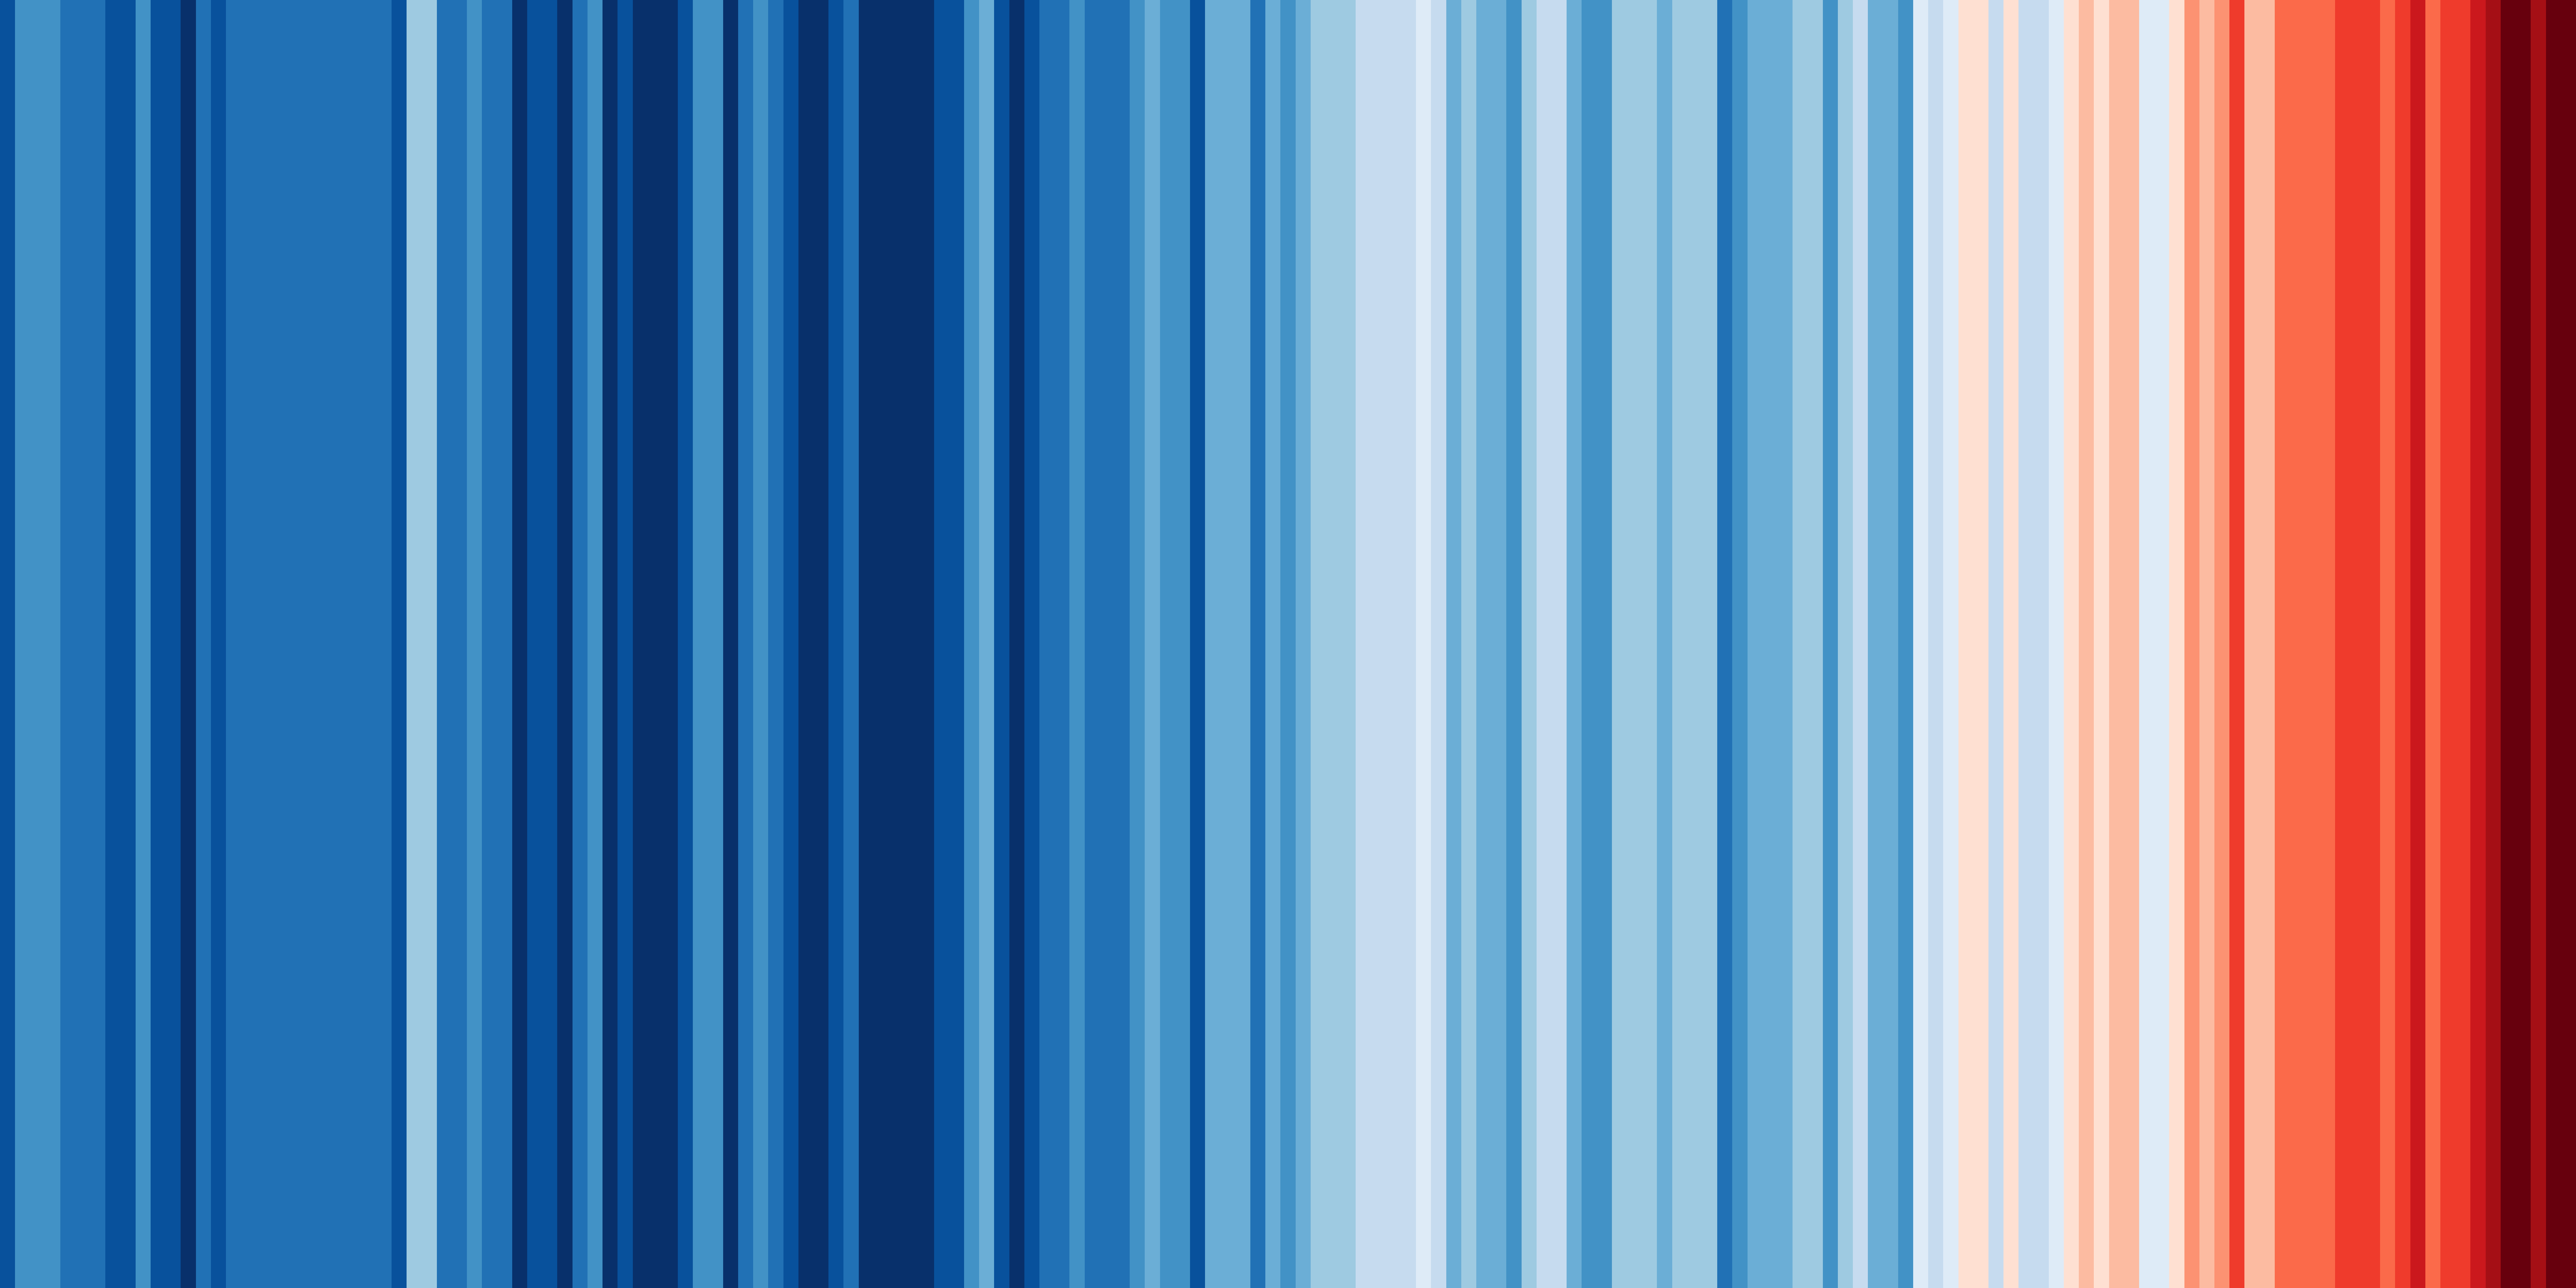
\includegraphics[width=0.6\textwidth]{image_reference/global.png}
    \caption{"Latest global stripes" (1850-2020) by Edward Hawkins}
    \label{fig:global}
\end{figure}

\noindent 
Known as the ``warming stripes," this chart cleverly employs blues to indicate cooler-than-average years and reds to signify hotter-than-average years. Its influence reached far and wide, gracing the front pages of major media outlets and featured in news broadcasts worldwide. It became a symbol in climate change demonstrations. Arguably, it stands as one of the most iconic graphics in modern times.\\

\noindent
\textbf{Misuses of Data Visualisation — Case 1}

\noindent
Having observed the remarkable effectiveness of data visualisations, the significance of employing them correctly becomes apparent. The improper use of data visualisations holds the potential to significantly influence the public in misleading ways, resulting in undesired consequences.\\

\noindent
In fact, inappropriate data visualisation can conceal trends rather than reveal them. Figure~\ref{fig:misuse1} \cite{lie, liestats} illustrates an instance of this issue. On the left-hand side of the figure, an inappropriate scale is used — the y-scale ranges from 0 to 30 million dollars. In this way, the fluctuations in payroll spending are obscured. Conversely, on the right-hand side, a significant increase of over 500,000 dollars in just two months can be observed due to the use of a different scale. This revelation is substantial; considering inflation, 500,000 dollars in 1937 is worth well over 10 million dollars today \cite{worth}.\\

\begin{figure}[H]
    \centering
    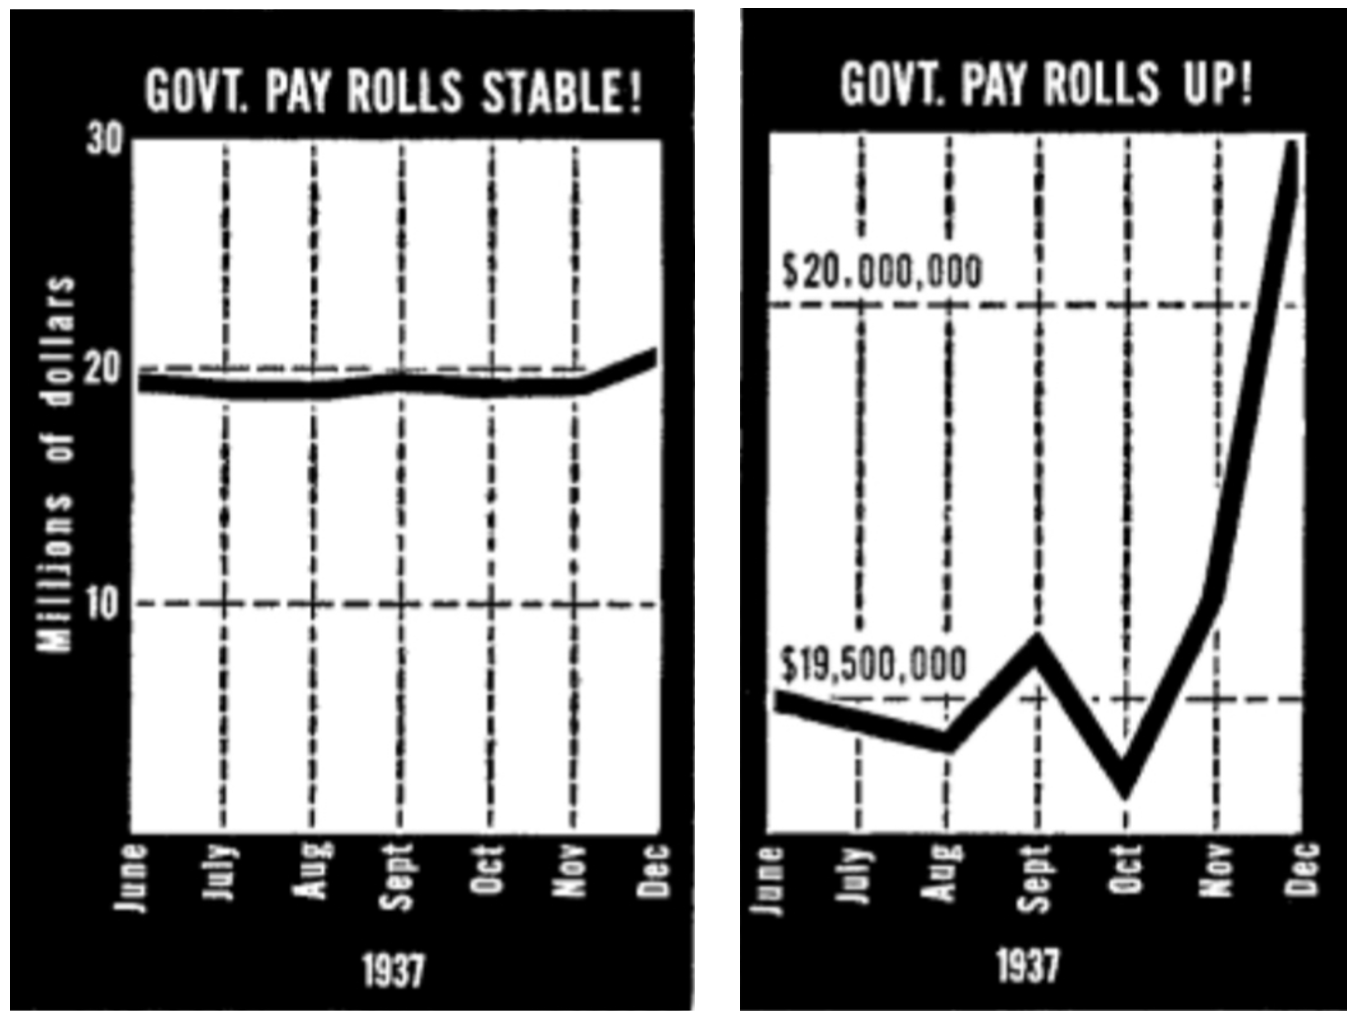
\includegraphics[width=0.6\textwidth]{image_reference/misuse1.png}
    \caption{Incomplete Data Analysis by Miguel de Carvalho, ``How to lie with statistics"}
    \label{fig:misuse1}
\end{figure}

\noindent 
Thus, the scale used in graphs serves as a critical tool, enabling the clear representation of data. However, it also holds the potential to mislead if not employed appropriately. The manipulation of scales can distort the interpretation of data, leading to misrepresentations of reality.\\

\noindent 
\textbf{Misuses of Data Visualisation — Case 2}

\noindent
One striking example of data visualisation misuse is found in the Kallikak Family tree — one of the most prominent eugenic narratives of the 20th century.\\

\noindent
The visualisation shown in Figure~\ref{fig:familytree} \cite{ktree}, was created by the psychologist Henry Goddard and presented in his 1912 book, ``The Kallikak Family: A Study in the Heredity of Feeble-Mindedness." Goddard's narrative centered around Martin Kallikak, a soldier who, in addition to his marriage to a respected citizen, had a one-night stand with a ``feeble-minded" maid. Goddard believed that intellectual disabilities were inherited traits. In Goddard's account, the legitimate family was successful, while the children of the ``feeble-minded" maid were labeled as ``the lowest types of human beings." However, research has since revealed that the entire story was fictitious, as there was no record of the maid's existence \cite{fakedata}.\\

\begin{figure}[H]
    \centering
    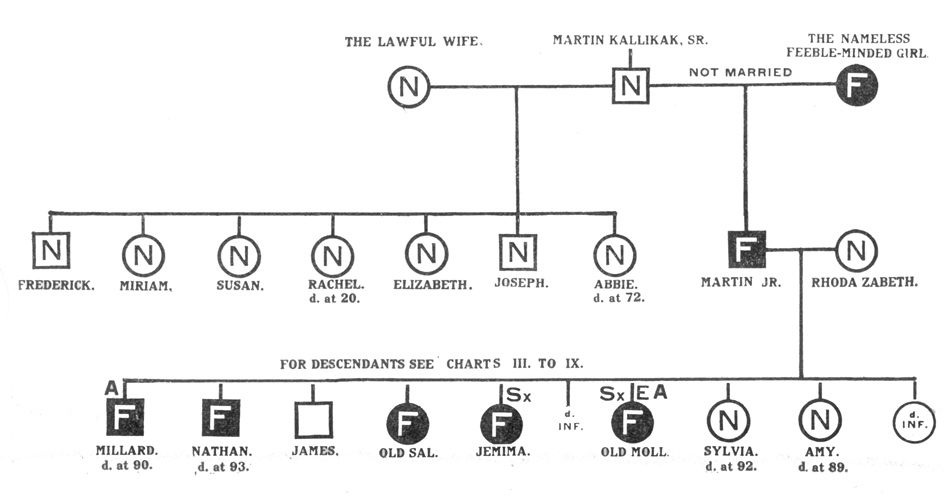
\includegraphics[width=0.7\textwidth]{image_reference/familytree.jpg}
    \caption{The Kallikak Family tree (1912) by Henry Goddard}
    \label{fig:familytree}
\end{figure}

\noindent
Regrettably, the Kallikak family tree became a central element in the eugenics movement. Figure \ref{fig:familytree} was featured in the 1935 Nazi propaganda film ``Das Erbe" (The Inheritance), which was used to promote public acceptance of Nazi eugenics laws. This propaganda laid the groundwork for the forced sterilisation of approximately 400,000 people under Nazi eugenics policies \cite{eugenics}.

\subsection{Computing and Data Visualisation}
\noindent
Over the years, numerous tools have been developed to facilitate the generation of data visualisation. The programme R stands out as a powerful tool for statistical analysis and graphic creation, offering a wide array of functionalities to cater to various data visualisation needs. We will first introduce the commonly used R package \textit{ggplot2}\index{R package!ggplot2}. Then, other key packages used to produce clear and compelling graphs in R will be presented. In this project, R package names such as \textit{ggplot2} are italicised, while R commands like \texttt{faceting} are displayed in a teletype font.\\

\noindent \textbf{The \textit{ggplot2} Package}\\
\noindent
The \textit{ggplot2} package is the main tool in R used to create plots representing datasets of various natures. The foundation of \textit{ggplot2} lies in Leland Wilkinson's \href{https://link.springer.com/chapter/10.1007/978-3-642-21551-3_13}{\textit{The Grammar of Graphics}}, allowing the sequential construction of the individual elements composing a graph \cite{wilkinson2012grammar}. These individual elements are combined to create a unified graphical representation.\\

\noindent
This R package, \textit{ggplot2}, is notable for its robustness and flexibility, enabling the creation of customised graphics rather than adhering strictly to pre-set options. Despite the initial learning curve, \textit{ggplot2} is crafted to be user-friendly, offering sensible defaults and an iterative method for constructing plots. Its focus lies in uncovering the underlying message within the data. Furthermore, \textit{ggplot2} is structured to support layered and annotated graphics that enhance data analysis, especially for beginners and those new to data exploration.\\

\noindent\textbf{Key \textit{ggplot2} Commands}\\
\noindent 
As shown in subsequent sections, it is possible to produce visualisations rather effortlessly by using internal data from R, or even external data, together with \textit{ggplot2}. When using this package, certain key tools are used repeatedly to create visual plots from datasets. Some of these integrals tools for creating sophisticated visualisations are presented subsequently \cite{ggplot2}:\\

\noindent
Firstly, the \texttt{geom} function refers to ``geometric objects". It is pivotal took in \textit{ggplot2} used to specify the type of geometric objects or shapes to be drawn on a plot. Additionally, the \texttt{scales} function enables the adjustment of various mapping details, including colour choices, label formatting, legend arrangement, and more.\\

\noindent Furthermore, the \texttt{coord} function provides the axes and gridlines which aid in structuring and interpreting the graph. Various coordinate systems such as cartesian, polar, and map projections are available. Moreover, \texttt{faceting} is a robust feature enabling the partitioning of a single plot into multiple plots based on factors present in the dataset. This functionality proves particularly beneficial for exploring and presenting data with multiple groups or categories.\\

\noindent The \texttt{theme} function holds significance in customising the non-data elements of plots. The theme system within \textit{ggplot2} allows precise adjustment of aesthetic aspects such as fonts, labels, legends, and background colours. This tool is essential for enhancing plot readability and creating visually captivating graphics tailored to specific audiences or publication requirements.\\

\noindent \textbf{Key Additional Packages}\\

\noindent The R language, on top of the \textit{ggplot2}, has a wide array of packages facilitating diverse functions. Throughout this project, various packages will be used, each enhancing the analysis and presentation of data.\\

\noindent The \textit{tidyverse}\index{R package!tidyverse} is  collection of R packages designed for data science and manipulation. It includes several packages that work seamlessly together, providing a consistent approach to data processing, visualisation, and analysis.\\

\noindent Some of the key packages included in the collection are widely used packages such as \textit{ggplot2} and \textit{dplyr}\index{R package!dplyr}. Particularly, the \textit{dplyr} package plays a pivotal role in data manipulation and transformation. It enables the filtering, sorting, summarising, and transforming of datasets, thereby streamlining data analysis and management.\\

\noindent Moreover, recent research developments in graphical methods, as discussed in the \href{https://www.tandfonline.com/journals/ucgs20}{\textit{Journal of Computational and Graphical Statistics}} such as t-SNE and Q–Q boxplots. The \textit{Rtsne}\index{R package!Rtsne} and \textit{qqboxplot}\index{R package!qqboxplot} packages have allowed us to implement these methods in the report.

\newpage
\subsection{Datasets}
\noindent
This section provides an overview of the different datasets analysed and visualised in the subsequent chapters.\\

\noindent
\href{https://www.rdocumentation.org/packages/datasets/versions/3.6.2/topics/mtcars}{\textbf{mtcars}}: The dataset was extracted from the 1974 Motor Trend US magazine. It includes the fuel consumption and 10 aspects of automobile design for 32 automobiles (1973–74 models). \hfill (built-in R) \\

\noindent
\href{https://www.rdocumentation.org/packages/datasets/versions/3.6.2/topics/iris}{\textbf{iris}}: The dataset was collected by Edgar Anderson. This dataset was famously used by British statistician Ronald Fisher to demonstrate linear discriminant analysis in 1936. It encompasses 5 flower characteristics for 3 types of iris, each with 50 samples. \hfill (built-in R)\\

\noindent 
\href{https://www.gapminder.org/data/documentation/gd001/}{\textbf{gapminder}}: The dataset was provided by the Gapminder Foundation. It encapsulates key demographic statistics like life expectancy, GDP per capita, and population across various countries spanning multiple years, illustrating global development trends.\\

\noindent
\href{https://www.rdocumentation.org/packages/palmerpenguins/versions/0.1.1}{\textbf{palmerpenguins}}: This dataset contains biometric measurements from three distinct penguin species inhabiting the Palmer Archipelago in Antarctica, namely the Adélie, Chinstrap, and Gentoo penguins. \hfill (built-in R)\\

\noindent
\href{https://www.rdocumentation.org/packages/datasets/versions/3.6.2/topics/ToothGrowth}{\textbf{ToothGrowth}}: The dataset measures the tooth growth of 60 guinea pigs. Each animal was either administered with vitamin C or orange juice.  \hfill (built-in R)\\

\noindent
\href{https://firms.modaps.eosdis.nasa.gov/}{\textbf{Fire in Brazil}}: Open-source fire observation data is provided by NASA. The analysis focuses on Brazil (2013-2022). Note that the dataset contains the variable ``confidence", ranging from 0\% to 100\%. The dataset was filtered with a confidence level of $\ge$ 95\%  to ensure an accurate account of fire occurrences \cite{nasa_confidence}.\\

\noindent
\href{https://www.bankofengland.co.uk/boeapps/database/index.asp?first=yes&SectionRequired=I&HideNums=-1&ExtraInfo=true&Travel=NIx}{\textbf{Exchange Rate}}: The exchange rate data from the Bank of England provides daily spot exchange rates against the pound Sterling from 2005 to the present. This report examines the daily spot rates of the Canadian Dollar, Euro, and US Dollar against the pound Sterling.\\

\noindent
\href{https://cloud.r-project.org/web/packages/DATAstudio/DATAstudio.pdf}{\textbf{Metabolic Syndrome Data}}: The oxygen saturation in blood, for a healthy population of 80 women and a diseased population of 35 women. These data were collected through a survey conducted in North-West Spain. The dataset is accessible via DATAstudio, a collection of datasets from research articles by Miguel de Carvalho.\\

\noindent
\href{https://archive.ics.uci.edu/dataset/477/real+estate+valuation+data+set}{\textbf{Taipei Housing}}: The historical real estate valuation from Sindian Dist., New Taipei City, Taiwan,  available at UC Irvine Machine Learning Repository.\\

\noindent
\textbf{covid\_test\_scores}: The synthetic dataset for simulating COVID-19 Diagnostic Test Scores consists outcomes of two different diagnostic tests for COVID-19, referred to as Score\_Test1 and Score\_Test2. The scores are continuous variables that represent the likelihood of a positive diagnosis, with higher scores indicating a higher probability of infection. The dataset includes a Condition column, which indicates the true condition of each simulated individual, with 1 representing a positive COVID-19 case and 0 representing a negative case.

\newpage 

\section{Theoretical Foundations of Data Visualisation}
\noindent This chapter delves into the core principles and concepts that serve as the base of the field of data visualisation. We seek to understand not only the ``how" but also the ``why" behind the creation of visualisations that captivate and inform.

\subsection{Introduction to Data Visualisation Theory}
Creating effective data visualisations requires familiarity with the robust theoretical framework underlying every chart, graph, or plot. These theoretical underpinnings not only form the basis of data visualisation, but also shape the way in which we represent, perceive, understand, and interpret data.\\ 

\noindent \textbf{Guiding Principles for Data Visualisation}\\
The theoretical framework of data visualisation involves guiding principles dictating the visual representation of data. These principles include accuracy, emphasising faithful reflection of underlying data to reduce distortion or misinterpretation; simplicity, advocating for streamlined visuals to convey information effectively; clarity, ensuring visuals are easily understood without unnecessary complexity; relevance, presenting information pertinent to the message or question addressed; and consistency, maintaining uniform use of visual elements like colour coding and labeling throughout a visualisation \cite{grant2018data}.\\

\noindent \textbf{Theoretical Framework and Visual Perception}\\
Furthermore, understanding how the human brain processes visual information is a fundamental aspect of data visualisation theory. This knowledge plays a crucial role in designing visualisations that effectively connect with viewers. It encompasses several key considerations which will be studied subsequently: the Gestalt Principles, concerned with how visual elements are grouped and interpreted; Colour Theory, involving the strategic use of colour contrasts and harmonies to improve clarity; and the management of Cognitive Load, which emphasises the importance of reducing mental effort needed to process information.

\subsection{Data Types and Visualisation Techniques}
Understanding the nature of the data is a key prerequisite before delving into discussions about data representation. Data comes in various types, and selecting the appropriate visualisation technique hinges on recognising these distinctions. In this section, the key data types are categorised and matched with their most suitable visualisation techniques.

\subsubsection{Categorisation of Data Types}
Data can be broadly categorised into four main types \cite{wilkinson2012grammar}: 
\begin{itemise}
    \item \textbf{Nominal data}: represents categories or labels without any inherent order. Examples include colours and gender categories.
    \item \textbf{Ordinal data}: implies a meaningful order or ranking among categories but lacks equal intervals between them. Examples include survey responses (eg. "very satisfied”, “satisfied”, “neutral”, “dissatisfied”, “very dissatisfied”).
    \item \textbf{Interval data}: possesses ordered categories with equal intervals between them, but it lacks a true zero point. An example is temperature, measured in Celsius or Fahrenheit.
    \item \textbf{Ratio data}: includes ordered categories with equal intervals and a meaningful zero point. Examples are age and income.
\end{itemise}
\\

\noindent \textbf{Matching Data Types with Appropriate Visualisation Techniques}\\
\noindent Various data types demand specific visualisation methods for optimal representation. For nominal data, bar charts and stacked bar charts are effective in displaying categorical information and relative proportions. Ordinal data benefits from ordered bar charts, dot plots, or even stacked bar charts, maintaining the ranking and order of categories. Moreover, interval data is best visualised using line charts, histograms, and box plots, showcasing trends and distributions without assuming a true zero point. Finally, ratio data is effectively represented through scatter plots, histograms, and line charts, enabling precise comparisons and measurements due to the presence of a meaningful zero point \cite{healy2018data}. An example of each of these is represented in Figure~\ref{fig:data-plots}, where artificial data from a class of 4th-year university students is visualised.

\begin{knitrout}\scriptsize
\definecolor{shadecolor}{rgb}{0.969, 0.969, 0.969}\color{fgcolor}\begin{figure}[H]

{\centering 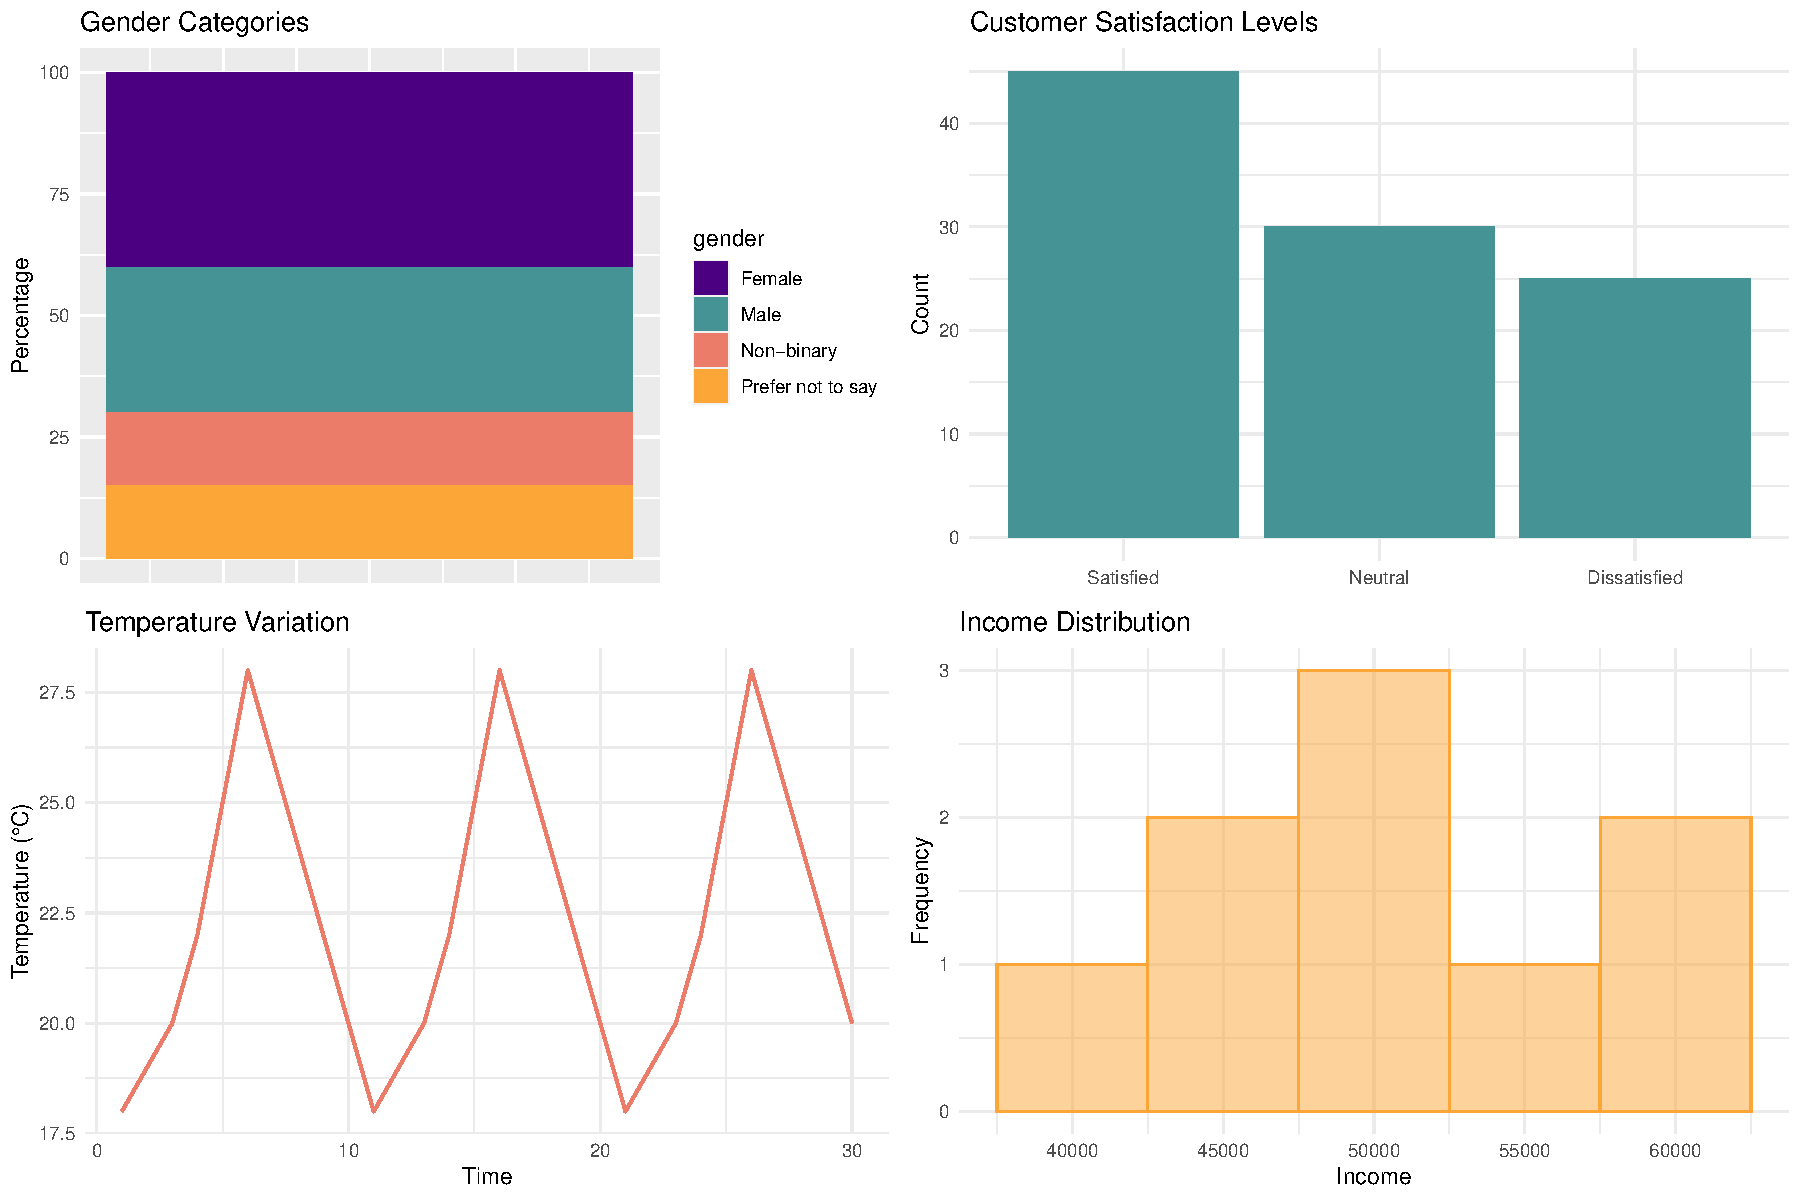
\includegraphics[width=\maxwidth]{figure/beamer-data-plots-1} 

}

\caption[Different types of visualisation techniques according to the data type]{Different types of visualisation techniques according to the data type}\label{fig:data-plots}
\end{figure}

\end{knitrout}

\subsection{Data Abstraction and Representation}
The transformation of complex, raw data into simplified and comprehensible formats by focusing on its essential characteristics and hiding unnecessary details is a pivotal step in data representation \cite{ward2010interactive}. This process, known as data abstraction, involves distilling complex datasets into visual forms that convey insights. In this section, we explore the hierarchies and levels of abstraction in data visualisation, and the critical trade-offs between abstraction and the potential loss of information.

\subsubsection{Hierarchies and Levels of Abstraction}
Hierarchies of abstraction enable the representation data at varying levels of detail: 
\begin{enumerate}
    \item \textbf{Low-Level Abstraction}: At the lowest level, raw data is preserved in its most detailed form. This might include individual data points, measurements, or unprocessed text.
    \item \textbf{Mid-Level Abstraction}: At the mid-level, data is grouped or aggregated to provide a broader overview. For example, hourly data points may be aggregated into daily or weekly averages.
    \item \textbf{High-Level Abstraction}: At the highest level, data is represented in a condensed and abstracted form, often as summary statistics or key insights. Thus, this level provides a "big-picture view" of the data.
\end{enumerate}

\noindent 
These different levels of abstraction are represented in Figure~\ref{fig:abs-plots}, where the mtcars dataset is represented. The first visualisation is a scatter plot that provides detailed information about the relationship between car weight and miles per gallon, with points coloured by the number of cylinders. The second is a bar plot presenting aggregated information about the average miles per gallon for different numbers of cylinders. Finally, the third is an abstract visualisation using a box-and-whisker plot to provide a high-level summary of the distribution of miles per gallon for different numbers of cylinders.

\begin{knitrout}\scriptsize
\definecolor{shadecolor}{rgb}{0.969, 0.969, 0.969}\color{fgcolor}\begin{figure}[H]

{\centering 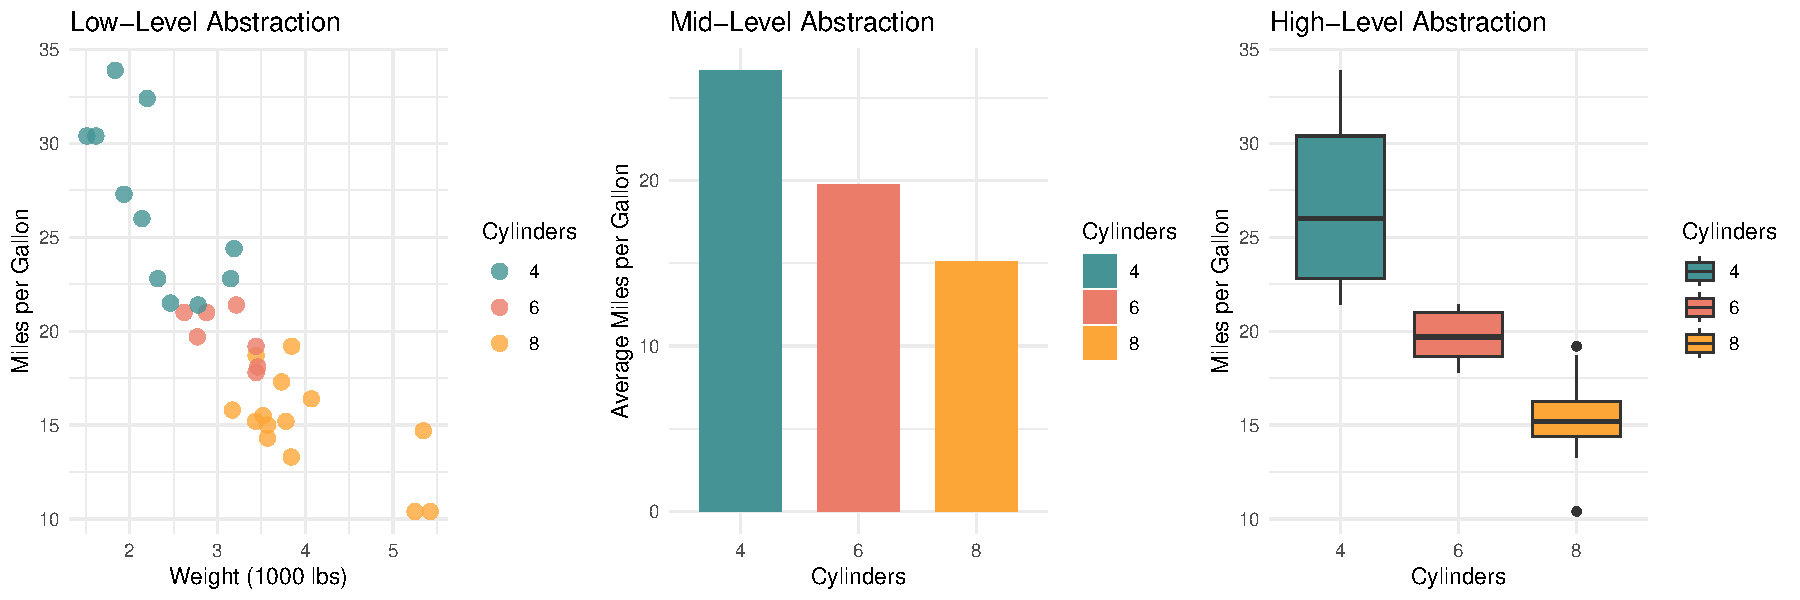
\includegraphics[width=\maxwidth]{figure/beamer-abs-plots-1} 

}

\caption[Mtcars dataset visualised on three different levels of abstraction]{Mtcars dataset visualised on three different levels of abstraction}\label{fig:abs-plots}
\end{figure}

\end{knitrout}
\\
\\
\noindent \textbf{Trade-offs Between Abstraction and Information Loss}\\
While abstraction simplifies complex data, it presents trade-offs. Creators of data visualisations must find a balance between clarity and detail, as well as between generalisation and specificity. Abstraction often increases clarity, but may sacrifice crucial details of the data necessary for certain analytical tasks. It also offers a more generalised view accessible to a wider audience, but may however overlook specific nuances essential for experts.\\ 

\noindent 
In data visualisation, the art of data abstraction lies in finding the right level of detail to effectively convey the intended message while minimising the risk of information loss. This delicate balance is a crucial consideration in the design of informative and meaningful data visualisations.

\subsection{Visual Perception and Cognition}
In this section, human visual perception is explored, along with the application of cognitive psychology principles to data visualisation.\\ 

\noindent \textbf{Human Visual Perception: Decoding Visual Information}\\
Visual perception profoundly influences our understanding of the world. When applied to data visualisation, it shapes the way that individuals engage with and derive meaning from visual data representations.\\

\noindent 
The most significant aspects of human visual perception within the realm of data visualisation include, firstly, pattern recognition, enabling the identification of trends, outliers, and relationships in data representations. Additionally, perceptual grouping, which causes visually similar elements to be grouped together, and thus, influences the interpretation of data clusters and shapes. Moreover, the hierarchy of perception dictates that certain visual attributes are processed more swiftly and effectively than others, such as colour being processed faster than text, influencing the viewer's attention hierarchy \cite{dastani2002role, ward2010interactive}.\\

\noindent \textbf{The Gestalt Principles \index{Gestalt Principles}}\\
Furthermore, the Gestalt Principles play an important role in the realm of visual perception and thus, data visualisation design \cite{rosli2015gestalt}. Key Gestalt principles include proximity, which groups related elements; similarity, that links similar attributes; continuity, aiding trend representation; closure, for implying connections; and symmetry, for balance and aesthetics in visualisations \cite{todorovic2008gestalt}. \\

\noindent Thus, note how by harnessing the principles of human visual perception and applying insights from cognitive psychology, designers of data visualisations can create visualisations that are not only aesthetically pleasing, but which are also cognitively efficient.	

\subsection{Colour Theory in Data Visualisation}
In this section, the significance of colour in data visualisation, the principles of colour perception and encoding, and the importance of avoiding misleading visualisations through thoughtful colour choices are explored.\\

\noindent \textbf{The Importance of Colour in Conveying Information}\\
Colour significantly enhances the impact and comprehension of data visualisations. Some of the multiple purposes that colour serves in data visualisation include emphasising trends, distinguishing data points, and offering contextual information. It is often used to encode categorical data, differentiating between various groups with distinct colours, and to represent quantitative data by using colour intensity or gradients to portray values or magnitude \cite{healy2018data}.\\

\noindent \textbf{Colour Perception and Colour Encoding in Visualisations}\\
Understanding colour perception is crucial in the field of data visualisation. Key principles involve considering colour discrimination\index{Colour theory!colour discrimination}, ensuring accessibility for individuals with colour vision deficiencies. Figure~\ref{fig:colour-plot} illustrates how impactful this is by comparing what is be perceived by "normal" observer, and what is perceived an observed with a colour vision deficiency when a specific colour palette is used. Furthermore, careful selection of colour schemes aligned with the intended message is essential — for instance, using warm colours like red and orange to indicate caution or warmth, and cool colours like blue and green to convey calmness or coldness. Additionally, attention should be paid to how colours interact when combined; certain combinations might create visual vibrations, optical illusions, or impact text legibility.\\

\begin{knitrout}\scriptsize
\definecolor{shadecolor}{rgb}{0.969, 0.969, 0.969}\color{fgcolor}\begin{figure}[H]

{\centering 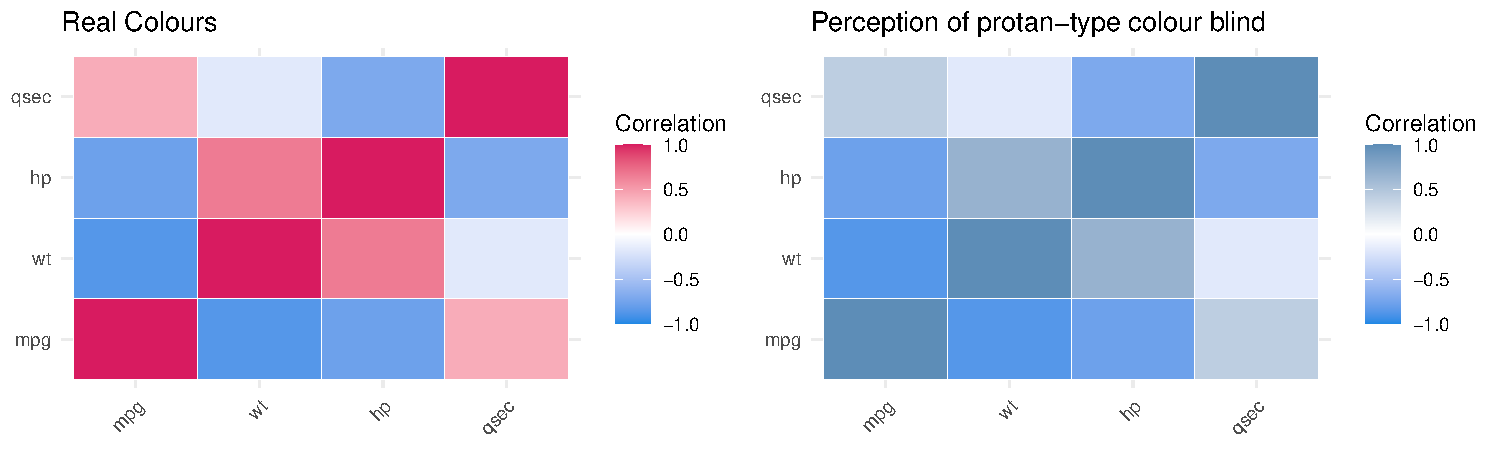
\includegraphics[width=\maxwidth]{figure/beamer-colour-plot-1} 

}

\caption[Colour perception of a heatmap for by a colour-blind person]{Colour perception of a heatmap for by a colour-blind person}\label{fig:colour-plot}
\end{figure}

\end{knitrout}

\noindent \textbf{Avoiding Misleading Visualisations Due to Colour Choices}\\
Misleading visualisations often stem from inappropriate or deceptive use of colour. To avoid this, maintaining consistency in colour usage throughout the visualisation is essential. Furthermore, employing a uniform colour scheme for similar data categories or elements helps establish coherence and understanding. Finally, it's crucial to avoid colour choices that distort or exaggerate the data. Overly intense or contrasting colours might mislead interpretations, emphasising the necessity for judicious colour selection.

\subsection{Cognitive Load and Visual Complexity}
%\setsbsecprefix{Cognitive Load and Visual Complexity}
In data visualisation, achieving a balance between complexity and cognitive load is essential. Cognitive load significantly influences how viewers engage with and comprehend presented data, and finding a balance is crucial to effectively convey information without overwhelming the viewer's cognitive capacity \cite{tufte2001visual}. This section explores the concept of cognitive load in visualisations, strategies to reduce cognitive load while maintaining complexity, and techniques to combat information overload through simplification.

\subsubsection{Strategies to Reduce Cognitive Load While Maintaining Complexity}
Several strategies can be employed to mitigate cognitive load while preserving complexity. Firstly, establishing a clear visual hierarchy using size, colour, and contrast helps direct attention to crucial elements. This strategy is used to simplify the graph on the left side of Figure~\ref{fig:cogload-plot}, to the one on the right side. Secondly, simplifying labels and text by avoiding unnecessary complexity ensures information is clear and easily digestible.\\

\noindent Furthermore, employing interactive features like tooltips\index{Visual complexity!tooltips} and drill-down functionality\index{Visual complexity!drill-down functionality} can assist in providing additional information when required or desired by the observer, while reducing the density of static visualisations.\\

\begin{knitrout}\scriptsize
\definecolor{shadecolor}{rgb}{0.969, 0.969, 0.969}\color{fgcolor}\begin{figure}[H]

{\centering 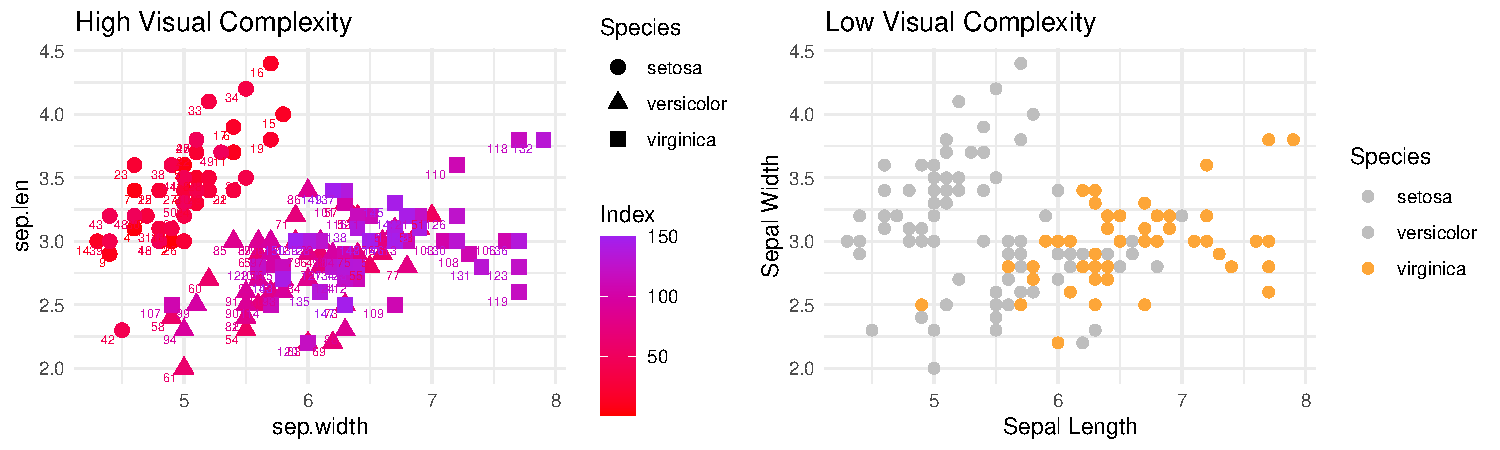
\includegraphics[width=\maxwidth]{figure/beamer-cogload-plot-1} 

}

\caption[High versus low cognitive load demand through the reduction of visual complexity]{High versus low cognitive load demand through the reduction of visual complexity}\label{fig:cogload-plot}
\end{figure}

\end{knitrout}

\subsubsection{Information Overload and Simplification Techniques}
Addressing information overload in visualisations requires the strategic application of simplification techniques. The filtering technique enables focused data selection, while data reduction aggregates information to highlight overarching trends. Furthermore, storyboarding structures data presentation, aiding in contextual comprehension, and prioritisation ensures critical information is prominently displayed, elevating the visualisation's clarity and impact. These strategies collectively combat overwhelming data or excessive visual elements, enhancing comprehension and the effective communication of insights to viewers.

\subsubsection*{Chapter Overview and Further Reading References}

\noindent This chapter delves into the theoretical underpinnings of data visualisation, drawing upon established concepts elucidated in academic literature. Notably, the first chapters in Robert Grant's comprehensive work, \href{https://www.taylorfrancis.com/books/mono/10.1201/9781315201351/data-visualization-robert-grant}{\textit{Data Visualization: Charts, Maps, and Interactive Graphics}} (2018), offers in-depth exploration of these concepts.

\newpage

\section{Univariate Data Visualisation Methods}

\noindent This chapter initiates the discussion regarding data visualisation methods. Particularly, it introduces techniques for graphically representing for datasets of the simplest nature — that is, single-variable datasets. It focuses on histograms, bar charts, the kernel density estimate, time series analysis, and ROC Curves. 

\subsection{Histograms}

\noindent Histograms are essential tools in univariate data visualisation. They provide a concise yet comprehensive overview of the frequency or density distribution of a single variable in a dataset. This chapter explores the construction of two primary types of histograms: classic frequency histograms and density histograms. Additionally, it illustrates their utility through the exploration of a practical application using the iria dataset.

\subsubsection{Classic Frequency Histograms}

\noindent A classic histogram is a visual representation of the distribution of a (numerical) dataset. It is composed by a series of contiguous rectangles, also known as ``bins", each representing a range of data values. The height of each of these corresponds to the frequency or count of data points within that range, depending on the type of histogram. On a cartesian coordinate system, typically, the x-axis shows the endpoints of each bin, and the y-axis represents count or frequency. Hence, histograms facilitate, among other thing, the visualisation of the distribution, spread, and central tendency of datasets.\\

\noindent \textbf{Mathematical Notation}\\
\noindent Suppose the data points within a datset are partitioned into $k$ non-overlapping bins, denoted as $B_1, \dots, B_k$ such that $B_i = [t_i, t_{i+1})$ for $i = 1, \dots, k-1$. Here, $t_i$ and $t_{i+1}$ represent the lower and upper boundaries of the $i$-th bin, respectively.\\

\noindent Then, the classical frequency histogram of the data can be represented as a set of $k$ bars, where the height of the $i$-th bar corresponds to the frequency or count of data points falling within the interval $B_i$.\\

\noindent \textbf{Theory of Bin Number and Bin Width\index{Histograms!bin}}\\
\noindent The classical frequency histogram can be fully described by two main factors: the bin width $b$, and the bin origin $t_{0}$. However, in order for the bin counts to be comparable, the bins should all have the same width. Furthermore, it is essential to correctly choose the number of bins, since these have a huge impact on how the data is displayed and interpreted. Too few bins may hide the information in a dataset, and too many bins can cause a lot of noise in a dataset.\\

\noindent Sturges' Rule\index{Histograms!Sturges' Rule}, established by Herbert Sturges in 1926, offers a systematic approach to determining the optimal number of bins constructing a frequency histogram \cite{scott2015multivariate}. This rule is based on the concept of normality, with the binomial distribution, $B(n,p = 0.5)$, serving as a model for an optimally constructed histogram. It links the binomial distribution with normally distributed data, providing a basis for selecting the number of bins to achieve a histogram resembling a normal density curve.\\

\noindent The rule suggests setting the number of bins, denoted as $k$, to \[ k = 1 + \log_{2} n, \] where $n$ represents the sample size. This formula stems from constructing a frequency histogram with $k$ bins, each of width 1 and centered on the points $i = 0,1,\dots, k - 1$. The bin count of the $i$-th bin is chosen to be the binomial coefficient $\binom{k-1}{i}$. As $k$ increases, this ideal frequency histogram assumes the shape of a normal density with mean $(k - 1)/2$ and variance $(k - 1)/4$. The total sample size is:
\[ n = \sum_{i=0}^{k-1} \binom{k-1}{i} = (1+1)^{k-1} = 2^{k-1}, \]
by the binomial expansion. Hence, Sturges’ rule follows immediately. \cite{scott2015multivariate}.\\

\noindent Note that Sturges’ rule functions as a number-of-bins rule rather than a win  width rule. Assuming all bins are of equal width, to find the win  width, Sturges’ rule is implemented by partitioning the sample range of the data into the recommended number bins \cite{scott2015multivariate}.

\subsubsection{Density Histograms\index{Histograms!density histograms}}

\noindent A frequency histogram differs from a density histogram by its normalisation, which integrates to 1. That is, let $B_k = [t_k,t_{k+1})$ represents the $k$-th bin, as defined previously. If $t_{k+1} - t_k = b$ for all $k$, the histogram has a fixed bin width of $b$. In a frequency histogram, blocks of height $1$ and width $b$ are stacked in the appropriate bins, resulting in an integral equal to $nb$. Conversely, a density histogram uses blocks of height $1/(nb)$ to ensure each block has an area of $1/n$ \cite{scott2015multivariate}. In this way, the height of each bin represents the probability distribution of the data, such that the total area of the histogram equals 1.\\

\noindent \textbf{Theory of Density Histograms}

\noindent Let $v_k$ denote the bin count of the $k$-th bin, representing the number of sample points falling in bin $B_k$. The density histogram is mathematically defined as:
\[ \hat{f}(x) = \frac{v_k}{nb} = \frac{1}{nb} \sum_{i=1}^{n} I_{[t_k,t_{k+1})}(x_i) \quad \text{for } x \in B_k.\]

\noindent With this definition, it is straightforward to verify that $ \hat{f}(x) \geq 0 $ and that $ \int \hat{f}(x) \, dx = 1 $, ensuring that $ \hat{f}(x) $ is a proper density function.\\

\noindent
The density histogram's bin counts ${v_{k}}$ can be considered as binomial random variables, where each bin count $v_{i}$ follows a binomial distribution $B(n,p_{k})$. The probability $p_{k}$ for each bin is the integral of the density function $f(t)$ over the bin interval $B_{k}$:

$$p_{k} = \int_{B_k} f(t) \, dt. $$

\noindent
Consider the Mean Squared Error (MSE) of the estimator $\hat{f}(x)$ for $x \in B_k$. In this case, we have $\text{E}[v_k] = np_k$ and $\text{Var}[v_k] = np_k(1-p_k)$. Consequently, we can derive expressions for the variance and bias of $\hat{f}(x)$ as follows:
$$\text{Var} \hat{f}(x) &= \frac{\text{Var} \ v_{k}}{(nb)^2} = \frac{p_k(1-p_k)}{nb^2},$$
$$\text{Bias} \hat{f}(x) &= \text{E}\hat{f}(x) - f(x) = \frac{1}{nb} \text{E}v_k - f(x) = \frac{p_k}{b} - f(x).$$

\noindent
The Mean Squared Error (MSE) of an estimator $\hat{f}(x)$ can be bounded using Lipschitz continuity and the Mean Value Theorem (MVT). Assuming $f(x)$ is Lipschitz continuous over a bin $B_k$, with a Lipschitz constant $\gamma_k$, the MSE at $x$ can be expressed as the sum of the variance and the square of the bias. This is denoted by the inequality
\begin{equation*}
\operatorname{MSE}\hat{f}(x) \leq \frac{f(\xi_k)}{nb} + \gamma_k^2b^2,
\end{equation*}
where $\xi_k$ is a point in the bin $B_k$, $n$ is the number of observations, and $b$ is the bin width, reflecting the combined effects of variability and estimation error.

\subsubsection{Histograms in Practice}\\

\noindent In R programming, \texttt{geom\_histogram()} in \textit{ggplot2} facilitates the creation of histograms. This function offers flexibility in adjusting the number and width of bins, allowing for precise control over histogram granularity. Additionally, \texttt{geom\_histogram()} supports aesthetic mappings, enabling users to distinguish data subsets using color, fill, or other graphical attributes.\\

\noindent As the sample size increases, the shape of a histogram often begins to resemble that of a normal distribution. This phenomenon is demonstrated in the histogram depicted on the left side of Figure~\ref{fig:iris-plots}. This histogram was generated using the \texttt{geom\_histogram()} function and iris dataset.\\

\begin{figure}[htbp]
  \centering
  \begin{minipage}[b]{0.48\linewidth}
\begin{knitrout}\scriptsize
\definecolor{shadecolor}{rgb}{0.969, 0.969, 0.969}\color{fgcolor}

{\centering 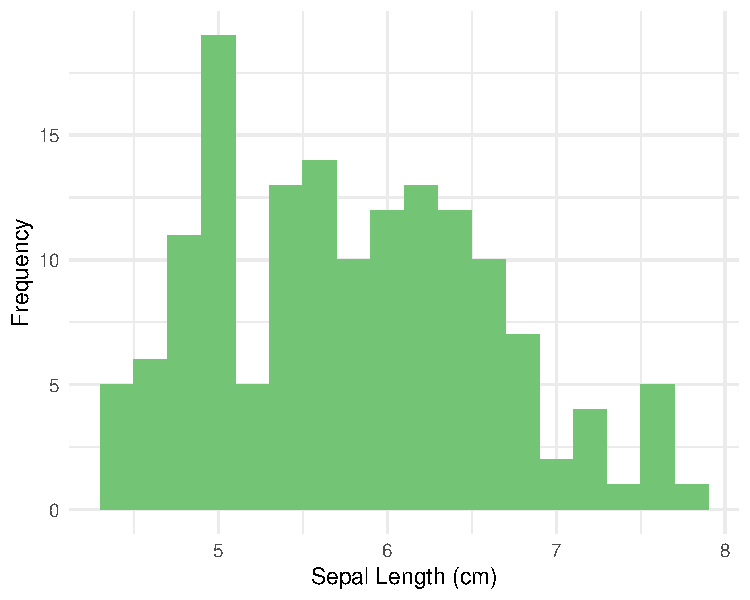
\includegraphics[width=\linewidth]{figure/beamer-hist2-1} 

}


\end{knitrout}
  \end{minipage}
  \hfill
  \begin{minipage}[b]{0.48\linewidth}
\begin{knitrout}\scriptsize
\definecolor{shadecolor}{rgb}{0.969, 0.969, 0.969}\color{fgcolor}

{\centering 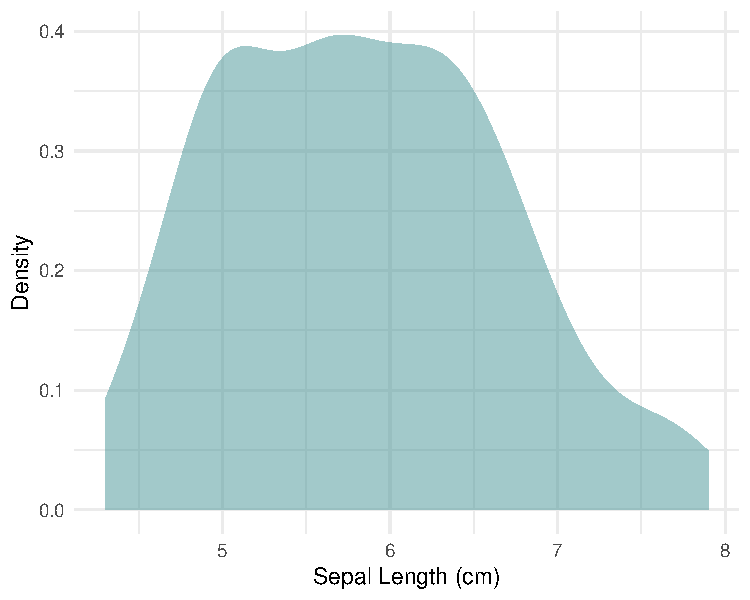
\includegraphics[width=\linewidth]{figure/beamer-kde3-1} 

}


\end{knitrout}
  \end{minipage}
  \caption{Histogram and Kernel Density Estimation of Sepal Length in Iris Dataset}
  \label{fig:iris-plots}
\end{figure}

\noindent The frequency histogram displayed in Figure~\ref{fig:iris-plots} exhibits variable bin lengths, with a constant bin width set to 0.3. The shape of the histogram is slightly shifted to the left, deviating from the symmetric bell shape of a normal distribution. This deviation may indicate some level of asymmetry or non-normality in the data's sepal length variable.

\subsection{Kernel Density Estimation}

Kernel Density Estimation(KDE) evolves from the concept of histogram, offering a method for estimating the the probability density function of a dataset.\\

\noindent 
Kernel Density Estimation (KDE) is an advancement from the traditional histogram method, providing a means to estimate the probability density function of a dataset. It is an extremely valuable tool in statistics, offering a smoother representation compared to discrete histograms by generating a smooth curve from dataset values. KDE is used to infer the distribution of a population based on a limited sample. The outcome of kernel density estimation yields an estimate of the sample's probability density function, allowing for the determination of key characteristics of the data distribution, such as the regions where data is concentrated.\\

\noindent
The KDE algorithm uses a parameter known as bandwidth\index{Kernel density estimation!bandwidth}, which influences the smoothness of the resulting curve. Adjusting the bandwidth alters the shape of the kernel: a lower bandwidth emphasises points very close to the chosen position, resulting in a "squiggly" estimate. Conversely, a higher bandwidth employs a broader kernel, allowing distant points to contribute and yielding a smoother curve.

\subsubsection{Theory of Kernel Density Estimation}\\

\noindent
The kernel density estimator\index{Kernel density estimation!kernel density estimator} can be expressed as follows:
$$\hat{f}(x; h) = \frac{1}{nh} \sum_{i=1}^{n} K\left(\frac{x - X_i}{h}\right).$$

\noindent
In KDE, the variable $x$ represents the point of density estimation. The total number of data points, denoted as $n$, constitutes the sample size, and all these points are used for estimating the dataset's probability density function. The bandwidth $(h)$ is a crucial parameter that controls the smoothness of the estimation, with smaller bandwidths leading to closer fits to data and larger ones smoothing out details. The kernel function $(K)$, such as the Gaussian or triangular kernel, assigns mass around each data point, influencing the density estimate, while $X_i$ represents the individual sample points that collectively contribute to the estimated density function, guided by the kernel function and the bandwidth\cite{wand1994kernel}.\\

\noindent
By introducing the re-scaling notation $K_h(u) = h^{-1}K(\frac{u}{h})$, we can also write the formula for the KDE in a more compact manner:
$$\hat{f}(x; h) = n^{-1} \sum_{i=1}^{n} K_h(x - X_i).$$

\noindent
Here, the kernel function \( K(x) \) \index{Kernel density estimation!kernel function}is a normalised non-negative function that satisfies $\int K(x) dx = 1.$

\noindent
The mean squared error, $\text{MSE}{\hat{f}(x;h)}$, can be used to quantify the difference for a given $x$ between the "true" density function $f(x)$ and its estimator $\hat{f}(x)$, and with some simple transformation, it can be presented as follows:
$$\text{MSE}{\hat{f}(x;h)}=E[(\hat{f}(x)-f(x))^2]=[\text{Bias}\hat{f}(x)]^2+\text{Var}\hat{f}(x).$$

\noindent
We can see that in order to compute $\text{MSE}{\hat{f}(x;h)}$, we will require expression for the mean and variance value of $\hat{f}(x;h)$. This can be derived from the equation of KDE, and by using the convolution notation, we can get the value of the bias. The bias is the difference between a smoothing of $f$ and $f$ itself. Using similar calculations, we can get the variance, and the MSE by combining the variance and bias. So the MSE is expressed as: 
$$\text{MSE}{\hat{f}(x;h)}=n^{-1}\{(K_h^2 \ast f)(x)-(K_h \ast f)^2(x)\}+\{(K_h \ast f)(x)-f(x)\}^2.$$

\noindent
Now, move our attention to the integration of MSE over all $x$, and it gives a global measure of conformity of $\hat{f}(\cdot;h)$ with $f$, called the mean integrated quare error, MISE, and it is one of measures used to estimate the smoothing parameter:
\begin{align*}
\text{MISE}{\hat{f}(\cdot;h)} &= \int \text{MSE}{ \hat{f}(x; h)} \, dx \\
&= n^{-1} \int \{(K_h^2 * f)(x) - (K_h * f)^2(x)\} \, dx + \int \{(K_h * f)(x) - f(x)\} ^2 \, dx.
\end{align*}

\noindent In Figure~\ref{fig:iris-plots}, the kernel density estimation of the iris dataset is represented. In this case, we use the Gaussian kernel by default, which can be expressed as $K(u) = \frac{1}{\sqrt{2\pi}} e^{-\frac{1}{2}u^2}$. The kernel density curve illustrates the distribution of sepal lengths. Peaks in the curve indicate primary concentration trends of sepal length within the data. A unimodal curve indicates a concentration of sepal lengths for most irises in a specific region. Conversely, a bimodal or multimodal curve would suggest the presence of multiple concentration areas.



\subsection{Bar Charts}
\noindent Bar charts are a crucial tool in data presentation, arranging data into vertical or horizontal bars. The varying lengths of these bars directly correspond to the magnitude of the information they represent. Bar charts excel in comparing classified data, especially when values are closely aligned. This stems from the nature of human perception, as our visual acuity for height surpasses that of other visual elements like area or angles.\\

\noindent Bar charts represent a versatile tool in data visualisation. The vertical bar chart, most popular and commonly recognised, exhibits categories along the x-axis and their frequencies or counts along the y-axis. Horizontal bar charts, rotated 90 degrees, prove beneficial for extended category names or numerous categories, displaying categories on the y-axis and frequencies on the x-axis. Multi-set or grouped bar charts facilitate side-by-side comparisons of sub- groups within categories, available in both vertical and horizontal orientations. Stacked bar charts illustrate classes of values subdivided into sub-classes, often differentiated by colour, where each segment's size signifies its frequency or count, and the total bar length reflects the cumulative total.

\subsubsection{Bar Charts in Practice}\\
\noident Figure~\ref{fig:barcharts} represent data for the ToothGrowth dataset. The two bar charts on in the figure illustrate the impact of varying vitamin dosages on tooth growth, further categorised by supplement type. On the x-axis of both graphs, the three distinct levels of vitamin dosage are presented, while the y-axis indicates the average length of tooth for each dosage.\\

\begin{knitrout}\scriptsize
\definecolor{shadecolor}{rgb}{0.969, 0.969, 0.969}\color{fgcolor}\begin{figure}[H]

{\centering 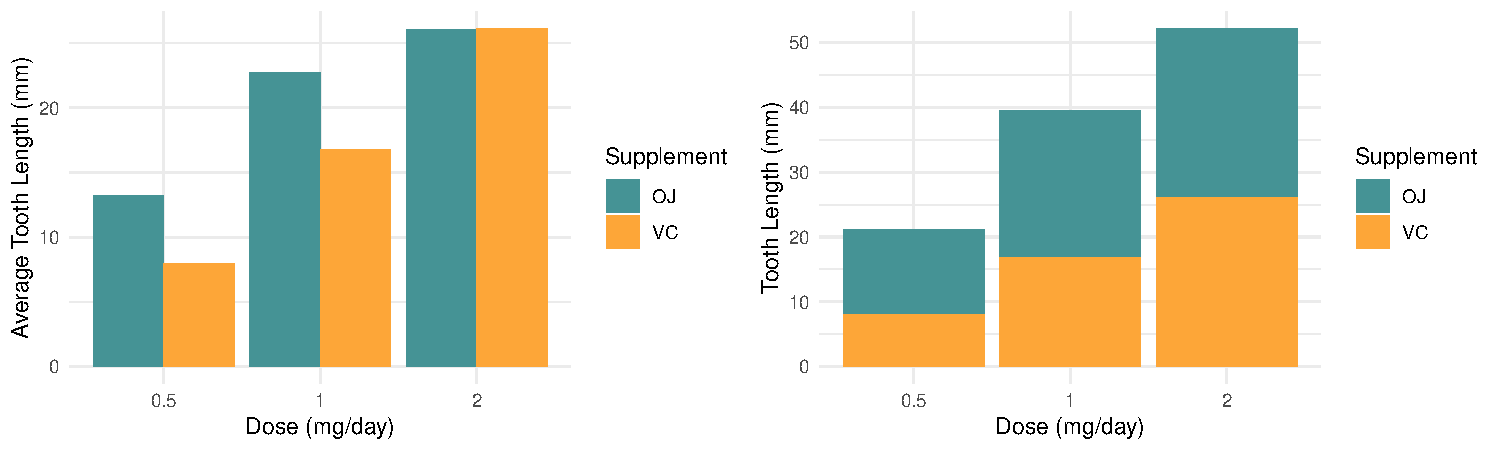
\includegraphics[width=\maxwidth]{figure/beamer-barcharts-1} 

}

\caption[Visualising tooth growth by dosage]{Visualising tooth growth by dosage: A comparison of grouped and stacked bar chart techniques}\label{fig:barcharts}
\end{figure}

\end{knitrout}

\noindent On the grouped bar chart, found on the left of Figure~\ref{fig:barcharts}, due to the side-by-side positioning of the bars, it is easy to note that tooth growth varies not only with the dosage but also with the supplement type. In contrast, the stacked bar graph on the right of Figure~\ref{fig:barcharts} facilitates the understanding of the combined effects of the two supplements at each dosage level. However, compared to the latter, it becomes more challenging to differentiate the individual contribution of each supplement. Thus, highlighting the benefits and downfalls of the different types of bar charts.

\subsection{Line Charts and Time Series}

\noindent
Previous subsections explored histograms, kernel density estimation, and bar charts, which are univariate methods used for analysing independent variables in isolation, revealing patterns and intrinsic properties within data. Now, the focus shifts to univariate methods of dependent variables, specifically line charts, which are crucial for visualising relationships between variables to understanding their interactions and dependencies over time.

\subsubsection{Theory of Line Charts}

Line charts are fundamental tools in data visualisation, particularly useful for displaying time series data. A line chart represents $n$ data points 
$\{(x_i,y_i)\}_{1 \leq i \leq n}$ on a Cartesian coordinate system, with the x-axis often denoting time intervals or ordered categories and the y-axis representing the measured values.\\ 

\noindent
In a line chart, consecutive data points are typically connected by straight lines. The line segment between two points \((x_i,y_i)\) and \((x_{i+1},y_{i+1})\) can be described by the equation of a line in the slope-intercept form: \(y=mx+b\), where \(m\) is the slope and \(b\) is the y-intercept. Also, a series of linear interpolations between pairs of data points could be used. These interpolations assume that the change between two points is uniform or linear. This linear approach is mathematically represented as:
\[
y = y_i + \frac{y_{i+1} - y_i}{x_{i+1} - x_i} \times (x - x_i), \quad  x_i \leq x \leq x_{i+1}.
\]
\noindent
This equation highlights that for any point \(x\) between \(x_i\) and \(x_{i+1}\), the corresponding value of \(y\) on the line chart is determined by a linear relation. This method effectively ``fills the gaps'' between actual observed data points and provides a continuous view of the data.

\subsubsection{Time Series Analysis}

Line charts are well-suited for visualising time series data because they effectively depict changes and trends over time. They provide a clear visualisation of relationships between different time points, making it easy to observe patterns and trends. A time series is a collection of observations $\{x_t\}$, where $t=0,\dots,n$ denotes the time point at which the observation is recorded \cite{Brockwell2016Introduction}. An index set $T_0$ which collects all the time points when observations are available. For instance, $T_0 = \{0,\dots,n\}$ for $n \in \mathbb{N}$. By plotting these data points over time, line charts help in identifying long-term trends, seasonal patterns, and anomalies.\\

\noindent
A time series can be viewed as a realisation of a stochastic process\index{Time series!stochastic process}. A stochastic process $X = (X_t)_{t \in T_0}$ is a collection of random variables $X_t$, where $t$ denotes the time index and $T_0$ the index set. For a fixed event $\omega \in \Omega$ we obtain the realisation of the stochastic process (sometimes also called a sample path) which is given by $x_t = X_t(\omega)$, $t \in T_0$ \cite{Brockwell2016Introduction}.\\

\noindent
A time series $\{X_t\}$ is a moving average process \cite{Brockwell2016Introduction} \index{Time series!moving average process}of order $q$(MA(q)) if it can be expressed as:
\[x_t = \omega_t + \theta_1 \omega_{t-1}+\dots+ \theta_q \omega_{t-q},\]

\noindent
where $\{\omega_t\} \sim \text{N}(0, \sigma^2)$ are independent and identically distributed white noise events and $\theta_1,\dots,\theta_q$ are real valued coefficients.

\subsubsection{Case Example: Visualisation of Exchange Rates}

In Figure~\ref{fig:all exchange rates} daily and 49-day moving average exchange rates of exchange rate data are plotted.\\

\noindent The line graph at the top of Figure~\ref{fig:all exchange rates} presents a comparative visualisation of daily exchange rates for CAD, EUR, and USD against GBP, offering an overview of their trends and relative performance. This plot enables the identification of overall trends and periods of volatility for each currency pair, allowing for an assessment of their stability and strength relative to GBP.\\

\noindent Noticeably, there was a simultaneous and significant decline in all three currencies relative to the GBP. This concurrent decline across diverse currency pairs suggests that the primary driver is a depreciation of the GBP, rather than independent appreciations of the USD, EUR, and CAN. This depreciation of the GBP occurred notably around 2016, coinciding with the onset of the BREXIT process. Typically, financial analysts are most interested in long-term trends. Therefore, filtering out fluctuations and anomalies becomes crucial.\\

\noindent Moreover, a 49-day moving average (MA(49)) was used, as shown in the bottom plot of Figure~\ref{fig:all exchange rates}. This moving average highlights long-term trends while smoothing out short-term fluctuations. This method involves computing the simple average of past observations:
\[\text{MA}_{49}(t) = \frac{1}{49} \sum_{k=t-48}^{t} x_k,\] 
where \( x_k \) denotes the exchange rate on day $k$.\\



\begin{knitrout}\scriptsize
\definecolor{shadecolor}{rgb}{0.969, 0.969, 0.969}\color{fgcolor}\begin{figure}[H]

{\centering 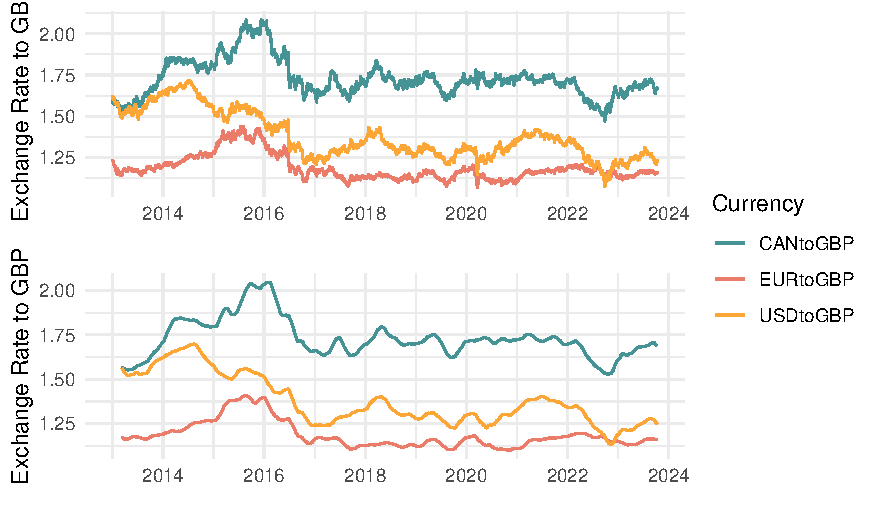
\includegraphics[width=\maxwidth]{figure/beamer-all_exchange_rates-1} 

}

\caption[Daily (top) and 49-day moving average (bottom) exchange rates of CAN, EUR, USD to GBP]{Daily (top) and 49-day moving average (bottom) exchange rates of CAN, EUR, USD to GBP}\label{fig:all exchange rates}
\end{figure}

\end{knitrout}

\noindent
Employing this approach provides a clearer insight into overarching trends in currency movements against the GBP. Overlaying these moving averages onto the daily exchange rates in visualisations offers both a comparative and quantitative perspective.\\

\noindent
\textbf{Autocorrelation Analysis of CNY to GBP Exchange Rate}\\
\noindent
Autocorrelation \index{Time series!autocorrelation}describes the correlation of a time series with its own previous and proceeding values. The autocorrelation function (ACF) measures the linear predictability of the series at lag h, which is the time $t$ with its values at a previous time $t-h$. The mathematical formulation of ACF of time series will be provided in the subsequent paragraph.\\

\noindent
Suppose we have a time series with observations denoted by \( \{x_1, \ldots, x_n \}\). Then the sample mean is given by $\bar{x} = \frac{1} {n} \sum_{t=1}^{n} x_t.$
And the sample autocovariance function \cite{Brockwell2016Introduction} at lag $h$ in days of our time series is
\[\hat{\gamma}(h) := \frac{1}{n} \sum_{t=1}^{n-|h|} (x_{t+|h|} - \bar{x})(x_t - \bar{x}), \quad -n < h < n.\]

\noindent 
Hence, the sample autocorrelation function \cite{Brockwell2016Introduction} at lag $h$ in days is given by

\[\hat{\rho}(h) := \frac{\hat{\gamma}(h)}{\hat{\gamma}(0)} = \frac{\sum_{t=1}^{n-|h|} (x_{t+|h|} - \bar{x})(x_t - \bar{x})}{\sum_{t=1}^{n} (x_t - \bar{x})^{2}}, \quad -n < h < n.\]

\\
\noindent
The value of $\hat{\rho}(h)$ lies between -1 and +1 serves as a measure of correlation. A value close to +1 indicates a strong positive correlation, while a value close to -1 indicates a strong negative correlation. Conversely, a value near 0 suggests little to no linear correlation. In an ACF \index{Time series!ACF}plot, a slow decay indicates a strong relationship between past and present values, while spikes at specific lags may suggest seasonality.\\

\noindent 
In addition, the bounds in an ACF plot help to determine whether the observed autocorrelations are significant or merely due to random fluctuation. The theoretical bounds of the ACF plot are typically set at $\pm 1.96/\sqrt{n}$, where $n$ is the length of the time series. This $\pm 1.96/\sqrt{n}$ formula derives from the assumption of a normal distribution of the autocorrelation coefficient under the null hypothesis of no autocorrelation; And 1.96 corresponds to the 95\% confidence interval of a standard normal distribution. This means that if the ACF of a certain lag falls outside these bounds, the correlation at that lag is statistically significant at the 5\% level, suggesting that the series exhibits autocorrelation at that lag.\\

\noindent
In Figure~\ref{fig:ACF} the ACF for the CNY to GBP exchange rate are visualised to gain a clearer understanding of its time-dependent structure.

\begin{knitrout}\scriptsize
\definecolor{shadecolor}{rgb}{0.969, 0.969, 0.969}\color{fgcolor}\begin{kframe}
\begin{alltt}
\hlcom{# PLOT OF THE AUTOCORRELATION FUNCTION}
\hlstd{acf_data} \hlkwb{<-} \hlkwd{acf}\hlstd{(MyData}\hlopt{$}\hlstd{CNYtoGBP,} \hlkwc{plot} \hlstd{=} \hlnum{FALSE}\hlstd{)}
\hlkwd{plot}\hlstd{(acf_data,} \hlkwc{main} \hlstd{=} \hlstr{""}\hlstd{,} \hlkwc{xlab} \hlstd{=} \hlstr{"Lag h"}\hlstd{,} \hlkwc{ylab} \hlstd{=} \hlstr{"ACF"}\hlstd{)}
\end{alltt}
\end{kframe}\begin{figure}[H]

{\centering 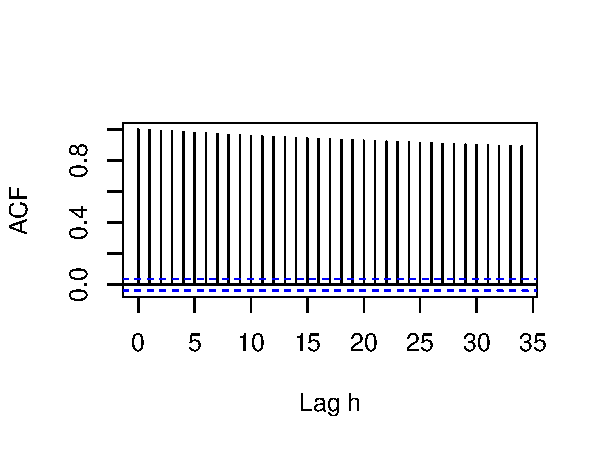
\includegraphics[width=\maxwidth]{figure/beamer-ACF-1} 

}

\caption[Autocorrelation Function at lag h in days of CNY to GBP Exchange Rate]{Autocorrelation Function at lag h in days of CNY to GBP Exchange Rate}\label{fig:ACF}
\end{figure}

\end{knitrout}

\noindent
The ACF plot for the CNY to GBP exchange rate series in Figure~\ref{fig:ACF} reveals that the ACF starts near 1 and decreases gradually. This pattern suggests a strong persistence in the time series, indicating that past values have a significant influence on future values. In time series analysis, such a slow decay in the ACF is indicative of a non-stationary series, where the mean, variance, and autocorrelation structure do not remain constant over time.\\

\noindent 
Also, since the ACF for a wide range of lag falls outside these bounds, the series exhibits strong autocorrelation at those lags. This means that past values of the series have a significant influence on future values.\\

\noindent
This persistent autocorrelation suggests that short-term movements in the CNY to GBP exchange rate are heavily influenced by its recent history. Such a characteristic is crucial for forecasting models, as it implies that recent historical data can be a powerful predictor of near-future trends. Models like ARIMA (Autoregressive Integrated Moving Average), which are well-suited for data with high autocorrelation, may be particularly effective in this context.\\

\noindent
\textbf{Decomposition of Time Series}\\
\noindent
\noindent Time series visualisations offer analysts a clear means of identifying long-term trends and recurring patterns within data. By decomposing the time series, these features become readily apparent. Non-stationary time series data, denoted as $X_t$, can typically be characterized by several distinct components: The trend component $t_t$ illustrates the underlying progression in the series, while the seasonal component $s_t$ describes periodic fluctuations attributed to seasonal factors. Additionally, the residual $r_t$, emphasises irregularities or error component. Consequently, time series decomposition can be encapsulated within two primary models \cite{Brockwell2016Introduction}:\\

\noindent \textbf{Additive Model}: In the additive model, the components are added together:
\[
X_t = t_t + s_t + r_t.
\]
\textbf{Multiplicative Model}: In the multiplicative model, the components are multiplied together:
\[
X_t = t_t \times s_t \times r_t \quad \text{or} \quad \log(X_t) = \log(t_t) + \log(s_t) + \log(r_t).
\]

\noindent In practice, the choice between the additive and multiplicative models often depends on the nature of the time series. If the magnitude of the seasonal fluctuations or the variation around the trend does not vary with the level of the time series, then an additive model is appropriate. If the magnitude of the seasonal fluctuations or the variation around the trend increases or decreases as the time series level changes, then a multiplicative model may be more suitable.\\

\noindent
The R function \href{https://www.rdocumentation.org/packages/stats/versions/3.6.2/topics/decompose}{\texttt{decompose()}} is able to decompose the time series by additive model or multiplicative model. In Figure~\ref{fig:decomposition of time series} a demonstration of such a decomposition is displayed.\\

\noindent
Figure~\ref{fig:decomposition of time series}, displays the decomposition of the the CNY to GBP exchange rate time series into its fundamental components: trend, seasonality, and residual noise by additive model. This decomposition follows the additive model, represented mathematically as $X_t = t_t + s_t + r_t$.\\

\noindent
As illustrated in Figure~\ref{fig:decomposition of time series}, the trend component $t_t$ of CNY to GBP exchange rate exhibits a distinct pattern over time: initially, it shows a gradual decrease and reached crest in 2022, followed by a sudden increase afterwards. It coincides with the tax reduction policy issued by UK government in 2022, which leads to a depreciation of GBP. This trend is pivotal for understanding the broader economic relationship between these currencies. \\

\noindent
Moreover, the seasonal component $s_t$ of the decomposition highlights cyclical fluctuations, indicative of recurrent patterns within the year. These could be attributed to seasonal economic activities, policy changes, or other cyclical factors influencing the currency market. The clear demarcation of these cyclical trends in the seasonal component helps in isolating such effects from the overarching trend.\\



\begin{knitrout}\scriptsize
\definecolor{shadecolor}{rgb}{0.969, 0.969, 0.969}\color{fgcolor}\begin{kframe}
\begin{alltt}
\hlcom{# PLOT OF DECOMPOSITION OF ADDICTIVE TIME SERIES MODEL}
\hlkwd{ggplot}\hlstd{(decomposed_df,} \hlkwd{aes}\hlstd{(}\hlkwc{x} \hlstd{= time,} \hlkwc{y} \hlstd{= value))} \hlopt{+}
  \hlkwd{geom_line}\hlstd{()} \hlopt{+}
  \hlkwd{facet_wrap}\hlstd{(}\hlopt{~}\hlstd{component,} \hlkwc{scales} \hlstd{=} \hlstr{"free_y"}\hlstd{,} \hlkwc{ncol} \hlstd{=} \hlnum{1}\hlstd{)} \hlopt{+}
  \hlkwd{labs}\hlstd{(}\hlkwc{x} \hlstd{=} \hlstr{"Date"}\hlstd{,}\hlkwc{y} \hlstd{=} \hlstr{"Exchange Rate to GBP"}\hlstd{)} \hlopt{+}
  \hlkwd{theme_minimal}\hlstd{()}
\end{alltt}
\end{kframe}\begin{figure}[H]

{\centering 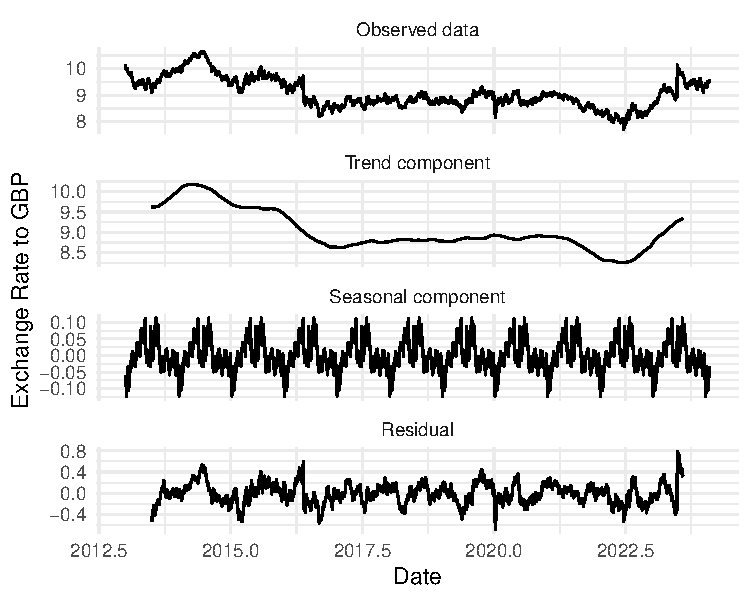
\includegraphics[width=\maxwidth]{figure/beamer-decomposition_of_time_series-1} 

}

\caption[Decomposition of addictive time series model of CNY to GBP exchange rates]{Decomposition of addictive time series model of CNY to GBP exchange rates}\label{fig:decomposition of time series}
\end{figure}

\end{knitrout}

\noindent
Lastly, the residual component $r_t$ encompasses the random, unexplained variations after accounting for the trend and seasonal factors. Analysing these residuals is crucial for understanding the unpredictability in the exchange rate and can be pivotal in risk management and forecasting.

\subsection{ROC Curve}

The Receiver Operating Characteristic (ROC) analysis is a technique used to evaluate the performance of binary classification models at different threshold values. The ROC curve, which plots the true positive rate (TPR) against the false positive rate (FPR), serves as a graphical representation of this evaluation process. Theory and implementation of the ROC curve will be provided below. The ROC curve was first used during World War II for the analysis of radar signals. Following the attack on Pearl Harbor in 1941, the United States military conducted research to enhance the ability to accurately detect Japanese aircraft using radar signals. This research involved measuring the radar receiver operator's proficiency in distinguishing between critical signals, a concept referred to as the Receiver Operating Characteristic (ROC) \cite{rocwiki}.

\subsubsection{Theory of ROC curve}
\noindent
Let's simplify by first consider binary observations. Consider a polulation of size $N$, with diagnosis $\{y_1,\dots,y_N\}$, such that $y = 1$ is positive and $y = 0$ is negative, and the actual diseased condition $\{d_1,\dots,d_N\}$ where $d = 1$ are diseased and $y = 0$ are non-diseased. Given a predictive model, a True positive (TP) is a diseased individual $d_n = 1$ correctly identified as positive $y_n =1$. A False positive (FP) is a non-diseased individual $d_n = 0$ incorrectly identified as positive $y_n =1$. The concept of True negative (TN) and False nagative (FN) are similar. Then, the total number of TP, FP, TN and FN given a predictive model can be expressed as:

\[\text{TP} = \sum^{N}_{n=1} \mathbb{I}(d_n = 1) \mathbb{I}(y_n = 1), \quad \text{FP} = \sum^{N}_{n=1} \mathbb{I}(d_n = 0) \mathbb{I}(y_n = 1),\]

\[\text{FN} = \sum^{N}_{n=1} \mathbb{I}(d_n = 1) \mathbb{I}(y_n = 0), \quad \text{TN} = \sum^{N}_{n=1} \mathbb{I}(d_n = 0) \mathbb{I}(y_n = 0),\]

\noindent
where $\mathbb{I}$ is the indicator function.\\

\noindent
Then, TPR and FPR can be defined as follows:

\[\text{TPR} = \frac{TP}{TP+FN}, \quad \text{FPR} = \frac{FP}{FP+TN}.\]
\\
\noindent
Now let's consider the cases where diagonisis $\{y_1,\dots,y_N\}$ are continuous.\\

\noindent
Suppose we have a threshold c (variable), which we use as the classification criterion defined as follows: \\

\noindent
classify as a positive case $y_n = 1$ if observation $y_n \geq c$,\\
\noindent
classify as a negative case $y_n = 0$ if observation $y_n < c$.\\

\noindent
Then, the True Positive Rate (TPR) and the False Positive Rate (FPR) in the continuous case can be defined as follows \cite{Pepe2003}:


\[\text{TPR}(c) = \mathbb{P}[\hat{y}_n \geq c | d_n = 1], \quad \text{FPR}(c) = \mathbb{P}[\hat{y}_n \geq c | d_n = 0].\]

\noindent
The ROC curve is then the set of points $(\text{FPR}(c), \text{TPR}(c))$ for all possible values of threshold $c$. This curve plots the trade-off between sensitivity (or TPR) and specificity (1 - FPR) across different thresholds. Let $t=\text{FPR}(c)$, then $c = \text{FPR}^{-1}(t)$ and $\text{TPR}(c)= \text{TPR}(\text{FPR}^{-1}(t))$. Hence, let $\text{ROC}(t)= \text{TPR}(\text{FPR}^{-1}(t))$, the ROC curve can be represented as a parametric function of $t$ (classification threshold corresponding to $t=\text{FPR}(c)$), with $t$ varying from 0 to 1:

\[ \text{ROC} = \{ (t, \text{ROC}(t)) \,|\, t \in [0, 1] \}.\]

\noindent
The Area Under the Curve (AUC) provides a single measure of model performance. This definition represents the integral of $\text{ROC}(t)$ over the interval from 0 to 1. It can be defined as:

\[ \text{AUC} = \int_{0}^{1} \text{ROC}(t) dt.\]

\noindent
The larger the AUC\index{Receiver operating characteristic!AUC}, the better the classifier.

\subsubsection{ROC analysis in COVID-19 test}

The COVID-19 pandemic underscores the need for accurate diagnostic tests to differentiate between positive and negative cases \cite{Garcia2021ROCAlly}. An effective mean for evaluating accuracy of various diagnostic tests is the ROC analysis.\\

\noindent
An ideal test minimises FPR, avoiding unnecessary treatments or quarantine. The ROC curve visualises the trade-off between TPR and FPR at various thresholds. A curve arching towards the upper left indicates high sensitivity and low FPR — the hallmarks of a reliable test.\\

\noindent
The Figure~\ref{fig:roc} plots the ROC curve of simulated COVID-19 test data. 



\begin{knitrout}\scriptsize
\definecolor{shadecolor}{rgb}{0.969, 0.969, 0.969}\color{fgcolor}\begin{figure}[H]

{\centering 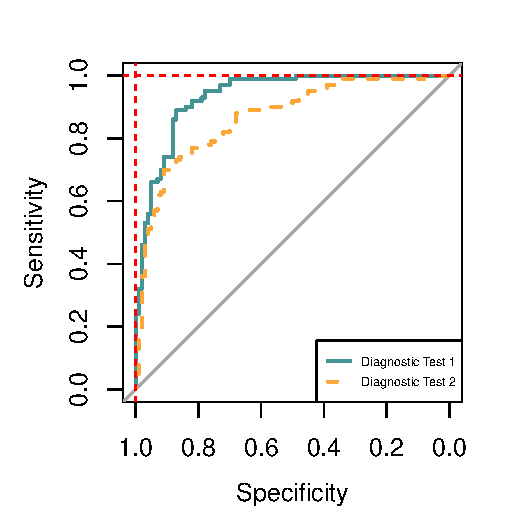
\includegraphics[width=\maxwidth]{figure/beamer-roc-1} 

}

\caption[ROC Curves for Two Diagnostic Tests]{ROC Curves for Two Diagnostic Tests}\label{fig:roc}
\end{figure}

\end{knitrout}

\noindent
From the plot~\ref{fig:roc}, the Diagnostic Test 1 has higher AUC, which is closer to the top left corner. This test is likely to be more accurate in diagnosing COVID-19. It suggests that the test has a higher combined sensitivity and specificity, meaning it can identify positive cases more correctly and has fewer false alarms. Also, the Diagnostic Test 2 has a lower AUC than Test 1, This test is less accurate but still better than random guessing. It may miss more true cases (lower sensitivity) or incorrectly identify healthy individuals as having COVID-19 (higher false positive rate).

\subsubsection*{Chapter Overview and Further Reading References}

\noindent In this chapter, we have delved into the theory behind histograms, density estimators, line charts, time series, and the ROC curve. These concepts are well-established in statistical literature. For further insights into histograms and kernel smoothing, David W. Scott's book \href{https://ebookcentral.proquest.com/lib/ed/detail.action?docID=1895499&pq-origsite=primo}{\textit{Multivariate Density Estimation: Theory and Practice, and Visualization}} (1992) provides comprehensive details of the theory behind these concepts. Additionally, \href{https://link-springer-com.eux.idm.oclc.org/book/10.1007/978-3-319-29854-2}{\textit{Introduction to Time Series and Forecasting}} (2016) by Peter J. Brockwell and Richard A. Davis offers in-depth exploration of line charts and time series theory. Lastly, Margaret Sullivan Pepe's \href{https://ebookcentral.proquest.com/lib/ed/detail.action?docID=1573145}{\textit{The Statistical Evaluation of Medical Tests for Clarification and Prediction}} (2003), particularly Chapters 4 and 5, provides thorough coverage of the ROC curve theory. 

\newpage

\section{Bivariate Data Visualisation Methods}

\noindent This chapter transitions from the study of univariate data visualisations to the exploration of bivariate data. Fundamental bivariate data visualisation methods, including heatmaps, scatter plots, and bubble charts, are introduced, studied, and modeled throughout the chapter. In order to facilitate a more profound analysis of bivariate data, the chapter further delves into the examination of linear regression, as well as LOESS regression. Furthermore, within the context of scatter plots, an intriguing deviation is observed with the incorporation of animated data visualisations.

\subsection{Heatmaps}
The heatmap is a data visualisation technique that uses colour coding to represent different intensities. It can be represented as an $m \times n$ matrix $\mathbf{M}$, with $m$ observations for variable 1 and $n$ observations for variable 2:

$$\mathbf{M} =
\left[
\begin{array}{cccc}
    \mathrm{M}_{11} & \mathrm{M}_{12} & \ldots & \mathrm{M}_{1n} \\  
    \mathrm{M}_{21} & \mathrm{M}_{22} & \ldots & \mathrm{M}_{2n} \\  
    \vdots & \vdots & \ddots & \vdots \\  
    \mathrm{M}_{m1} & \mathrm{M}_{m2} & \ldots & \mathrm{M}_{mn}
\end{array}
\right],
$$

\noindent
where each entry $\mathrm{M}_{mn}$ represent an observation.\\

\noindent Heatmaps aid to convey patterns, trends, and distributions within datasets by visually highlighting areas of high or low density. This facilitates the identification of clusters, outliers, and correlations, aiding decision-making processes across various domains such as finance, biology, and urban planning. 

\subsubsection{Heatmaps in Practice}
\noindent
In this illustrative example, heatmaps of different natures are used to visualise and study fire occurrences in Brazil. The heatmaps depicted in Figure~\ref{fig:fire22} offer a geographically coherent representation of fire occurrences across the country, highlighting regions at high risk. Complementing this spatial representation, the heatmap depicted in Figure~\ref{fig:fire-by-months-fy13-22} elucidates the presence of discernible seasonal patterns in fire occurrences.\\









\begin{figure}[htbp]
  \centering
  \begin{minipage}[b]{0.48\linewidth}
\begin{knitrout}\scriptsize
\definecolor{shadecolor}{rgb}{0.969, 0.969, 0.969}\color{fgcolor}

{\centering 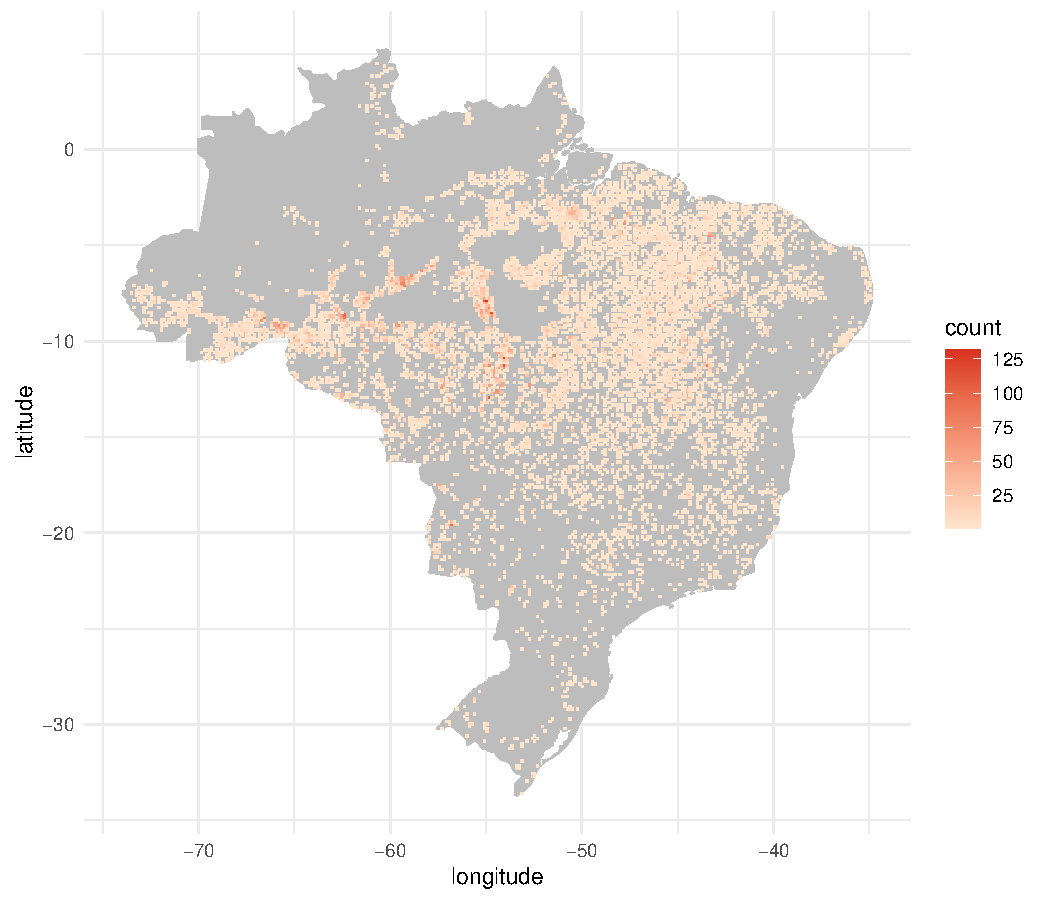
\includegraphics[width=\maxwidth]{figure/beamer-spacetime-fy22-1} 

}


\end{knitrout}
  \end{minipage}
  \hfill
  \begin{minipage}[b]{0.48\linewidth}
\begin{figure}[H]
    \centering
    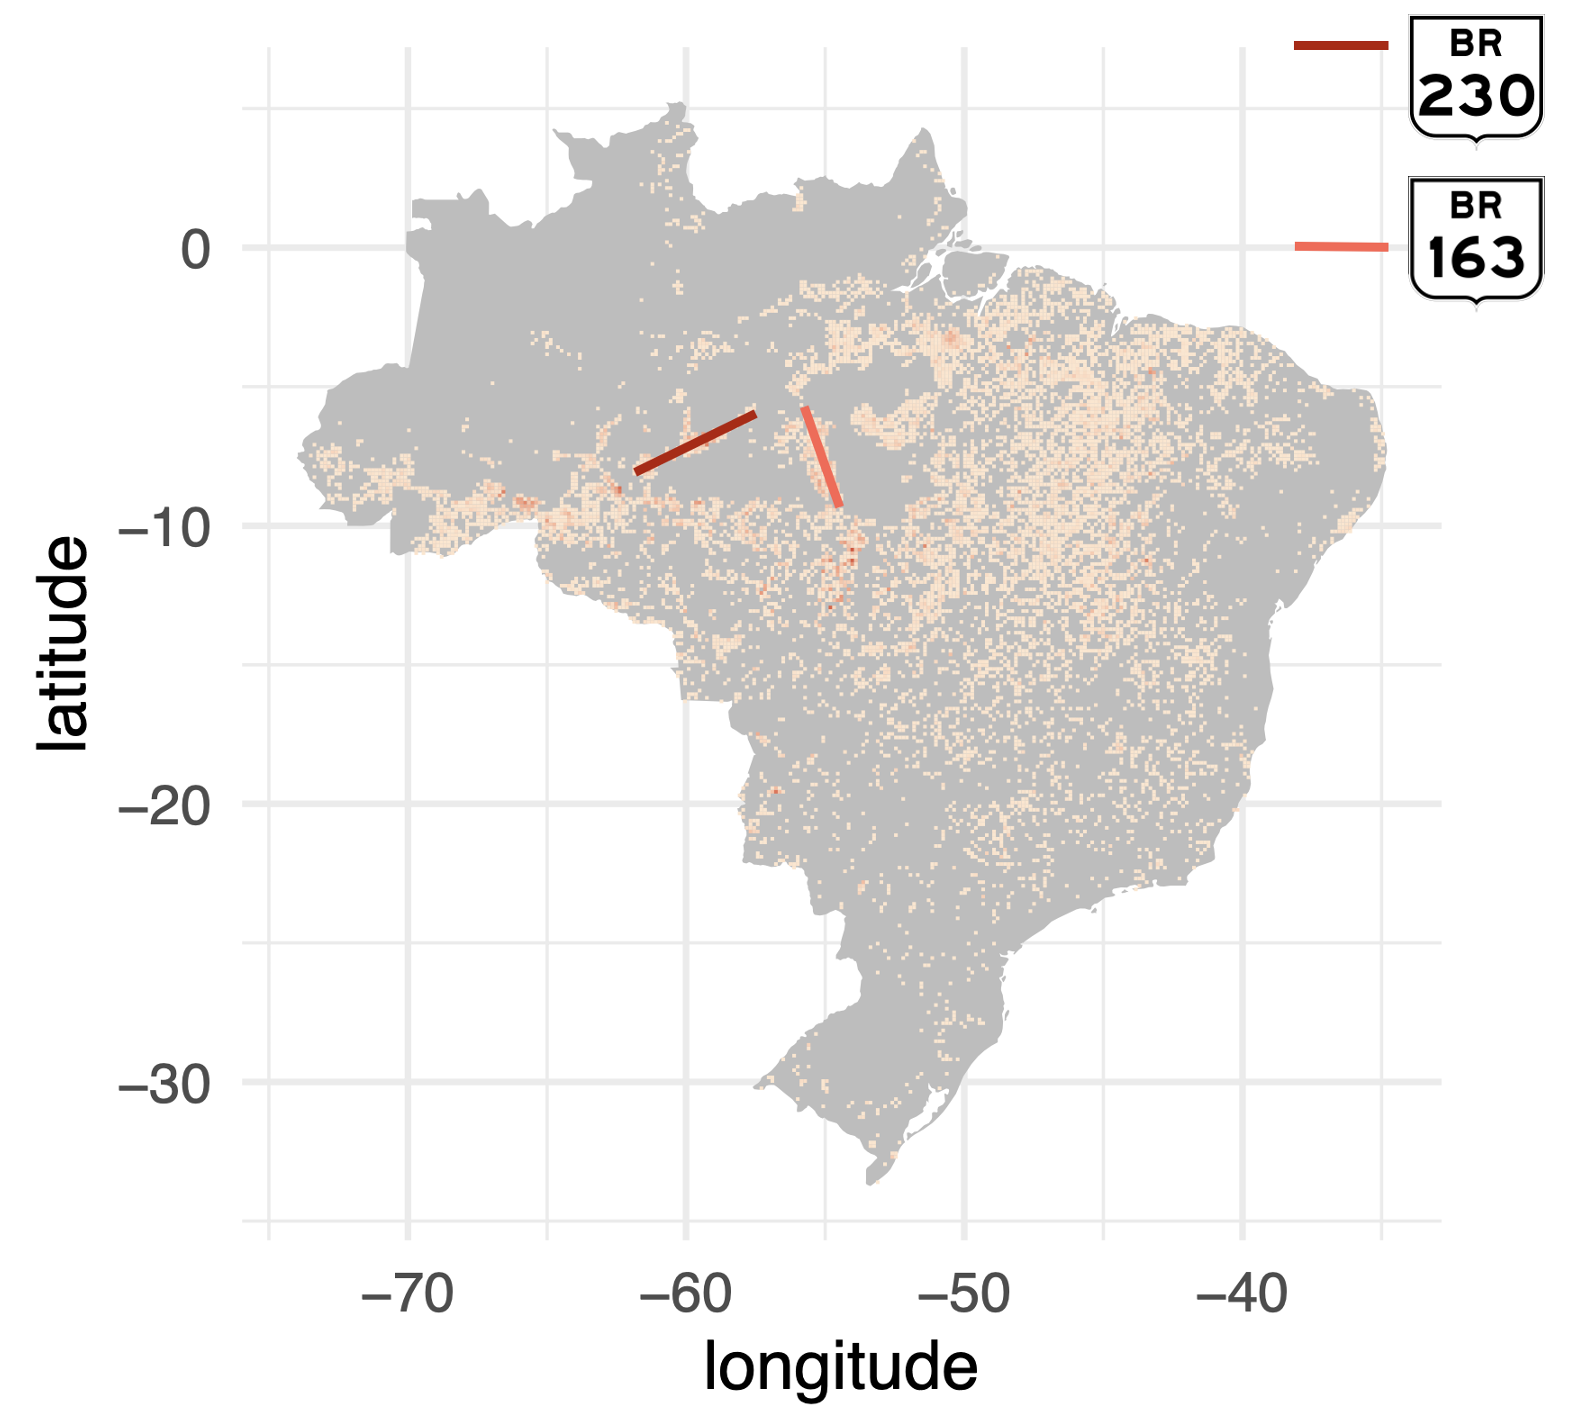
\includegraphics[width=1\linewidth]{image_reference/mapshoot.png}
\end{figure}
  \end{minipage}
  \caption{Geographical fire frequency in Brazil (2022) highlighting unusual high frequency strips}
  \label{fig:fire22}
\end{figure}



\begin{knitrout}\scriptsize
\definecolor{shadecolor}{rgb}{0.969, 0.969, 0.969}\color{fgcolor}\begin{kframe}
\begin{alltt}
\hlcom{# HEATMAP PLOT}
\hlstd{heatmap_plot} \hlkwb{<-} \hlkwd{ggplot}\hlstd{(pivot_table,}
                       \hlkwd{aes}\hlstd{(}\hlkwc{x} \hlstd{=} \hlkwd{factor}\hlstd{(abb_month,} \hlkwc{levels} \hlstd{= custom_order),}
                           \hlkwc{y} \hlstd{=} \hlkwd{as.character}\hlstd{(year),} \hlkwc{fill} \hlstd{= count))} \hlopt{+}
  \hlkwd{geom_tile}\hlstd{()} \hlopt{+}
  \hlkwd{scale_fill_gradient}\hlstd{(}\hlkwc{low} \hlstd{=} \hlstr{"#fff7ec"}\hlstd{,} \hlkwc{high} \hlstd{=} \hlstr{"#d7301f"}\hlstd{)} \hlopt{+}
  \hlkwd{labs}\hlstd{(}\hlkwc{x} \hlstd{=} \hlstr{" "}\hlstd{,} \hlkwc{y} \hlstd{=} \hlstr{" "}\hlstd{)} \hlopt{+}
  \hlkwd{theme_minimal}\hlstd{()} \hlopt{+}
  \hlkwd{theme}\hlstd{(}\hlkwc{axis.text} \hlstd{=} \hlkwd{element_text}\hlstd{(}\hlkwc{size} \hlstd{=} \hlnum{9}\hlstd{))}

\hlkwd{print}\hlstd{(heatmap_plot)}
\end{alltt}
\end{kframe}\begin{figure}[H]

{\centering 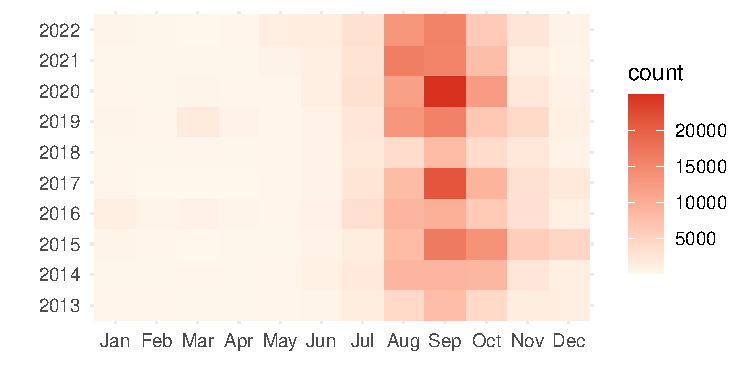
\includegraphics[width=\maxwidth]{figure/beamer-fire-by-months-fy13-22-1} 

}

\caption[Frequency of fire in Brazil (2013-2022)]{Frequency of fire in Brazil (2013-2022)}\label{fig:fire-by-months-fy13-22}
\end{figure}

\end{knitrout}

\noindent
In Figure~\ref{fig:fire22}, it is evident that certain locations exhibit significantly higher fire counts than others. Notably, two distinct strips display unusually high frequencies of fires. The vertical trend aligns with the route of BR-230 (Trans-Amazonian Highway) passing through the city of Apuí, State of Amazonas. Similarly, the horizontal trend corresponds to BR-163 (Brazil Highway) traversing Três Pinheiros in Novo Progresso, State of Pará. Moreover, the western coastal area, characterised by frequent fire occurrences, is proximate to the cities of Vista Alegre do Abunã and Rio Branco. Research indicates that 95\% of active fires, particularly the most intense ones (FRP $<$ 500 megawatts), manifest at the forest edges \cite{forest}. Thus explaining why there would be an intensification of fire occurances in these areas.\\ 

\noindent
Additionally, the seasonal variation in fire frequency is represented in Figure~\ref{fig:fire-by-months-fy13-22}. Notably, an increase in fire occurrences is observed during the months of August to October compared to other periods throughout the year. This temporal pattern aligns with climatological factors such as the onset of the dry season, which escalate the likelihood of fire incidents during these months.\\

\noindent 
These heatmaps can offer policymakers valuable insights for crafting effective preventive measures and firefighting strategies, thus highlighting the powerful and effective nature of this visualisations.

\subsection{Scatter Plots}

A scatter plot is a graphical representation of a set of data points in a two-dimensional coordinate system. Each data point is represented by a dot, and the position of the dot is determined by the values of two variables in the system. Some examples of this type of visualisation can be found in Figures~\ref{fig:abs-plots}, ~\ref{fig:cogload-plot}, and ~\ref{fig:bubble-plot-construction}.\\

\noindent
Generally, in scatter plots the \(Y\)-axis denotes the response, or dependent variable and the \(X\)-axis denotes the explanatory, or independent variable. Each observation of a dataset is mapped to a dot in the 2-dimentional space. Let \((x_i, y_i)\) represent the coordinates of the \(i\)-th data point on the scatter plot produced by mapping a set of data. The scatter plot can be mathematically described as a set of points: \( \{(x_1, y_1), \ldots, (x_n, y_n)\}\) where \(n\) is the number of observations in the set.

\subsubsection{Scatter Plots in Practice}

\noindent The \textit{ggplot2} package in R offers a versatile built-in function for generating scatter plots called \texttt{geom\_point()}. This function works by mapping variables in a dataset to aesthetic attributes of points in a scatter plot, such as position (x and y coordinates), size, color, shape, and transparency.\\

\noindent Illustrations of plots generated in this manner are depicted in Figure~\ref{fig:bubble-plot-construction}. The scatter plots in this figure visually depict relationships between variables in the mtcars dataset.\\

\begin{knitrout}\scriptsize
\definecolor{shadecolor}{rgb}{0.969, 0.969, 0.969}\color{fgcolor}\begin{figure}[H]

{\centering 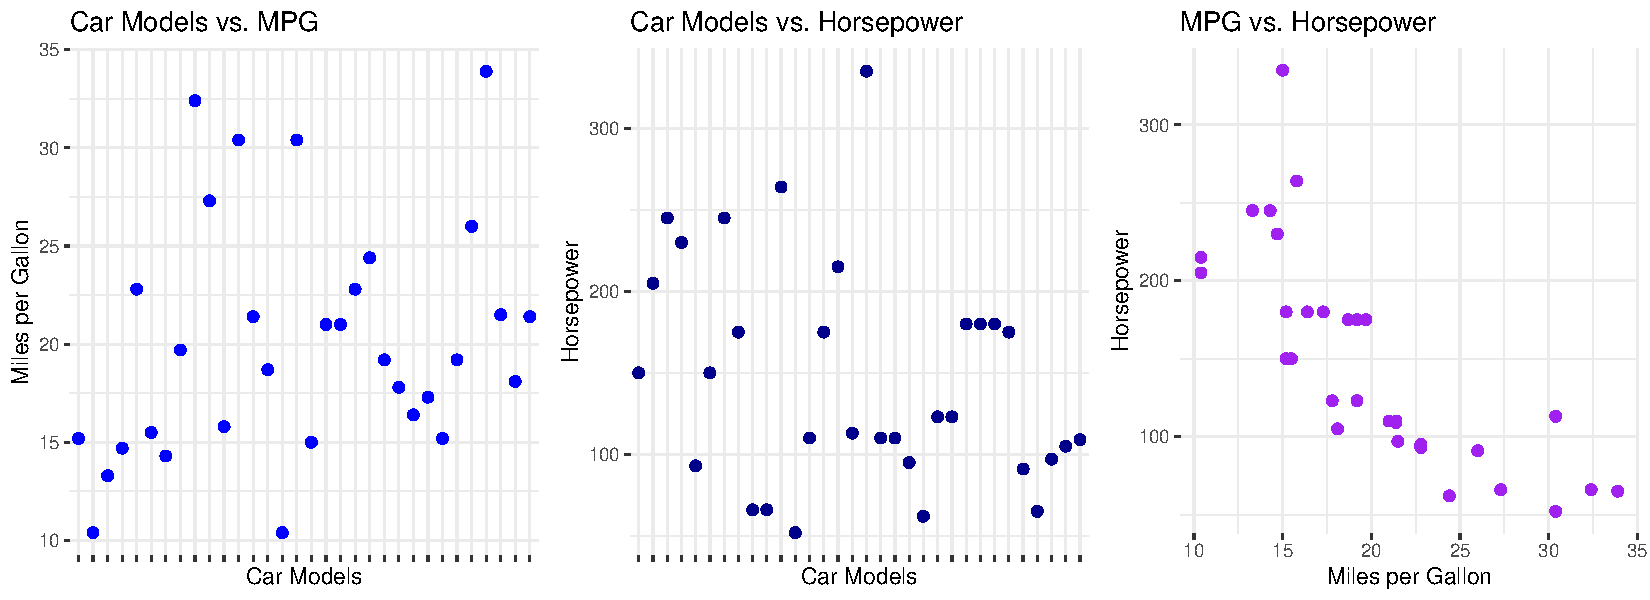
\includegraphics[width=\maxwidth]{figure/beamer-bubble-plot-construction-1} 

}

\caption[Partial scatter plot deconstruction of the mtcars dataset]{Partial scatter plot deconstruction of the mtcars dataset}\label{fig:bubble-plot-construction}
\end{figure}

\end{knitrout}

\noindent The first plot in Figure~\ref{fig:bubble-plot-construction} illustrates the relationship between car models and miles per gallon (MPG), showing potential differences in fuel efficiency among different models. Similarly, the second plot explores the association between car models and horsepower. Finally, the third plot examines the correlation between MPG and horsepower. \\

\noindent As expected, discerning a pattern or clear relationship between variables proves challenging in the first and second scatter plots. This challenge arises from the fact that the variable depicted along the $X$-axis in these plots is the car model, which lacks any relevant ordering that would relate on the technical details of the cars. Conversely, in the third scatter plot, a negative correlation between horsepower and miles per gallon is evident. This relation highlights potential trade-offs between fuel efficiency and engine performance. 

\subsubsection{Animated Scatter Plots}
\noindent While static scatter plots are effective in depicting relationships between two variables, animated scatter plot visualisations take this a step further by introducing, for example, a temporal dimension to the data visualisation. Unlike static plots, animated scatter plots enable the depiction of changes in relationships, clusters, or outliers over time. In R, the $gganimate$ package, building on the foundation of $ggplot2$ package, facilitates the creation of animated plots, including animated scatter plots. 

\subsubsection{\textit{gganimate} in Practice}

\noindent Figure~\ref{fig:gapminder_static} represents the gapminder dataset in a static scatter plot demonstrating the relationship between gross domestic product (GDP) per capita and life expectancy across various countries. GDP per capita is depicted on a logarithmic scale along the $X$-axis to accommodate a wide range of values, while life expectancy is represented on the $Y$-axis. Moreover, the colour each of the dots indicate the country they represent data of.\\

\begin{knitrout}\scriptsize
\definecolor{shadecolor}{rgb}{0.969, 0.969, 0.969}\color{fgcolor}\begin{figure}[H]

{\centering 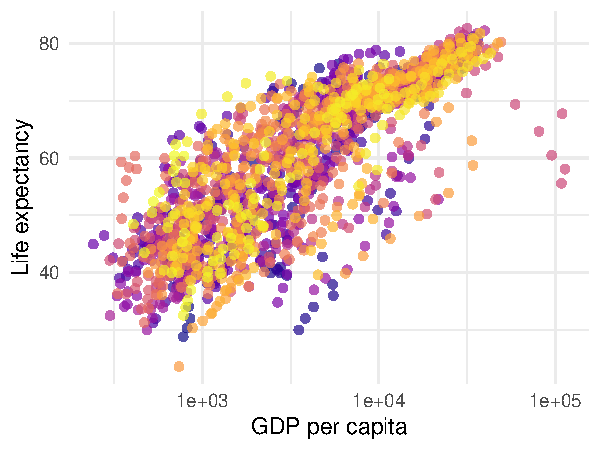
\includegraphics[width=\maxwidth]{figure/beamer-gapminder_static-1} 

}

\caption[Static scatter plot deconstruction of the gapminder dataset]{Static scatter plot deconstruction of the gapminder dataset}\label{fig:gapminder_static}
\end{figure}

\end{knitrout}

\noindent
In the static scatter plot displayed in Figure~\ref{fig:gapminder_static}, there appears to be a positive correlation between GDP per capita and life expectancy: as GDP per capita increases, the life expectancy behaves in a similar manner. However, the spread of points and variability in life expectancy at similar GDP levels make it difficult to draw precise conclusions. Furthermore, the complexity and clutter in the plot demand an extremely high cognitive load, making it difficult for the viewer to understand the details of the data visualised.\\ 

\noindent
However, one can refer to the animated version of the scatter plot to solve many of these issues and discover details in the data which the static plot is unable to illustrate. Here the code chunk and three screenshots are provided, but for more detail, the set of animated scatterplots produced using \textit{gganimate}, can be found in the \href{https://github.com/Qinqing-Li/Data-Visualisation-Project/tree/main/code}{GitHub folder}. \\

\begin{knitrout}\scriptsize
\definecolor{shadecolor}{rgb}{0.969, 0.969, 0.969}\color{fgcolor}\begin{kframe}
\begin{alltt}
\hlcom{# CREATE ANIMATED GGPLOT}
\hlstd{gapplot}\hlkwb{<-}\hlkwd{ggplot}\hlstd{(gapminder,} \hlkwd{aes}\hlstd{(gdpPercap, lifeExp,} \hlkwc{colour} \hlstd{= country))} \hlopt{+}
  \hlkwd{geom_point}\hlstd{(}\hlkwc{alpha} \hlstd{=} \hlnum{0.7}\hlstd{,} \hlkwc{show.legend} \hlstd{=} \hlnum{FALSE}\hlstd{)} \hlopt{+}
  \hlkwd{scale_colour_manual}\hlstd{(}\hlkwc{values} \hlstd{= country_colors)} \hlopt{+}
  \hlkwd{scale_x_log10}\hlstd{()} \hlopt{+}
  \hlkwd{facet_wrap}\hlstd{(}\hlopt{~}\hlstd{continent)} \hlopt{+}
  \hlkwd{theme_minimal}\hlstd{()}

  \hlcom{# gganimate specific code}
  \hlkwd{labs}\hlstd{(}\hlkwc{title} \hlstd{=} \hlstr{'Year: \{frame_time\}'}\hlstd{,} \hlkwc{x} \hlstd{=} \hlstr{'GDP per capita'}\hlstd{,} \hlkwc{y} \hlstd{=} \hlstr{'life expectancy'}\hlstd{)} \hlopt{+}
  \hlkwd{transition_time}\hlstd{(year)} \hlopt{+}
  \hlkwd{ease_aes}\hlstd{(}\hlstr{'linear'}\hlstd{)}
\end{alltt}
\end{kframe}
\end{knitrout}


\begin{figure}[htbp]
    \centering
    \begin{subfigure}
        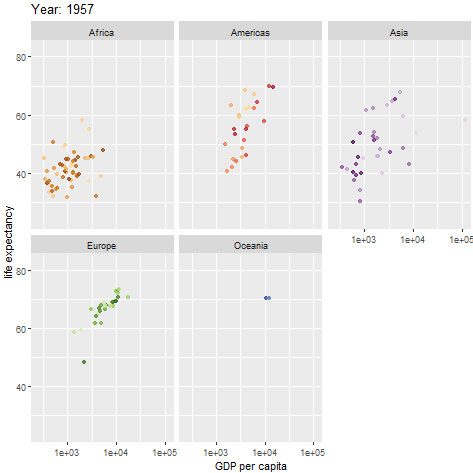
\includegraphics[width=0.3\textwidth]{image_reference/gganimate1.png}
        \label{fig:gganimate1}
    \end{subfigure}
    \begin{subfigure}
        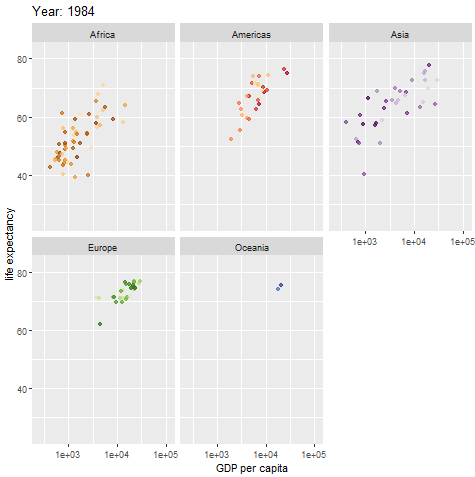
\includegraphics[width=0.3\textwidth]{image_reference/gganimate2.png}
        \label{fig:gganimate2}
    \end{subfigure}
    \begin{subfigure}
        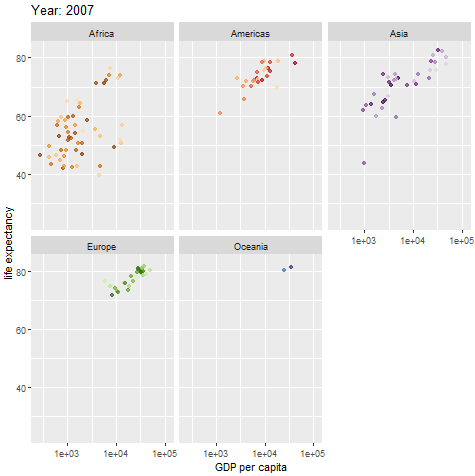
\includegraphics[width=0.3\textwidth]{image_reference/gganimate3.png}
        \label{fig:gganimate3}
    \end{subfigure}
    \caption{Screenshots of animated scatterplot at different time stamps}
    \label{fig:overall}
\end{figure}

\noindent The animated scatter plots provide a dynamic visualisation of the relationship between GDP per capita and life expectancy in each country over time. The animation is displayed across 5 separate animated scatter plot, each grouping the data from countries from a specific continent to reduce clutter and cognitive load. This animation helps in understanding temporal trends and patterns in the data that may not be apparent in static plots.\\

\noindent The conclusions drawn from the animated plots differ from those of the static plot. For instance, while the static plot suggests a general positive correlation between GDP per capita and life expectancy, the animated plots reveal nuances such as the pace of improvement in life expectancy over time, variations in the relationship between different countries and continents, and the impact of historical events or economic changes on life expectancy trends. In general, the animated plots offer a richer and more dynamic exploration of the data, leading to potentially deeper insights and understanding.

\subsection{Bubble Charts}
\subsubsection{Theory of Bubble Charts}
\noindent Bubble charts are a captivating data visualisation tool that extend beyond the typical two-dimensional scatter plot by introducing an extra dimension. They represent data points as bubbles or circles on a two-dimensional plane, where the size of each bubble encodes a third variable.\\

\noindent The construction of bubble charts, is parallel to that of a scatter plot, but involves the scaling the data values to determine the size of each bubble. While it isn't always the case, the size of these is typically proportional to the variable it represents. The choice of scaling method depends on the data distribution and the message the chart aims to convey.\\

\noindent Generally, the formula for calculating the bubble radius (\(R)\) involves applying the scaling function
\[
R = kV,
\]
\noindent where \(R\) represents the size of the bubble, \(V\) the value of the variable being represented, and \(k\) a scaling factor to control the bubble size. Selecting an appropriate scaling factor (\(k\)) is critical for maintaining the proportionality between the bubble size and the variable being represented.\\ 

\noindent Hence, bubble chart represents data points in three dimensions: x-coordinate, y-coordinate, and bubble size. Each data point is denoted by a triplet of values \((x_i, y_i, C_i)\), where \(x_i\) and \(y_i\) represent the coordinates, and \(C_i\) is the equation of the circle for the \(i\)-th observation. In the context of a bubble chart, the radius \(R_i\) of each bubble is expressed as \(k \cdot V_i\), allowing us to formulate the equation for each circle as:

\[
(x - x_i)^2 + (y - y_i)^2 = (kV_i)^2, 
\]

\noindent where \(x_i\) and \(y_i\) denote the coordinates of the circle's center.\\

\noindent Since each bubble \(B_i\) can be defined mathematically by the triplet \((x_i, y_i, C_i)\), akin to the scatter plot, the bubble plot can be described as a set of ``bubbles" \( \{B_1, \ldots, B_n\}\), where \(n\) represents the number of observations in the set.

\subsubsection{Bubble Charts in Practice}\\

\noindent The bubble chart shown in Figure~\ref{fig:bubble-plot}, as the scatter plots in Figure~\ref{fig:bubble-plot-construction}, visualises data from the mtcars dataset. The single bubble charts depicts the relationship between car models and their fuel efficiency (mpg) while using the size of the bubbles to represent the car's horsepower (hp), and even colour-coding the bubbles based on the number of cylinders (cyl).\\

\begin{knitrout}\scriptsize
\definecolor{shadecolor}{rgb}{0.969, 0.969, 0.969}\color{fgcolor}\begin{figure}[H]

{\centering 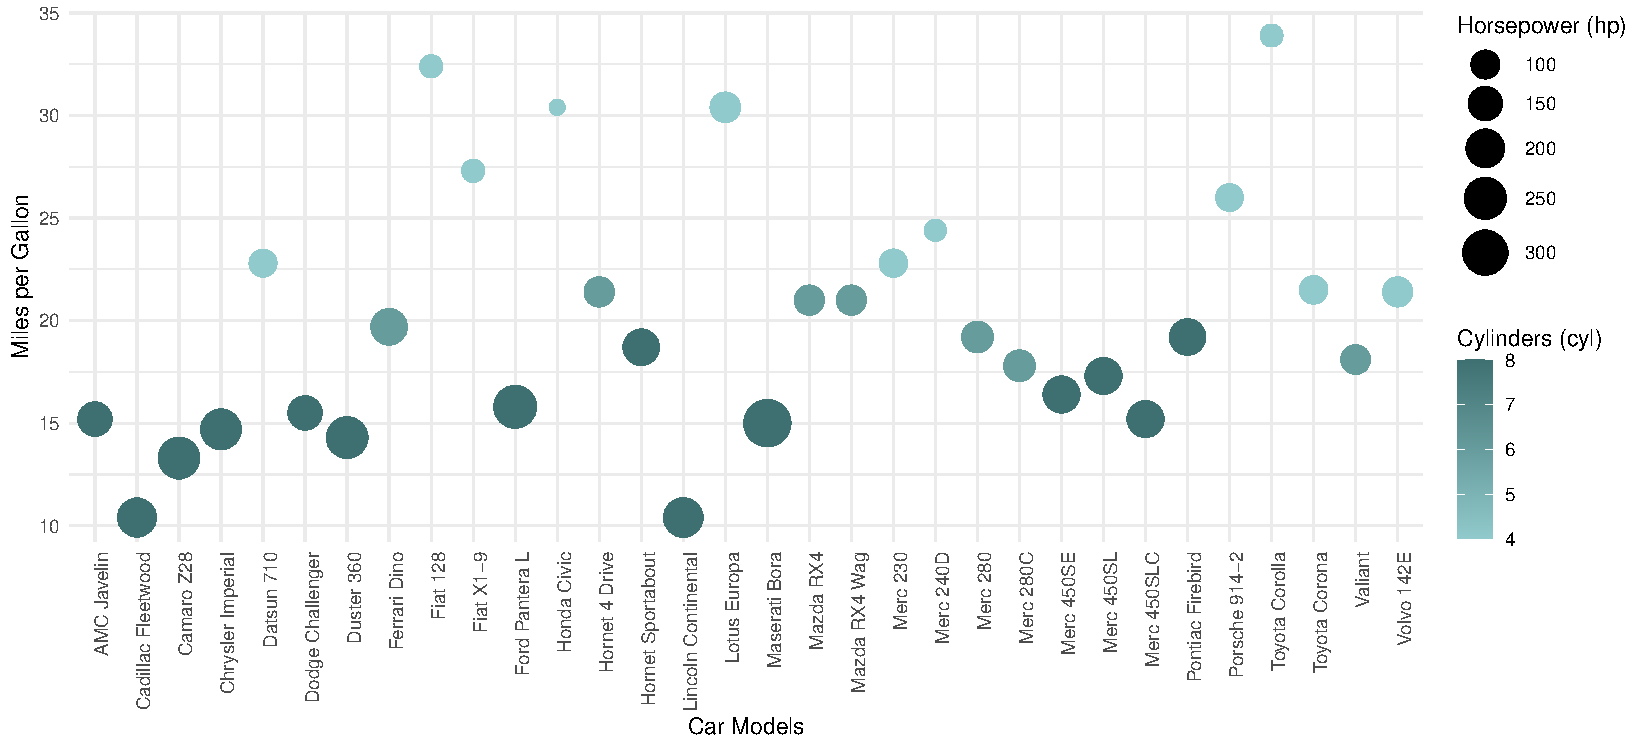
\includegraphics[width=\maxwidth]{figure/beamer-bubble-plot-1} 

}

\caption[Bubble plot illustrating trends in car types and performance]{Bubble plot illustrating trends in car types and performance}\label{fig:bubble-plot}
\end{figure}

\end{knitrout}

\\\noindent In Figure~\ref{fig:bubble-plot} a strong correlation between the cars' number of cylinder and their horsepower can be quickly identified. This is due to the fact that as size of the dots (representing horsepower) increases, their colour (representing the number of cylinders) simultaneously becomes darker. Furthermore, a correlation between the miles per gallon consumed by the different types of cars and their number of cylinders and horsepower is easily identifiable in Figure~\ref{fig:bubble-plot}. This is shown by the fact that, in the same way that the darker dots cluster towards the bottom of the graph and become lighter as they reach the top of the graph, those with a large diameter also cluster near the lower part and decrease in size as they ascend. \\ 

\noindent 
The efficiency of bubble charts is highlighted by the fact that capturing just some of the information provided by this single bubble chat - that is, the information regarding the car models, the miles covered per gallon, and the horsepower of each of these, requires three different scatter plots. These are displayed in Figure~\ref{fig:bubble-plot-construction}. The contrast between the simplicity and readability of Figure~\ref{fig:bubble-plot}, and the density and complexity of Figure~\ref{fig:bubble-plot-construction} emphasises the advantages of bubble charts in representing datasets with a higher number of variables. 


\subsection{Simple Linear Regression}
\\Regression models are statistical tools that provide functions to estimate the relationship between the response variable and one or more explanatory variables. Regression analysis is widely adopted by data scientists, who use large datasets to build predictive models for trend forecasting. The fol- lowing paragraphs will introduce simple linear regression models and demonstrate their usage using the mtcars dataset.

\subsubsection{Theory of Simple Linear Regression} 

\\Let $\mathbf{x} = (x_1, \dots, x_n)^T$ denote $n$ explanatory variables and let $\mathbf{Y} = (Y_1, \dots, Y_n)^T$ denote $n$ corresponding response variables.
\\  
\\In a simple linear model, it is assumed that the response variables $Y_1, \dots, Y_n$ are uncorrelated with a common variance $\sigma^2$, and their expectations are given by $E(Y_i| x_i) = \beta_0 + \beta_1 x_i$. The expectations \index{Simple linear regression!expectations}generated by $\beta_0$ and $\beta_1$ given $x_i$ can be expressed as:

\begin{equation}\label{eq:4-1}
\mathrm{E}(\mathbf{Y} | \mathbf{x}) =
\left( \begin{array}{ccc}
\beta_0+\beta_1 x_1\\
\vdots\\
\beta_0+\beta_1 x_n
\end{array} \right) = 
\left( \begin{array}{ccc}
1\\
\vdots\\
1
\end{array} \right) \beta_0 + 
\left( \begin{array}{ccc}
x_1\\
\vdots\\
x_n
\end{array} \right) \beta_1 =
\mathbf{1}_n \beta_0 + \mathbf{x} \beta_1 ,
\end{equation}
\\
\noindent
where $\mathbf{1}_n$ is an n-vector of 1's.
\\  
\\Given design matrix $\mathbf{X}$ where $\mathbf{x}_i = (1, x_i)$ and $\mathbf{\beta} = (\beta_0, \beta_1)^T$, then $E(Y_i|x_i) = \mathbf{x}_i \beta$. These assumptions can be equivalently written in the vector form:

\begin{equation}\label{eq:4-2}
\mathrm{E}(\mathbf{Y} | \mathbf{x}) = 
\left( \begin{array}{cc}
1 & x_1\\
\vdots& \vdots\\
1 & x_n
\end{array} \right) 
\left( \begin{array}{cc}
\beta_0 \\
\beta_1
\end{array} \right) = \mathbf{X} \boldsymbol{\beta}, \quad 
\text{var}(\mathbf{Y} | \mathbf{x}) =
\begin{pmatrix}
\sigma^2 & 0 & \cdots & 0 \\
0 & \sigma^2 & \cdots & 0 \\
\vdots & \vdots & \ddots & \vdots \\
0 & 0 & \cdots & \sigma^2
\end{pmatrix} = \sigma^2 \mathbf{I}_n.
\end{equation}

\subsubsection{Theory of Least Squares Estimation\index{Simple linear regression!least squares estimation}}

\noindent The residual sum of squares (RSS) is a measure of the goodness of fit in a regression model, where residuals are the differences between the response variables $y_i$ and responses generated by the regression model $\mathrm{E}(\mathbf{Y}_i | \mathbf{x})$. In least squares estimation, the goal is to find values of parameters $\boldsymbol{\beta} = (\beta_0, \beta_1)^T$ to minimise the RSS, denoted by $\mathrm{Q}$: 

\begin{equation}\label{eq:4-3}
\mathrm{Q} = \sum_{i=1}^{n} [y_i - \mathrm{E} (Y_i | \mathbf{x})]^2 
           = [\mathbf{y}- \mathrm{E} (\mathbf{Y} | \mathbf{x})]^{T} [\mathbf{y}- \mathrm{E} (\mathbf{Y} | \mathbf{x})] 
           = (\mathbf{y}- \mathbf{X} \boldsymbol{\beta})^{T} (\mathbf{y}- \mathbf{X} \boldsymbol{\beta}),
\end{equation}

\noindent
where $\mathbf{y}$ is n-vector of response variables and $\mathbf{X}$ is the $n \times 2$ design matrix. The partial derivative of $Q$ with respect to vector $\boldsymbol{\beta}$ is:

\begin{equation}\label{eq:4-4}
\frac{\partial Q}{\partial \boldsymbol{\beta}} = 2(\mathbf{X}^T\mathbf{X} \boldsymbol{\beta} - \mathbf{X}^T\mathbf{y}),
\end{equation}

\noindent
Equating $\frac{\partial Q}{\partial \boldsymbol{\beta}} = \mathbf{0}$, the vector $\hat{\boldsymbol{\beta}}$, the least squares estimate of $\boldsymbol{\beta}$, can be written as:

\begin{equation}\label{eq:4-5}
\mathbf{X}^T(\mathbf{y}-\mathbf{X}\hat{\boldsymbol{\beta}})=\mathbf{0}.
\end{equation}

\noindent 
The least squares estimate of $\boldsymbol{\beta}$ is given by:
\begin{equation}\label{eq:4-6}
\hat{\boldsymbol{\beta}} = (\mathbf{X}^T\mathbf{X})^{-1}\mathbf{X}^T\mathbf{y}.
\end{equation}
\\ 
\noindent 
The least squares estimate $\hat{\boldsymbol{\beta}}$ is an unbiased estimator:

$$ \mathrm{E}(\hat{\boldsymbol{\beta}}) = \mathrm{E}((\mathbf{X}^T\mathbf{X})^{-1}\mathbf{X}^T\mathbf{y}) = (\mathbf{X}^T\mathbf{X})^{-1}\mathbf{X}^T\mathbf{X}\boldsymbol{\beta} = \boldsymbol{\beta}.
$$
\noident 
\subsubsection{Case Example: 1970s Automobiles}\\
\noindent In this section, we will study the performance of 1970s automobiles using the mtcars dataset, employing the method of linear regression. Performance is measured in Miles per Gallon (mpg); the higher the mileage, the more efficient the automobile. We will start with the visualisation of a simple linear regression model, followed by the discussion of linear regression models and the model selection method.

\noindent
\\In the preliminary stages of data exploration, calculating the correlation matrix is a crucial step before engaging in regression modeling, as shown in Figure~\ref{fig:cor-matrix-mtcars2}. In real-world scenarios, variables are often correlated, and entirely independent relationships are seldom encountered. Therefore, analysing pairwise correlations becomes essential. This helps in understanding multicollinearity issues within the model. Multicollinearity occurs when one covariate within the model can be accurately predicted from another covariate. When this happens, the coefficient estimates of the model can change unpredictably due to minor changes in the data.\\



\begin{knitrout}\scriptsize
\definecolor{shadecolor}{rgb}{0.969, 0.969, 0.969}\color{fgcolor}\begin{figure}[H]

{\centering 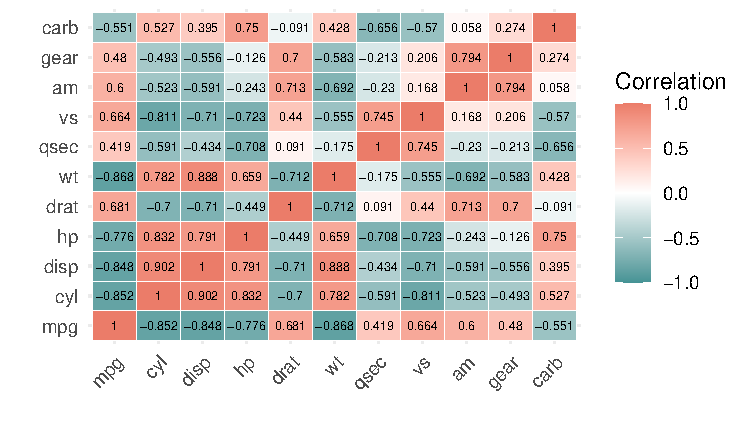
\includegraphics[width=\maxwidth]{figure/beamer-cor-matrix-mtcars2-1} 

}

\caption[Correlation matrix of all variables in mtcars dataset]{Correlation matrix of all variables in mtcars dataset}\label{fig:cor-matrix-mtcars2}
\end{figure}

\end{knitrout}

\noindent
For the simple linear regression model, the response variable is Miles per Gallon (mpg), and we select weight (wt) as the explanatory variable. Note that mpg and wt are highly correlated, with a correlation coefficient of -0.868. This suggests that wt may have strong predictive power for mpg. Use the R function \texttt{lm()} to calculate the linear regression model, with the summary displayed below.\\

\noindent
Observe that the t-test yields a p-value of $1.29 \times 10^{-10}$, which is less than $0.001$. This indicates that the variable wt holds high statistical significance in this model. For the fitted model, the slope is $\beta_1 = -5.3445$, meaning that for every increase of 1000 lbs, the car efficiency decreases by 5 miles per gallon. The RSS is 3.046. The simple linear regression line is displayed in Figure~\ref{fig:scatter-plot}.

\begin{knitrout}\scriptsize
\definecolor{shadecolor}{rgb}{0.969, 0.969, 0.969}\color{fgcolor}\begin{kframe}
\begin{alltt}
\hlcom{# SUMMARY FOR SIMPLE LINEAR REGRESSION, WITH RESPONSE VARIABLE MILES PER GALLON}
\hlstd{Modelwt} \hlkwb{<-} \hlkwd{lm}\hlstd{(}\hlkwc{formula} \hlstd{= mpg} \hlopt{~} \hlstd{wt,} \hlkwc{data} \hlstd{= mtcars)}
\hlkwd{summary}\hlstd{(Modelwt)}
\end{alltt}
\begin{verbatim}
## 
## Call:
## lm(formula = mpg ~ wt, data = mtcars)
## 
## Residuals:
##     Min      1Q  Median      3Q     Max 
## -4.5432 -2.3647 -0.1252  1.4096  6.8727 
## 
## Coefficients:
##             Estimate Std. Error t value Pr(>|t|)    
## (Intercept)  37.2851     1.8776  19.858  < 2e-16 ***
## wt           -5.3445     0.5591  -9.559 1.29e-10 ***
## ---
## Signif. codes:  0 '***' 0.001 '**' 0.01 '*' 0.05 '.' 0.1 ' ' 1
## 
## Residual standard error: 3.046 on 30 degrees of freedom
## Multiple R-squared:  0.7528,	Adjusted R-squared:  0.7446 
## F-statistic: 91.38 on 1 and 30 DF,  p-value: 1.294e-10
\end{verbatim}
\end{kframe}
\end{knitrout}

\begin{knitrout}\scriptsize
\definecolor{shadecolor}{rgb}{0.969, 0.969, 0.969}\color{fgcolor}\begin{figure}[H]

{\centering 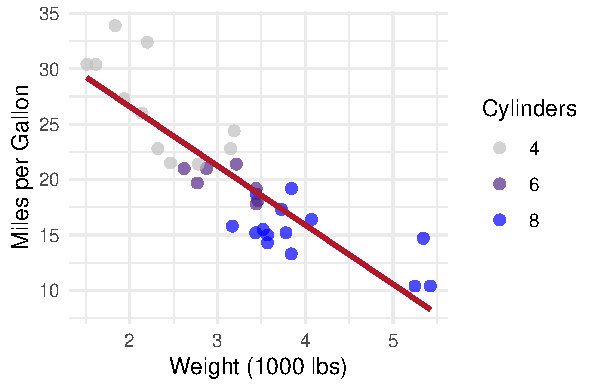
\includegraphics[width=\maxwidth]{figure/beamer-scatter-plot-1} 

}

\caption[Scatter plot of car weights vs MPG]{Scatter plot of car weights vs MPG}\label{fig:scatter-plot}
\end{figure}

\end{knitrout}

\subsection{LOESS Regression}
\noindent
Locally weighted scatterplot smoothing (LOWESS) is a local regression method for a response variable $Y$ on a single predictor $X$. LOWESS was proposed by William S. Cleveland in 1979, it is the special case to higher dimention locally estimated scatterplot smoothing (LOESS) regression method. They are non-parametric regression methods that fits a linear regression model for each neighbourhood of data. Unlike GLM, the LOESS model does not provide a global function to fit the data; rather, it fits neighborhoods of the data.

\subsubsection{Theory of LOESS Regression}

\noindent
Suppose we have $n$ ordered observations $\{(x_1,y_1), \dots, (x_n,y_n)\}$ with predictors $x_i$ and response variables $y_i$. Assume a model of the form

$$y_i = g(x_i) +  \varepsilon_i,$$
\noindent
where $\mathrm{g}$ is an unknown smooth function and $\varepsilon_i$ is i.i.d.Gaussian error terms with mean $0$ and variance $\sigma^2$.\\

\noindent
Let $\Delta_i(x) = |x - x_i|$ represent the horizontal distance between $x$ and $x_i$. Let $\Delta_{(i)}(x)$ denote the ordered distances to $x$, arranged from smallest to largest.\\

\noindent
For each point $(x,y)$ consider the neighbourhood to fit a line segment around it. The size of the neighbourhood indicates the number of data points used to fit the line segments and is determined by the smoothing parameter $\alpha$. For $\alpha \leq 1$, each  neighbourhood consists of $\frac{n}{\alpha}$ number of points \cite{rloess}. Each point $(x_i, y_i)$ in the neighbourhood of point $(x,y)$ is assigned with a weight\index{LOESS!weight}, ``importance" of the data point to the line segment \cite{ytloess}. The weight of $(x_i,y_i)$ is denoted as $w_i(x)$, which is defined as:

\begin{equation}\label{eq:4-7}
w_i(x) = T(\Delta_i (x); \Delta _{(q)}(x)).
\end{equation}

\noindent
Tricube weight function $T(u,t)$ is defined as:
\begin{equation}\label{eq:4-8}
T(u;t) = \left\{
  \begin{array}{ll}
    (1-(u/t)^3)^3 & \text{for } 0 \leq u < t \\
    0 & \text{for } u \geq t \\
  \end{array}
\right, 
\end{equation}

\noindent
where $u$ is the horizontal distance between neighbourhood point of interest $(x_i,y_i)$ to point $(x,y)$ and $t$ is the maximum distance threshold. For points in the neighbourhood with horizontal distance exceeding threshold $t$, they are assigned with weight $0$ by the tricube weight function.\\

\noindent
For $\alpha > 1$, for each point $(x,y)$ the neighbourhood include all points. The maximum distance threshold is assumed to be $\alpha^{\frac{1}{p}}$, for $p$ explanatory variables. The weight is given by:

\begin{equation}\label{eq:4-9}
w_i(x) = T(\Delta_i (x); \Delta _{(n)}(x))\alpha.\\
\end{equation}

\noindent
The line segment is fitted by weighted least square, and this is the preliminary estimation\index{LOESS!preliminary estimation} $\hat{g}(x)$ for every point $(x,y)$.\\

\noindent
Both LOWESS and LOESS penalise \index{LOESS!penalty}the outliers in the preliminary estimation by assigning points further away from $\hat{g}(x)$ with less weight than before. The robustness weight \index{LOESS!robustness weight}(the adjusted weight) is given by:
$$r_i = B(\hat{\varepsilon}_i, 6\mathrm{m}),$$

\noindent
where bisquare weight function is defined as:

\begin{equation}\label{eq:4-10}
B(u;b) = \left\{
  \begin{array}{ll}
    (1-(u/b)^2)^2 & \text{for } 0 \leq |u| < b \\
    0 & \text{for } |u| \geq b \\
  \end{array},
\right
\end{equation}

\noindent
and the median absolute residual $\mathrm{m}$ is defined as $\mathrm{m} = \mathrm{median}(|\hat{\varepsilon}_i|)$, the residual $\hat{\varepsilon}_i$ is defined as $\hat{\varepsilon}_i = y_i - \hat{y}(x_i)$. \\

\noindent
Note the process of weight adjustment using previous estimation is iterated several times until a smooth curve is obtained.\\

\noindent
The updated model estimate $\hat{g}(x)$, is computed using the local fitting method, but with the neighborhood weights $w_i{(x)$ replaced by $r_i w_i(x)$ \cite{loess}.

\subsubsection{Case Example: Estate Price in Taipei}\\

\noindent
Property valuation can be modelled as a regression problem, in this analysis, we delve into the pricing of properties based on their age. Using the Taipei Housing dataset, we investigate the relationship between the age of houses (measured in years) and their prices (measured in New Taiwan dollars per unit area). Linear regression model and the LOESS regression model are used, as shown in Figure~\ref{fig:estate-data-plot}.\\

\noindent
The linear model has a residual standard error of 13.32, while the LOESS model has a residual standard error of 12.16. Cross-validation is a method to compare model goodness of fit. LOESS, with its ability to capture local variations may outperform linear regression, which minimises the least squares estimate $\hat{\beta}$.\\



\begin{knitrout}\scriptsize
\definecolor{shadecolor}{rgb}{0.969, 0.969, 0.969}\color{fgcolor}\begin{kframe}
\begin{alltt}
\hlcom{# LINEAR REGRESSION VS. LOESS MODEL}
\hlkwd{ggplot}\hlstd{(}\hlkwc{data} \hlstd{= estate,} \hlkwd{aes}\hlstd{(}\hlkwc{x} \hlstd{= house_age,} \hlkwc{y} \hlstd{= price_per_area))} \hlopt{+}
  \hlkwd{geom_point}\hlstd{(}\hlkwc{size} \hlstd{=}\hlnum{0.5}\hlstd{)} \hlopt{+}
  \hlkwd{theme_minimal}\hlstd{()}\hlopt{+}
  \hlkwd{scale_x_continuous}\hlstd{(}\hlkwc{labels} \hlstd{= scales}\hlopt{::}\hlkwd{number_format}\hlstd{(}\hlkwc{scale} \hlstd{=} \hlnum{1}\hlstd{))} \hlopt{+}
  \hlkwd{scale_y_continuous}\hlstd{(}\hlkwc{labels} \hlstd{= scales}\hlopt{::}\hlkwd{number_format}\hlstd{(}\hlkwc{scale} \hlstd{=} \hlnum{1}\hlstd{))} \hlopt{+}
  \hlkwd{geom_smooth}\hlstd{(}\hlkwc{method} \hlstd{=} \hlstr{"loess"}\hlstd{,} \hlkwc{se} \hlstd{=} \hlnum{FALSE}\hlstd{,} \hlkwc{color} \hlstd{=} \hlstr{"#EB7C69"}\hlstd{,} \hlkwc{span} \hlstd{=} \hlnum{0.5}\hlstd{)} \hlopt{+}
  \hlkwd{geom_smooth}\hlstd{(}\hlkwc{method} \hlstd{=} \hlstr{"lm"}\hlstd{,} \hlkwc{se} \hlstd{=} \hlnum{FALSE}\hlstd{,} \hlkwc{color} \hlstd{=} \hlstr{"#459395"}\hlstd{,} \hlkwc{formula} \hlstd{= y} \hlopt{~} \hlstd{x)} \hlopt{+}
  \hlkwd{labs}\hlstd{(}\hlkwc{title} \hlstd{=} \hlstr{"House Age vs. House Price"}\hlstd{,}
       \hlkwc{x} \hlstd{=} \hlstr{"house age (year)"}\hlstd{,}
       \hlkwc{y} \hlstd{=} \hlstr{"price (unit area)"}\hlstd{)} \hlopt{+}
  \hlkwd{theme_minimal}\hlstd{()}
\end{alltt}
\end{kframe}\begin{figure}[H]

{\centering 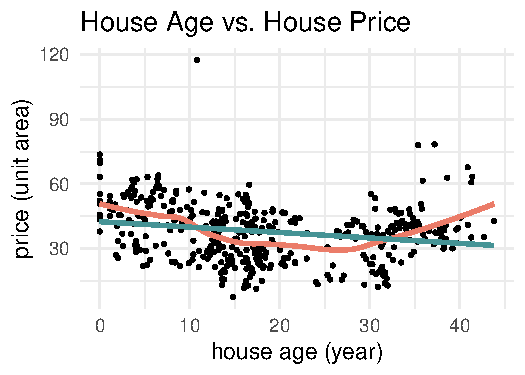
\includegraphics[width=\maxwidth]{figure/beamer-estate-data-plot-1} 

}

\caption[Estate valuation using house age, linear regression and smooth regression methods]{Estate valuation using house age, linear regression and smooth regression methods}\label{fig:estate-data-plot}
\end{figure}

\end{knitrout}

\subsubsection*{Chapter Overview and Further Reading References}

\noindent This chapter delves into the theory of scatter plots, and bubble charts, as well as simple linear regression and LOESS regression. These concepts are firmly established the existing statistical literature. Further insights into scatter plots and bubble charts can be found in Leland Wilkinson's \href{https://link.springer.com/chapter/10.1007/978-3-642-21551-3_13}{\textit{The Grammar of Graphics}} (2005), while comprehensive details on simple linear regression theory are available in \href{https://blackwells.co.uk/bookshop/product/Introduction-to-Linear-Regression-Analysis-by-Douglas-C-Montgomery-Elizabeth-A-Peck-G-Geoffrey-Vining/9781119578727}{\textit{Introduction to Linear Regression Analysis}} (2021) by Douglas C. Montgomery, Elizabeth A. Peck, and G. Geoffrey Vining. Additionally, \href{https://www.taylorfrancis.com/books/edit/10.1201/9780203738535/statistical-models-hastie}{\textit{Local Regression Models}} (1992) by William S. Cleveland, Eric Grosse, and William M. Shyu offers an in-depth exploration of LOESS regression theory.

\newpage

\section{Visualising Beyond Two Dimensions} 

\noindent This chapter extends beyond the realm of two dimensional data visualisations. Within this chapter, advanced techniques are explored to unravel complex relationships involving multiple variables \cite{ward2010interactive}. The Principal Component Analysis (PCA) is introduced as a powerful method for dimensionality reduction, enabling a concise representation of high-dimensional datasets. Multiple innovative methods involving the visualisation of high-dimensional data in lower-dimensional space such as biplots, principal curves, and t-distributed Stochastic Neighbor Embedding (t-SNE) are studied. 

\subsection{Principal Component Analysis (PCA)}

\subsubsection{Theory of PCA}
\noindent
Principal Component Analysis (PCA) is one of the most widely-used dimensionality reduction techniques. The basic idea is to use the dependencies between the variables to project the data into a low-dimensional subspace, without losing too much information.\\

\noindent
The feature matrix $\mathbf{X}$ is an $N \times D$ real-valued matrix:
$$\mathbf{X} = \left( \begin{array}{ccc}
    \mathbf{x}^{T}_{1}\\
    \vdots\\
    \mathbf{x}^{T}_{n}
    \end{array} \right) = \begin{pmatrix}
x_{1,1} & x_{1,2} & \cdots & x_{1,D} \\
 &\vdots & & \\
x_{N,1} & x_{N,2} & \cdots & x_{N,D}
\end{pmatrix},$$
\noindent
with $N$ observations and $D$ variables (also known as features).\\

\noindent
Define a linear and orthogonal mapping $\mathbf{W}: \mathbf{x} \to \mathbf{z}$, acting as a 'transformer' between observation $\mathbf{x}$ and its low-dimensional projection $\mathbf{z}$. The matrix $\mathbf{W}$ is a $D \times L$ orthogonal and normalised matrix, where its column vectors are represented as $\mathbf{W} = [\mathbf{w}_1, \dots, \mathbf{w}_L]$. Then, for all $i \neq j$, $\mathbf{w}_i \mathbf{w}_j = 0$ and $\mathbf{w}_i^T \mathbf{w}_i = 1$. This matrix allows for the projection of data from its original high-dimensional space to the low-dimensional subspace using $\mathbf{z} = \mathbf{W}^T\mathbf{x}$, known as encoding. To reconstruct $\mathbf{x}$ from $\mathbf{z}$, $\hat{\mathbf{x}} = \mathbf{W}\mathbf{z}$ will give the high-dimensional approximation of the observation, this process is known as decoding.\\

\noindent
The optimal solution of PCA is obtained by minimising the loss function\index{Principal component analysis!loss function}, which represents the reconstruction error \index{Principal component analysis!reconstruction error}subject to constraint $\mathbf{W}$. The loss function is defined as follows:

\begin{equation}
\mathcal{L}(\mathbf{W}) = \frac{1}{N}\sum_{n=1}^{N}||\mathbf{x}_n - \hat{\mathbf{x}}||^2_2.
\end{equation}

\subsubsection{Derivation of PCA}

In general, the vector $\mathbf{w}_i$ is given by the equation $\mathbf{\Sigma} \mathbf{w}_i = \lambda \mathbf{w}_i$, where $\mathbf{\Sigma}$ is the covariance matrix and $\lambda$ is the $i^{th}$ largest eigenvalue of $\mathbf{\Sigma}$, for $i = 1, \dots, L$.\\

\noindent
Define the covariance matrix \index{Principal component analysis!covariance matrix}$\mathbf{\Sigma} = \frac{1}{N} \sum_{n=1}^N(\mathbf{x}_n-\bar{\mathbf{x}})(\mathbf{x}_n-\bar{\mathbf{x}})^T$. Without loss of generality, let's assume that all observations in matrix $\mathbf{X}$ are centred around $0$ mean, then $\bar{\mathbf{x}} = 0$. The covariance matrix can be written in a simple form:

\begin{equation}
\mathbf{\Sigma} = \frac{1}{N} \sum_{n=1}^N\mathbf{x}_n\mathbf{x}_n^T = \frac{1}{N} \mathbf{X}\mathbf{X}^T. \label{eq:cov}
\end{equation}

\noindent
The optimal encoding \index{Principal component analysis!optimal encoding}$\mathbf{Z}$ ensures minimum information loss when data is projected to a lower-dimensional subspace. To determine this optimal encoding, we minimise the reconstruction error with respect to $\mathbf{w}$ and $\mathbf{z}$.

\begin{equation}
\begin{aligned}
\mathcal{L}(\mathbf{w},\mathbf{z}) &= \frac{1}{N}\sum ||\mathbf{x}_n - \mathbf{W}\mathbf{z}_n||^2  \\
&= \frac{1}{N}\sum (\mathbf{x}_n - \mathbf{W}\mathbf{z}_n)^T(\mathbf{x}_n - \mathbf{W}\mathbf{z}_n)  \\
&= \frac{1}{N}\sum \mathbf{x}_n^T\mathbf{x}_n - 2\mathbf{x}_n^T\mathbf{W}\mathbf{z}_n+\mathbf{z}_n^T\mathbf{W}^T\mathbf{W}\mathbf{z}_n . \label{eq:lossfunc}
\end{aligned}
\end{equation}

\noindent
To determine the optimal encoding $\mathbf{z}_n$ for the $n^{th}$ observation, we set the derivative with respect to $\mathbf{z}_n $ equal to $0$:

$$\frac{\partial \mathcal{L}(\mathbf{w},\mathbf{z})}{\partial \mathbf{z}_n} = \frac{1}{N} (-2 \mathbf{x}_n^T\mathbf{W} + 2\mathbf{z}_n)= \mathbf{0}.$$

\noindent
Thus we find that $\mathbf{z}_n = \mathbf{W}^T\mathbf{x}_n$ yields the optimal encoding for the $n^{th}$ observation.\\

\noindent
Next, we aim to find the matrix $\mathbf{W}$ which gives the optimal encoding. We start by expanding and simplifying the loss function \index{Principal component analysis!loss function}$\mathcal{L}(\mathbf{W})$ from equation \ref{eq:lossfunc}: \\

\begin{equation}
\mathcal{L}(\mathbf{W}) = \frac{1}{N} \sum_{n=1}^{W}\mathbf{x}_n^T\mathbf{x}_n - \sum_{n=1}^{L}\mathbf{W}_l^T(\frac{1}{N} \sum_{n=1}^{N}\mathbf{x}_n\mathbf{x}_n^T)\mathbf{W}_l.
\end{equation}

\noindent
WLOG, our data is assumed to be centred around $0$ mean (by \ref{eq:cov}), the loss function can be represented as:

\begin{equation}
\mathcal{L}(\mathbf{W}) = \mathrm{constant} - \sum_{l=1}^L\mathbf{W}_l^T\mathbf{\Sigma}\mathbf{W}_l.
\end{equation}

\noindent 
Since $\mathbf{W}$ is a normalised matrix, it has the property $\mathbf{W}_i^T\mathbf{W}_i =1$ for all $i =1, \dots, N$. Therefore, when computing the partial derivative of $\mathcal{L}(\mathbf{W})$ with respect to vector $\mathbf{w}_1$, we can apply the Lagrange multipliers to $\mathcal{L}(\mathbf{w}_1)$ and calculate the derivative of $\hat{\mathcal{L}}(\mathbf{w}_1)$ instead:

\begin{equation}
\hat{\mathcal{L}}(\mathbf{w}_1) = - \mathbf{w}_1^T\mathbf{\Sigma}\mathbf{w}_1 + \lambda(\mathbf{w}_1^T\mathbf{w}_1 -1),
\end{equation}

\noindent 
Equating $\frac{\partial \hat{\mathcal{L}}(\mathbf{w}_1))}{\partial \mathbf{w}_1} = \mathbf{0}$, the weight vector $\mathbf{w}_1$ which minimise the loss function can be expressed as \cite{pcaformula}:

\begin{equation}
\frac{\partial \hat{\mathcal{L}}(\mathbf{w}_1))}{\partial \mathbf{w}_1} = 2\mathbf{\Sigma}\mathbf{w}_1+2\lambda \mathbf{w}_1 = \mathbf{0}.
\end{equation}

\noindent 
Therefore $\mathbf{\Sigma}\mathbf{w}_1 = \lambda \mathbf{w}_1$ that is, $\mathbf{w}_1$ is the eigenvector of $\mathbf{\Sigma}$ with eigenvalue $\lambda$.\\

\noindent 
Premultiply by $\mathbf{w}_1^T$, $\mathbf{w}_1^T\mathbf{\Sigma}\mathbf{w}_1 = \lambda \mathbf{w}_1^T\mathbf{w}_1 = \lambda$. To minimise the loss $\mathcal{L}}(\mathbf{w}_1)$ we maximise $\mathbf{w}_1^T\mathbf{\Sigma}\mathbf{w}_1$. Thus the largest eigenvalue $\lambda$ would minimise the loss $\mathcal{L}}(\mathbf{w}_1)$.\\

\noindent 
Adopting the same methodology, the second largest eigenvalue $\lambda$_2$ would minimise the loss $\mathcal{L}}(\mathbf{w}_2)$.\\

\noindent 
Therefore, order the eigenvectors by their corresponding eigenvalues $\{\mathbf{w}_1, \dots, \mathbf{w}_L\}$. These form the columns of the weight matrix $\mathbf{W} \in \mathbb{R}^{D \times L}$ \cite{ml}.\\

\subsection{Biplots}
\noindent 
A biplot is a graphical representation that neatly captures the relationships between variables and observations in a reduced-dimensional space defined by the principal components. Biplots facilitate the exploration of complex multivariate data by providing a simultaneous display of both samples (observations) and variables in a single plot. They are commonly understood to be a "generalisation of the simple two-variable scatterplot".\\

\noindent At their core, biplots offer a graphical representation of a standardised data matrix, whose rows \(n\) are the samples, and whose columns \(p\) are the variables, by projecting these onto a two-dimensional plane. To do this, mathematical computations derived from techniques like Singular Value Decomposition (SVD) and Principal Component Analysis (PCA) are required.\\

\noindent In recent years, there have been substantial developments in biplots \cite{gower1995biplots}. The technique has expanded far beyond what is now referred to as the ``classical biplots" or ``PCA biplots". However, this section studies the foundations of this visualisation technique, and thus, the emphasis is on biplots within the framework of PCA.

\subsubsection{Construction of PCA Biplots}

\noindent \textbf{Singular Value Decomposition\index{Biplots!singular value decomposition}}\\
\noindent Principal component biplots are based on singular value decomposition of the $(n \times p)$ data matrix $\mathbf{X}$ of $n$ observations on $p$ variables with rank $r$. The singular value decomposition of the standardised matrix $\mathbf{X}$ is defined to be the following:

\[\mathbf{X} = \mathbf{U}\mathbf{B}\mathbf{S}^{T}, \]

\noindent where $\mathbf{U}$ is an $(n \times r)$ orthogonal matrix, and $\mathbf{S}$ is an $(p \times r)$ orthogonal matrix. The columns of $\mathbf{U}$ and $\mathbf{S}$ are the left and right singular vectors. $\mathbf{B}$ is a $(r \times r)$ diagonal matrix with entries $b_1, \ldots, b_r$ such that $b_1 \geq \dots b_r \geq 0$ \cite{jolliffe2003principal}. These entries, known as the singular values play a key role in the generation of biplots which is discussed later on.\\

\noindent In order to find this singular value decomposition, firstly we require the computation of the orthogonal diagonalisation  

\[
\mathbf{X}^T\mathbf{X}=\mathbf{PDP}^T,
\] 

\noindent where $\mathbf{D}$ is the diagonal matrix of eigenvalues of $\mathbf{X}^T\mathbf{X}$ and $\mathbf{P}$ is an orthogonal matrix composed of the normalised eigenvectors of $\mathbf{X}^T\mathbf{X}$.\\

\noindent With this, the matrices $\mathbf{B}$ and $\mathbf{S}$ are computed. Matrix $\mathbf{S}$ is equivalent to the matrix $\mathbf{P}$ previously calculated, and matrix $\mathbf{B}$ is a $(n \times p)$ diagonal matrix, where the diagonal entries are the ``singular values" \index{Biplot!singular values}with any additional rows and columns of zero to make the dimensions of $\mathbf{B}$ match those of $\mathbf{X}$. The singular values referenced are the square roots of the eigenvalues of $\mathbf{X}^T\mathbf{X}$. Hence matrix $\mathbf{B}$ is of the form

\[
\mathbf{B} = 
\begin{bmatrix}
    \mathbf{D}^{\frac{1}{2}} & \mathbf{0} \\
    \mathbf{0} & \mathbf{0} \\
\end{bmatrix}.
\]

\noindent Finally, the $\mathbf{U}$ orthogonal matrix is calculated. The $i$-th column of $\mathbf{U}$ is given by

\[
\mathbf{u}_i = \frac{1}{\sigma_1}\mathbf{X}\mathbf{s}_i,
\]

\noindent where $\sigma_i$ are the singular values, and $\mathbf{s}_i$ are the columns of the matrix $\mathbf{S}$ \cite{baker2005singular}.\\

\noindent \textbf{PCA Biplot Construction}\\
\noindent Now, the heuristic argument motivating PCA biplots is the following. Define $\mathbf{B}^{\alpha}$, for $0 \leq \alpha \leq 1$, as a diagonal matrix who's diagonal elements are $b_1^{\alpha}, \ldots, b_r^{\alpha}$. The definition for $\mathbf{B}^{1-\alpha}$ is similar \cite{biplotsnotes}. Then, with the decomposition of matrix $\mathbf{X}$ found through SVD, the data can be further rewritten as
\[\mathbf{X} = \mathbf{U}\mathbf{B}^{\alpha}\mathbf{B}^{1-\alpha}\mathbf{S}^{T} = \mathbf{U}\mathbf{B}\mathbf{S}^{T} = \mathbf{G}\mathbf{H}^{T},\]

\noindent where \[\mathbf{G} = [\mathbf{g}_1, \dots , \mathbf{g}_n] = \mathbf{U}\mathbf{B}^\alpha, \quad \mathbf{H}^T = [\mathbf{h}_1, \dots , \mathbf{h}_p]^T = \mathbf{B}^{1-\alpha}\mathbf{S}^T. \]

\noindent Hence, the $i$th observation of the $j$th variable can be rewritten as

\[ x_{ij} = \mathbf{g}_i^T \mathbf{h}_j. \]

\noindent Both the $\mathbf{g}_i$ and $\mathbf{h}_j$ have $r$ elements, and hence, if $\mathbf{X}$ has rank 2, all could be plotted as points in two-dimensional space \cite{biplotsnotes}. Note that for the more general case, where $r > 2$, $x_{ij}$ can be written as

\[
x_{ij} = \sum_{k=1}^{r} u_{ik}b_{k}s_{jk}
\]

\noindent which is often well approximated by

\[
_m\tilde{x}_{ij} = \sum_{k=1}^{m} u_{ik}b_{k}s_{jk}, \quad \text{with } m < r.
\]

\noindent But this can be written
\[
_m\tilde{x}_{ij} = \sum_{k=1}^{m} \mathbf{g}_{ik}\mathbf{h}_{jk} = \mathbf{g}_{i}^{*T}\mathbf{h}_{j}^{*},
\]

\noindent where $\mathbf{g}^*_{i}, \mathbf{h}^*_{j}$ contain the first $m$ elements of $\mathbf{g}_i$ and $\mathbf{h}_j$ respectively. Hence, suggesting that if instead of using the $\mathbf{g}_i$ and the $\mathbf{h}_j$, we can just use their first elements (say, 2), respectively denoted by  $\mathbf{g}_{i}^{*}$  and  $\mathbf{h}_{j}^{*}$, to get

\[ x_{ij} \approx \mathbf{g}_{i}^{*T}\mathbf{h}_{j}^{*}.\]

\noindent Thus, $\mathbf{g}_i$ and $\mathbf{h}_j$ should provide a reasonable two-dimensional approximation of the $n$ observations and the $p$ variables \cite{jolliffe2003principal}.\\

\subsubsection{Case Example: Vintage Cars' Attributes}

\noindent This section presents a comparative analysis of PCA biplots generated through two distinct methodologies: manual mathematical construction and use of R's in-built functions. The focus lies on elucidating the mathematical intricacies, exploring relations, and highlighting differences between the two approaches. The mtcars dataset will serve as a benchmark.\\

\noindent \textbf{Methodologies Discussion}\\
\noindent Traditionally, biplots are constructed manually through mathematical operations based on SVD discussed previously. However, with computational tools like R, in-built functions such as \texttt{prcomp()} and \texttt{biplot()} streamline the process, removing tidious mathematical intricacies, which becomes particularly interesting when working with larger datasets.\\

\noindent The manual construction, which results in the biplot shown in Figure~\ref{fig:PCAbiplot}, begins with data standardisation followed by SVD decomposition to obtain matrices representing row and column contributions to principal components. These matrices are then utilised to construct the biplot. Conversely, the in-built function approach employs R's \texttt{prcomp()} function for PCA and directly generates the biplot using \texttt{biplot()}, without the need for explicit mathematical operations. The product of this method is shown in Figure~\ref{fig:PCAbiplot}.

\begin{knitrout}\scriptsize
\definecolor{shadecolor}{rgb}{0.969, 0.969, 0.969}\color{fgcolor}\begin{kframe}
\begin{alltt}
\hlcom{#MANUAL CONSTRUCTION OF A BIPLOT IN R}
\hlcom{# Standardise the data}
\hlstd{scaled_data} \hlkwb{<-} \hlkwd{scale}\hlstd{(mtcars)}

\hlcom{# Set the alpha parameter for SVD}
\hlstd{alpha} \hlkwb{<-} \hlnum{0}

\hlcom{# Preprocess the data using SVD}
\hlstd{preprocess} \hlkwb{<-} \hlstd{scaled_data} \hlopt{-} \hlkwd{matrix}\hlstd{(}\hlkwd{colMeans}\hlstd{(scaled_data),} \hlkwc{nrow} \hlstd{=} \hlkwd{nrow}\hlstd{(scaled_data),}
                                   \hlkwc{ncol} \hlstd{=} \hlkwd{ncol}\hlstd{(scaled_data),} \hlkwc{byrow} \hlstd{=} \hlnum{TRUE}\hlstd{)}
\hlstd{svd_mtcars} \hlkwb{<-} \hlkwd{svd}\hlstd{(preprocess)}
\hlstd{U} \hlkwb{<-} \hlstd{svd_mtcars}\hlopt{$}\hlstd{u}
\hlstd{L} \hlkwb{<-} \hlkwd{diag}\hlstd{(svd_mtcars}\hlopt{$}\hlstd{d)}
\hlstd{A} \hlkwb{<-} \hlstd{svd_mtcars}\hlopt{$}\hlstd{v}

\hlcom{# Calculate G and H matrices}
\hlstd{G} \hlkwb{<-} \hlstd{U} \hlopt \hlstd{(L}\hlopt\hlstd{(alpha))}
\hlstd{H} \hlkwb{<-} \hlkwd{t}\hlstd{((L}\hlopt \hlstd{(}\hlnum{1}\hlopt{-}\hlstd{alpha))} \hlopt \hlkwd{t}\hlstd{(A))}

\hlcom{# Extract the first two columns for biplot}
\hlstd{G2} \hlkwb{<-} \hlstd{G[,} \hlnum{1}\hlopt{:}\hlnum{2}\hlstd{]}
\hlstd{H2} \hlkwb{<-} \hlstd{H[,} \hlnum{1}\hlopt{:}\hlnum{2}\hlstd{]}

\hlcom{# Set up a side-by-side layout}
\hlkwd{par}\hlstd{(}\hlkwc{mfrow} \hlstd{=} \hlkwd{c}\hlstd{(}\hlnum{1}\hlstd{,} \hlnum{2}\hlstd{))}

\hlcom{# Create a biplot-like plot for manual construction with title}
\hlkwd{plot}\hlstd{(G2,} \hlkwc{xlim} \hlstd{=} \hlkwd{c}\hlstd{(}\hlopt{-}\hlnum{0.25}\hlstd{,} \hlnum{0.4}\hlstd{),} \hlkwc{xlab} \hlstd{=} \hlstr{"PC1"}\hlstd{,} \hlkwc{ylab} \hlstd{=} \hlstr{"PC2"}\hlstd{,} \hlkwc{main} \hlstd{=} \hlstr{"Manual Mathematical Construction"}\hlstd{)}

\hlkwd{par}\hlstd{(}\hlkwc{new} \hlstd{=} \hlnum{TRUE}\hlstd{)}
\hlkwd{plot}\hlstd{(H2,} \hlkwc{xlim} \hlstd{=} \hlkwd{c}\hlstd{(}\hlopt{-}\hlnum{4.5}\hlstd{,} \hlnum{8}\hlstd{),} \hlkwc{ylim} \hlstd{=} \hlkwd{c}\hlstd{(}\hlopt{-}\hlnum{4.5}\hlstd{,} \hlnum{8}\hlstd{),} \hlkwc{col} \hlstd{=} \hlstr{"#EB7C69"}\hlstd{,}
     \hlkwc{xaxt} \hlstd{=} \hlstr{"n"}\hlstd{,} \hlkwc{yaxt} \hlstd{=} \hlstr{"n"}\hlstd{,} \hlkwc{xlab} \hlstd{=} \hlstr{""}\hlstd{,} \hlkwc{ylab} \hlstd{=} \hlstr{""}\hlstd{)}
\hlkwa{for} \hlstd{(i} \hlkwa{in} \hlnum{1}\hlopt{:}\hlkwd{ncol}\hlstd{(scaled_data)) \{}
  \hlkwd{lines}\hlstd{(}\hlkwd{c}\hlstd{(}\hlnum{0}\hlstd{, H2[i,} \hlnum{1}\hlstd{]),} \hlkwd{c}\hlstd{(}\hlnum{0}\hlstd{, H2[i,} \hlnum{2}\hlstd{]),} \hlkwc{col} \hlstd{=} \hlstr{"#EB7C69"}\hlstd{,} \hlkwc{lwd} \hlstd{=} \hlnum{1.5}\hlstd{)}
\hlstd{\}}

\hlkwd{axis}\hlstd{(}\hlnum{3}\hlstd{)}
\hlkwd{axis}\hlstd{(}\hlnum{4}\hlstd{)}

\hlcom{#GENERATION OF A BIPLOT WITH R'S BUILT-IN FUNCTIONS}
\hlcom{# Standardise the data}
\hlstd{scaled_data} \hlkwb{<-} \hlkwd{scale}\hlstd{(mtcars)}

\hlcom{# Perform Principal Component Analysis (PCA)}
\hlstd{pca_result} \hlkwb{<-} \hlkwd{prcomp}\hlstd{(scaled_data,} \hlkwc{scale.} \hlstd{=} \hlnum{TRUE}\hlstd{)}

\hlcom{# Create a biplot with title}
\hlkwd{biplot}\hlstd{(pca_result,} \hlkwc{cex} \hlstd{=} \hlnum{0.7}\hlstd{,} \hlkwc{main} \hlstd{=} \hlstr{"R's Built-in Function"}\hlstd{)}
\end{alltt}
\end{kframe}\begin{figure}[H]

{\centering 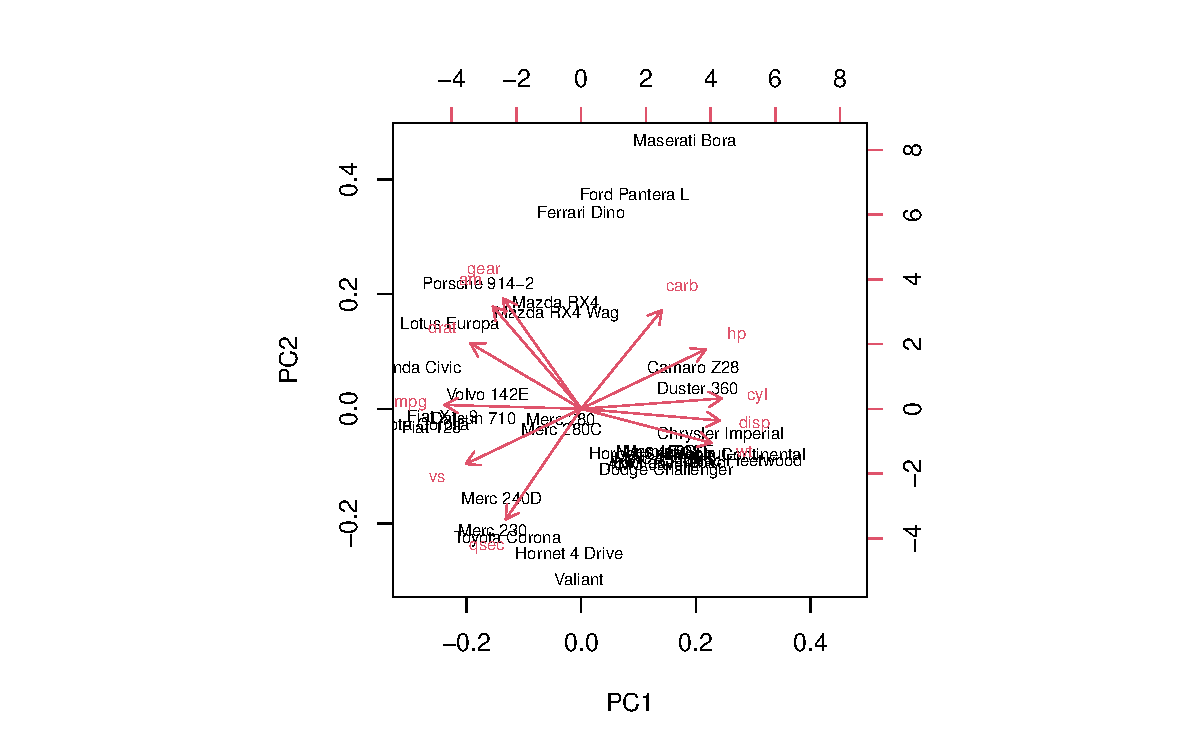
\includegraphics[width=\maxwidth]{figure/beamer-PCAbiplot-1} 

}

\caption[PCA biplots of mtcars dataset]{PCA biplots of mtcars dataset}\label{fig:PCAbiplot}
\end{figure}

\end{knitrout}

\noindent Comparative analysis of these two plots reveals several key findings. The manual construction approach offers meticulous control over the biplot's customisation, allowing for fine-tuning of parameters and appearance. Conversely, the in-built function approach provides a user-friendly ideal for practitioners less inclined towards mathematical intricacies the visualisation. However, despite differences in implementation, both methodologies produce visually comparable biplots, showcasing identical patterns and relationships within the data.

\subsection{Principal Curves}

\noindent Principal curves stand as a vital tool in exploratory data analysis, providing a nonlinear analogue to PCA for capturing the underlying structure of multidimensional data. While PCA focuses on finding linear projections that maximise variance, principal curves seek to identify smooth, nonlinear trajectories that capture the most significant variations in the data. These curves are essentially one-dimensional paths embedded within the multidimensional space of the data points.\\

\noindent Hence, if the points don't fall in a linear subspace, that is, they fall in a non-linear subspace such as a curve in 2-dimension, PCA is insufficient. An example of this is the scatter plot on the left side of Figure~\ref{fig:P-curves}. In this case, a straight line can't be placed in the middle of the plot, however, one could fit a curve that passes through the centre of the points.

\subsubsection{Construction of Principal Curves}

\noindent As with PCA, take $(n \times p)$ data matrix $\mathbf{X}$, with row vectors $\mathbf{x}_i$. The goal is to extract a lower-dimensional set of ``factors" or ``scores" $\mathbf{y} = (y_1, \dots, y_n)^T$. These satisfy the following model:

\[
\mathbf{x}_i = f(y_i) + \epsilon_i, 
\]

\noindent where $\epsilon_i$ are errors with mean 0 and variance $\sigma^2 \mathbf{I}_p$ and $f: \mathbb{R}^1 \rightarrow \mathbb{R}^p$ is a continuous function called a curve \index{Principal curves!curve}\cite{jolliffe2003principal}.\\

\noindent For curve $\mathbf{f}$, the projection index $y_f(\mathbf{x})$ maps observation $\mathbf{x} \in \mathbb{R}^p$ to the point of $\mathbf{f}$ that is closest, returning the score (index). If there are several such points, it returns the largest (this is arbitrary choice to ensure it is a well defined function). Hence, the projection index \index{Principal curves!projection index}is \cite{jolliffe2003principal}: 
\[
y_f(\mathbf{x}) = \sup\limits_{y}\{y: ||\mathbf{x}-\mathbf{f}(y)||= \inf\limits_{\mu}||\mathbf{x}-\mathbf{f}(\mu)||\}.
\]

\noindent As seen in a similar form in PCA, principal curves estimates the following least-squares objective function\index{Principal curves!least-squares objective function}
\[
\min\limits_{\mathbf{f}}\sum_{i=1}^{n} ||\mathbf{x}_i - \mathbf{f}(y_{\mathbf{f}}(\mathbf{x}_i))||^2.
\]

\noindent To construct the principal curve, an algorithm put to work. This iterates between finding a curve $\mathbf{f}$ and then projecting the points onto that. More explicitly, the algorithms \index{Principal curves!algorithm} has the following form \cite{pcurves}: 

\begin{enumerate}
  \item Initialise: let iteration counter $h = 1$ and set $\mathbf{y}^{(0)} = \mathbf{Xu}$, where $\mathbf{u}$ is the first PC vector. 
  \item Smoothing step: With $\mathbf{y}^{(h-1)}$ fixed, estimate $\mathbf{\hat{x}}_i^{(h)}$ with a smoother. 
  \item Projection step: With $\mathbf{\hat{X}}^{(h)}$ fixed, use the projection index to update the scores $\mathbf{y}{(h)}$ so that they have unit speed. 
  \item Loop: Increment $h$ and return to step 1 while the change in the objective function above some threshold.
\end{enumerate}

\subsubsection{Principal Curves in Practice}

\noindent In Figure~\ref{fig:P-curves}, we see an example of how a principal curve is fitted to the observations of an artificial dataset. The points in the plots are not grouped in a linear subspace, but rather follow a similar shape to that of cubic function.\\

\noindent Using the built-in \texttt{principal\_curve()} function, a principal curve can be fitted to the dataset. The principal curve traverses through the densest regions of the data distribution, capturing the underlying nonlinear structure. The panel on the left of Figure~\ref{fig:P-curves} depicts the principal curve overlaid on the dataset, providing insights into the central tendency and inherent curvature of the data. Additionally, whiskers are drawn to visualise the perpendicular distances between data points and the principal curve.

\begin{knitrout}\scriptsize
\definecolor{shadecolor}{rgb}{0.969, 0.969, 0.969}\color{fgcolor}\begin{figure}[H]

{\centering 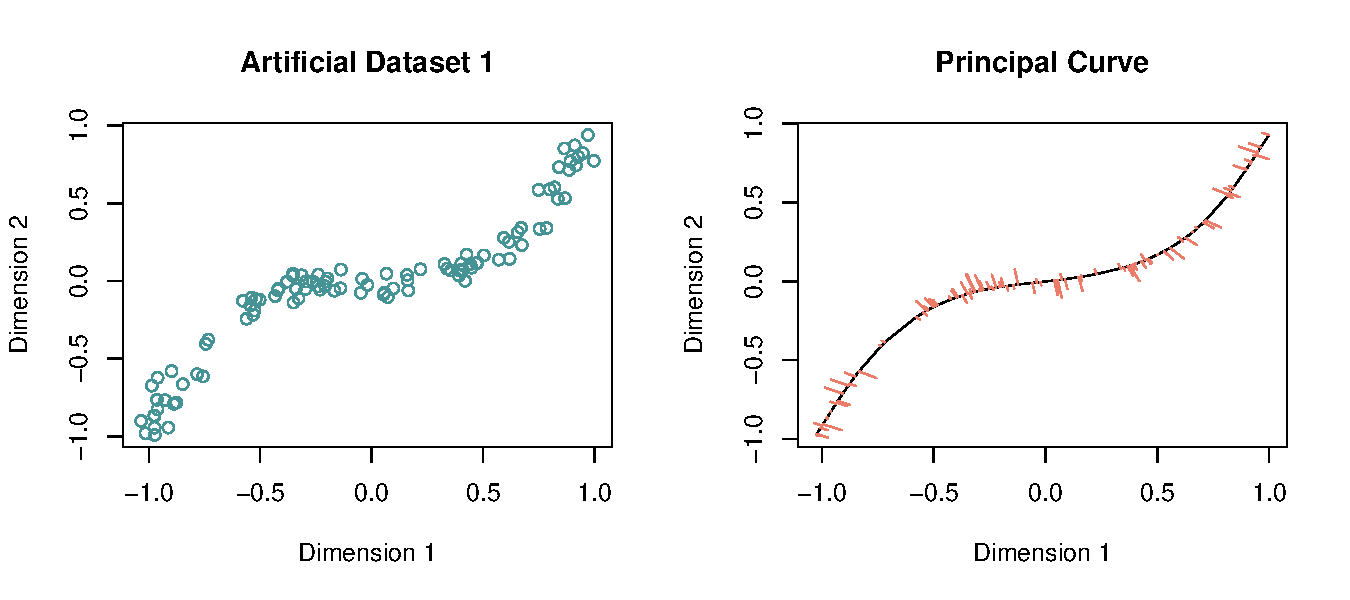
\includegraphics[width=\maxwidth]{figure/beamer-P-curves-1} 

}

\caption[Principal curve fitting illustration on artificial dataset]{Principal curve fitting illustration on artificial dataset}\label{fig:P-curves}
\end{figure}

\end{knitrout}

\noindent The principal curve effectively captures the nonlinear relationship between the dimensions of the artificial dataset. By flexibly adapting to the curvature of the data distribution, the principal curve reveals intricate patterns and trends that may not be captured by linear methods like PCA. The visualisation aids in understanding the underlying structure of the dataset.


\subsection{t-Distributed Stochastic Neighbor Embedding (t-SNE)}

Since PCA is a linear method and may not perform well with non-linear data structures, often missing complex non-linear relationships. Although effective in capturing the global structure of data, PCA focuses on maintaining large pairwise distances to maximise variance and overlooks important local patterns and structures. \\

\noindent
Unlike PCA, t-SNE \cite{vanderMaaten2008tsne} is a nonlinear technique for embedding high-dimensional data for visualisation in a low-dimensional space of two or three dimensions, focusing on preserving the small pairwise similarities between data points thus retain the local structure of the dataset in a lower-dimensional space. It starts by converting high-dimensional Euclidean distances into probabilities that reflect the similarity between points, then maps these points to a lower-dimensional space in a way that tries to preserve these similarities.

\subsubsection{Theory of t-SNE}

For a given high-dimensional dataset $\{x_1,...,x_n\}$, the t-SNE algorithm quantifies the similarity between pairs of data points, $x_i$ and $x_j$, using conditional probabilities \index{t-SNE!conditional probabilities}$p_{j|i}$. These probabilities are calculated under the assumption that if $x_i$ were to choose its neighbours, it would do so in proportion to their probability density under a Gaussian distribution centered at $x_i$. The conditional probability $p_{j|i}$ \cite{vanderMaaten2008tsne} for $i \neq j$ is mathematically expressed as:

\[p_{j|i} = \frac{\exp(-||\mathbf{x}_i - \mathbf{x}_j||^2 / 2\sigma_i^2)}{\sum_{k \neq i}\exp(-||\mathbf{x}_i - \mathbf{x}_k||^2 / 2\sigma_i^2)},\]

\noindent
where $\sigma_i$ denotes the variance of the Gaussian that is centered on data point $x_i$. Also, set similarities of the same pair wise points $p_{i|i}=0$ and $\sum_{j} p_{j|i} = 1$ for all $i$.\\

\noindent
To create a symmetrical joint probability \index{t-SNE!joint probability}distribution in the high-dimensional space, t-SNE averages the conditional probabilities $p_{j|i}$ and $p_{i|j}$ \cite{vanderMaaten2008tsne}, resulting in:
    \[
        p_{ij} = \frac{p_{j|i} + p_{i|j}}{2n},
    \]
    
\noindent
where $n$ is a number of data points. Also, $p_{ii}=0$ and \sum_{i,j} p_{ij}=1$.\\

\noindent
In the low-dimensional space (usually 2D or 3D), we have the corresponding dataset $\{y_1,...,y_n\}$. Since t-SNE aims to find mapped points 
$y_i$ and $y_j$ in a low-dimensional space that reflects the similarities 
$p_{ij}$ as well as possible. In the low-dimensional space, t-SNE computes similarities $q_{ij}$ using a similar formula but with a Student t-distribution (with one degree of freedom, equivalent to the Cauchy distribution) which has heavier tails than a Gaussian distribution to compute the joint probabilities \cite{vanderMaaten2008tsne} of the mapped points:

    \[
        q_{ij} = \frac{(1 + ||\mathbf{y}_i - \mathbf{y}_j||^2)^{-1}}{\sum_{k \neq l}(1 + ||\mathbf{y}_k - \mathbf{y}_l||^2)^{-1}}.
    \]

\noindent
Similarly, set $q_{ii}=0$.\\

\noindent
The goal of t-SNE is to minimize the discrepancy between the probabilities 
$p_ {ij}$ in the high-dimensional space and $q_{ij}$ in the low-dimensional space. Therefore, the objective is to minimise the Kullback-Leibler (KL) divergence \cite{vanderMaaten2008tsne} between the joint probability distributions $P$ and $Q$:
    \[
        C = \text{KL}(P || Q) = \sum_{i \neq j} p_{ij} \log \frac{p_{ij}}{q_{ij}},
    \]
    
\noindent
where the $C$ means the cost function \index{t-SNE!cost function}that we wish to minimize, and the Kullback-Leibler (KL) divergence \index{t-SNE!Kullback-Leibler divergence}is a measure of how probability distribution $P$ differs from probability distribution $Q$. In addition, the lower the KL divergence value, the closer the two distributions are. A KL divergence of zero means that these two distributions are the same.\\

\noindent
To continue with the minimisation, compute the gradient of symmetric SNE \cite{vanderMaaten2008tsne} as follows:
\[\frac{\partial C}{\partial y_i} = 4 \sum_j (p_{ij} - q_{ij})(y_i - y_j)(1 + ||y_i - y_j||^2)^{-1}
.\]

\noindent
Once the gradient of the cost function with respect to the positions of the points in the low-dimensional space, $\frac{\partial C}{\partial y_i}$, is computed, t-SNE employs gradient descent to minimizes the Kullback-Leibler (KL) divergence between the high-dimensional probability distribution $P$ and the low-dimensional probability distribution $Q$. Gradient descent \index{t-SNE!gradient descent}is an iterative optimisation algorithm used to minimize the cost function by updating the parameters in the opposite direction of the gradient of the cost function. In the case of t-SNE, the parameters are the positions of the points in the low-dimensional space. The update rule \cite{vanderMaaten2008tsne} at each iteration $t$ for a point $y_i$ is given by:

\[y_i^{(t+1)} = y_i^{(t)} - \eta \frac{\partial C}{\partial y_i},\]

\noindent
where $\eta$ is the learning rate, a positive scalar determining the step size.\\

\noindent
The process is repeated for a number of iterations or until the change in the cost function between iterations is below a predetermined threshold, indicating convergence. The gradient descent process in t-SNE is crucial for effectively reducing the dimensionality of high-dimensional data while preserving the local structure of the data. By iteratively updating the positions of the points in the low-dimensional space, t-SNE minimizes the KL divergence, resulting in a meaningful representation of the data in lower dimensions.

\subsubsection{Case Example: Classification of Penguins}

In Figure~\ref{fig:t-SNE} we observe a t-SNE visualisation of the penguin dataset. In this case, using the t-SNE algorithm helps us to reduce the multidimensional numerical data of the penguin dataset to a $2$-dimensional space. We also use scatter plots and elliptical areas to visualise the distribution of different penguin species. The data points are colour-coded to distinguish between three penguin species: Adelie in purple, Chinstrap in blue, and Gentoo in red. This colour coding aids in the visual differentiation of the species clusters.\\

\noindent
The axes are labeled $tSNE1$ and $tSNE2$, corresponding to the dimensions reduced by the t-SNE algorithm. Dashed ellipses overlaid on the scatter plot demarcate the clusters of each species, providing a visual guide to the density and separation of the species within the transformed feature space. The plot effectively uses the t-SNE technique to illustrate the grouping of species, highlighting the algorithm's utility in discerning inherent data patterns in a lower-dimensional representation.\\

\begin{knitrout}\scriptsize
\definecolor{shadecolor}{rgb}{0.969, 0.969, 0.969}\color{fgcolor}\begin{kframe}
\begin{alltt}
\hlcom{# PLOT OF T-SNE OF PENGUINS DATASET}
\hlstd{penguins} \hlopt
  \hlkwd{select}\hlstd{(}\hlkwd{where}\hlstd{(is.numeric),}\hlopt{-}\hlstd{year,species)} \hlopt
  \hlkwd{mutate}\hlstd{(}\hlkwc{ID}\hlstd{=}\hlkwd{row_number}\hlstd{())} \hlopt
  \hlkwd{column_to_rownames}\hlstd{(}\hlstr{"ID"}\hlstd{)} \hlopt
  \hlkwd{na.omit}\hlstd{()}\hlkwb{->} \hlstd{df}

\hlstd{tSNE_fit}\hlkwb{<-}\hlstd{df} \hlopt \hlkwd{select}\hlstd{(}\hlopt{-}\hlstd{species)} \hlopt \hlkwd{scale}\hlstd{()} \hlopt \hlkwd{Rtsne}\hlstd{()}
\hlstd{tSNE_fit}\hlopt{$}\hlstd{Y} \hlopt
  \hlkwd{as.data.frame}\hlstd{()} \hlopt
  \hlkwd{rename}\hlstd{(}\hlkwc{tSNE1} \hlstd{=} \hlstr{"V1"}\hlstd{,}\hlkwc{tSNE2} \hlstd{=} \hlstr{"V2"}\hlstd{)} \hlopt
  \hlkwd{mutate}\hlstd{(}\hlkwc{Species} \hlstd{= df}\hlopt{$}\hlstd{species)} \hlkwb{->} \hlstd{tSNE.plot}

\hlcom{# Define custom colors for species}
\hlstd{species_colors} \hlkwb{<-} \hlkwd{c}\hlstd{(}\hlstr{"Adelie"} \hlstd{=} \hlstr{"#4B0082"}\hlstd{,} \hlstr{"Chinstrap"} \hlstd{=} \hlstr{"#459395"}\hlstd{,} \hlstr{"Gentoo"} \hlstd{=} \hlstr{"#EB7C69"}\hlstd{)}

\hlkwd{ggplot}\hlstd{()} \hlopt{+}
  \hlkwd{geom_point}\hlstd{(}\hlkwc{data} \hlstd{= tSNE.plot,} \hlkwd{aes}\hlstd{(}\hlkwc{x} \hlstd{= tSNE1,} \hlkwc{y} \hlstd{= tSNE2,} \hlkwc{color} \hlstd{= Species))} \hlopt{+}
  \hlkwd{stat_ellipse}\hlstd{(}\hlkwc{data} \hlstd{= tSNE.plot,}
               \hlkwc{geom} \hlstd{=} \hlstr{"polygon"}\hlstd{,}
               \hlkwd{aes}\hlstd{(}\hlkwc{x} \hlstd{= tSNE1,} \hlkwc{y} \hlstd{= tSNE2,} \hlkwc{group} \hlstd{= Species,} \hlkwc{fill} \hlstd{= Species),}
               \hlkwc{alpha} \hlstd{=} \hlnum{0.5}\hlstd{,}
               \hlkwc{lty} \hlstd{=} \hlstr{"dashed"}\hlstd{,}
               \hlkwc{color} \hlstd{=} \hlstr{"black"}\hlstd{,}
               \hlkwc{key_glyph} \hlstd{=} \hlstr{"blank"}\hlstd{)} \hlopt{+}
  \hlkwd{scale_color_manual}\hlstd{(}\hlkwc{values} \hlstd{= species_colors)} \hlopt{+}  \hlcom{# Apply custom colors}
  \hlkwd{scale_fill_manual}\hlstd{(}\hlkwc{values} \hlstd{= species_colors)} \hlopt{+}   \hlcom{# Apply custom colors to fill for ellipses}
  \hlkwd{theme_bw}\hlstd{()}
\end{alltt}
\end{kframe}\begin{figure}[H]

{\centering 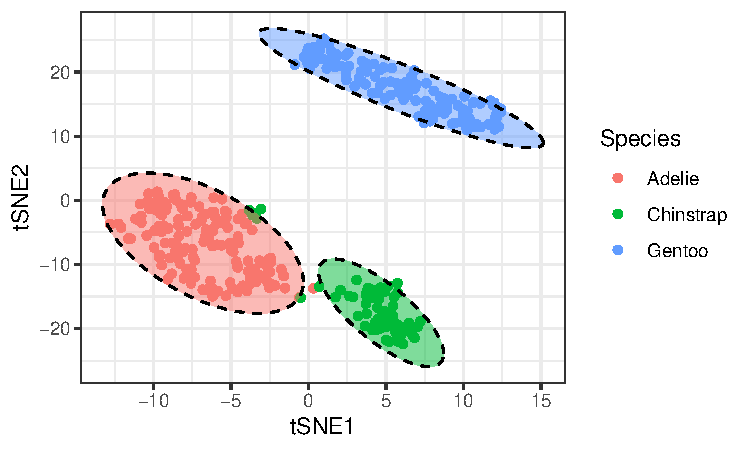
\includegraphics[width=\maxwidth]{figure/beamer-t-SNE-1} 

}

\caption[t-SNE of Penguins Dataset]{t-SNE of Penguins Dataset}\label{fig:t-SNE}
\end{figure}

\end{knitrout}

\noindent
While t-SNE is an exceptionally potent tool for data visualisation, it does come with its own set of constraints. Firstly, it has a significant memory footprint and can be time-consuming to run, which may pose challenges when dealing with large datasets.\\

\noindent
Secondly, t-SNE is tailored specifically for visualisation, which constrains the embedding space to two or three dimensions. This limitation means that t-SNE is optimised for human interpretability rather than for capturing higher-dimensional relationships.\\

\noindent
Additionally, it requires experimentation with different initialisation to mitigate the risk of local sub-optimal solutions affecting the results. Therefore, it's crucial to carefully consider and select the most suitable method based on the specific requirements and nature of the data at hand.

\subsubsection*{Chapter Overview and Further Reading References}

\noindent Chapter 5 explores the theory PCA, and its applications constructing biplots and principal curves, as well as the theory of t-SNE. These concepts date back to 1901 when PCA was first introduced by Karl Pearson \cite{pearson1901liii}. Thus, they are well established in existing literature. Substantial detail on PCA, biplots and principal curves is available in \href{https://link.springer.com/book/10.1007/b98835}{\textit{Principal Component Analysis}} (2003) by Ian T. Jolliffe. Transitioning from PCA, \href{https://www.jmlr.org/papers/volume9/vandermaaten08a/vandermaaten08a.pdf}{\textit{Visualising Data using t-SNE}} (2008) by  Laurens van der Maaten and Geoffrey Hinton is a seminal paper exploring the theory of t-SNE. 

\newpage 

\section{State-Of-The-Art Modern Approaches}

In this chapter, we introduce some state-of-the-art graphical statistical methods published in recent research papers. In Chapter 6.1, we briefly present box plots and Q–Q plots, which set the foundation for the modern visualisation techniques subsequently. Following, the theory and implementation of functional boxplots and Q–Q Box plots is illustrated, as published in recent articles in the \textit{Journal of Computational and Graphical Statistics}. 

\subsection{Introduction}

\subsubsection{Box Plots in Practice}\\

\noindent 
Box plots, also known as box-and-whisker plots, were first introduced by John W. Tukey in 1977 \cite{tukey1977exploratory}. Since then, they have become an extremely popular tool in exploratory data analysis, offering a summary of a dataset's central tendency, skewness, and outliers. These boxplots typically showcase the median, quartiles, and range, making them valuable for comparing and discerning patterns across different variables.\\

\noindent
An example of classic box plots using the iris dataset is displayed on the left of Figure~\ref{fig:box-plots}. Accompanying the box plots, the graph on the right showcases a violin plot — which is a recent advancement in box plot techniques. The violin plot combines a box plot with a kernel density function, providing a mirrored density plot displayed in the same way as a box plot.\\

\begin{knitrout}\scriptsize
\definecolor{shadecolor}{rgb}{0.969, 0.969, 0.969}\color{fgcolor}\begin{figure}[h]

{\centering 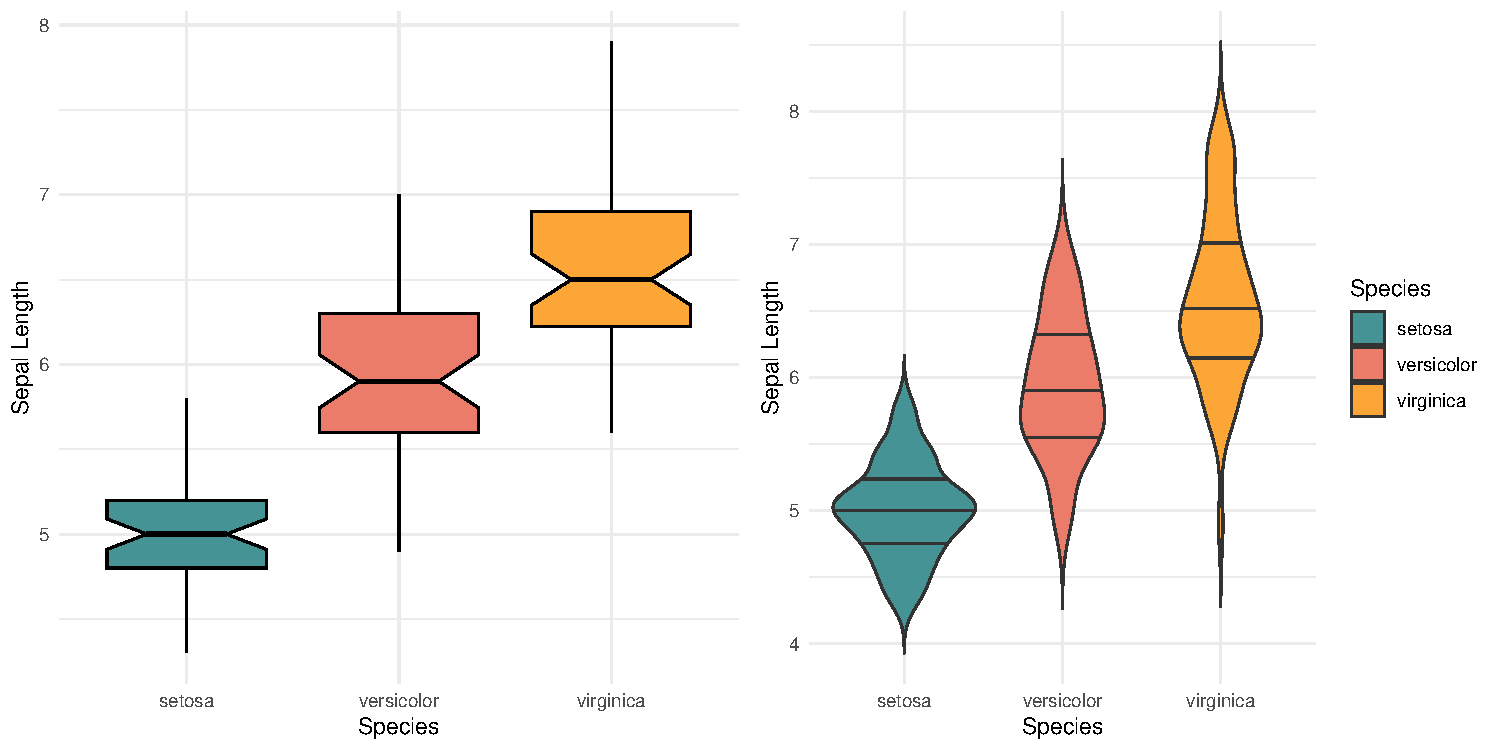
\includegraphics[width=\maxwidth]{figure/beamer-box-plots-1} 

}

\caption[Comparison of Box Plots and Violin Plots of Sepal Length by Species]{Comparison of Box Plots and Violin Plots of Sepal Length by Species}\label{fig:box-plots}
\end{figure}

\end{knitrout}

\subsubsection{Q–Q Plots in Practice}\\

\noindent Q-Q plots, short for quantile-quantile plots, were pioneered by the statistician Francis Galton in the late 19th century \cite{galton1875iv}. These plots are designed to assess the similarity between the empirical distribution of data and a theoretical distribution, often the normal distribution. This comparison provides insights into the degree of similarity between the two, aiding in diagnostics and model validation in statistical analysis.\\

\noindent Q–Q plots are constructed by plotting the quantiles of two datasets against each other. Typically, one dataset serves as the basis for theoretical quantiles, often assumed to follow a particular probability distribution, while the other dataset holds observed values. This comparative depiction allows a direct assessment of how closely the observed data aligns with the theoretical distribution, facilitating the identification of deviations from expected patterns.\\

\noindent In this section, side-by-side Q-Q plots are displayed offering a visual comparison of the distributional properties of two variables from the mtcars and the iris datset. These plots serve as a means to assess normality assumptions and identify potential deviations from expected distributions. Through this visual exploration, we aim to gain insights into the underlying structure of the data and guide further investigation.\\

\begin{knitrout}\scriptsize
\definecolor{shadecolor}{rgb}{0.969, 0.969, 0.969}\color{fgcolor}\begin{figure}[h]

{\centering 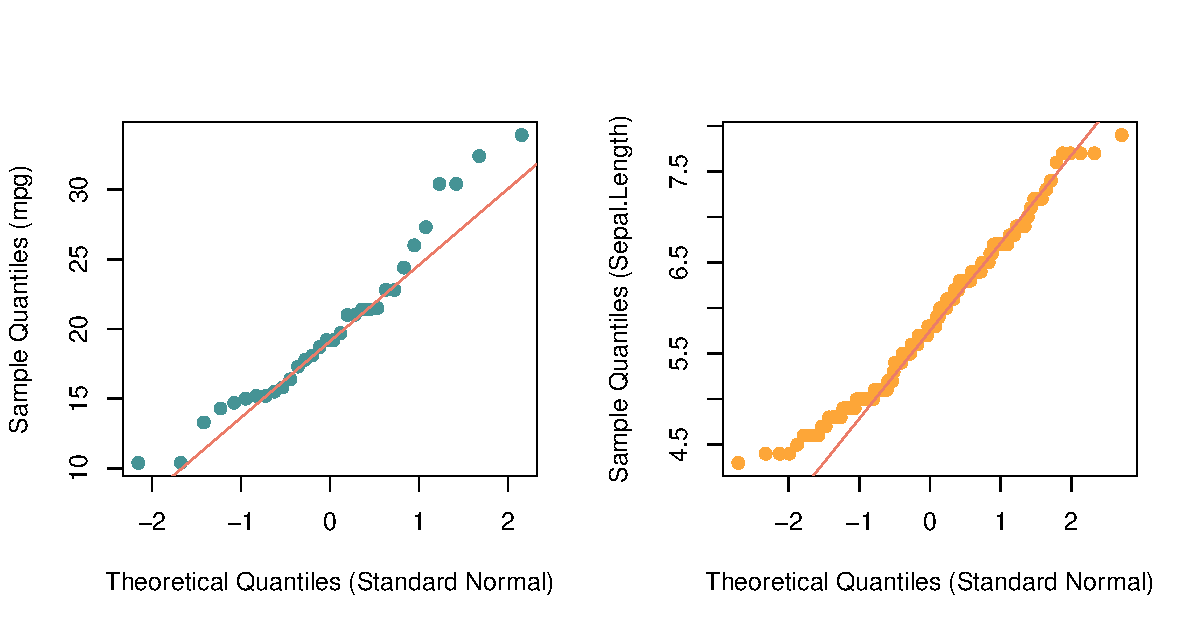
\includegraphics[width=\maxwidth]{figure/beamer-QQplots-1} 

}

\caption[Q–Q plot of mpg in mtcars dataset]{Q–Q plot of mpg in mtcars dataset}\label{fig:QQplots}
\end{figure}

\end{knitrout}

\noindent In the first plot in Figure~\ref{fig:QQplots}, which examines the mpg variable in the mtcars dataset, deviations, particularly in the tails of the distribution, are noticeable. These deviations suggest potential departures from normality, and thus, indicating the presence of outliers or non-normal behaviour in the data.\\

\noindent The second plot examines the distribution of the Sepal.Length variable in the iris dataset. Here, the points exhibit a very slight departure from the theoretical quantiles line. The deviation is far less pronounced compared to the plot on its left. Therefore, indicating that the distribution of sepal lengths within the iris dataset is approximately normal.\\

\noindent In general, the Q–Q plots provide a neat and insightful representation of the distributional properties of the different variables. They provide an effective visual means to assess normality assumptions and to identify potential outliers or deviations from expected distributions, as is the case in the first graph of Figure~\ref{fig:QQplots}. 

\subsection{Functional Boxplot}

\noindent
Building upon the traditional box plot, the functional boxplot is an innovative extension that provides a comprehensive visual representation of functional data. The $i^{th}$ observation of the population is represented as a real function $y_i(t)$, where $i = 1, \dots , n, t \in \mathcal{I}$, where $\mathcal{I}$ is an interval on the real line.\\

\noindent
This section aims to unravel the methodology behind functional boxplots, elucidating their construction, interpretation, and application in real-world datasets, which enables a deeper understanding of the patterns and anomalies inherent in functional data.

\subsubsection{Theory of Funtional Boxplot}

The construction of a box plot relies on data ordering, where you simply arrange univariate observations from smallest to largest. However, with multivariate data, this process becomes significantly more complex, necessitating advanced methodologies to establish a meaningful order. Various versions of data depth have been developed to assess the centrality (or depth) of an observation or its deviation (outlyingness), where observations have a population distribution of density P.\\

\noindent
Consider a set of observations $\{y_1(t),\dots,y_n(t)\}$ defined over an interval $\mathcal{I} \in \mathbb{R}$. The graph of a function $y(t)$ is defined as $G(y) = {(t,y(t)) : t \in I}$. Applying the concept of range from univariate data to two dimensions, we derive a band in $\mathbb{R}^2$ bounded (also known as delimited) by curves $y_{i_1},\dots, y_{i_k}$ for time (or states) $1, \dots, k$. Band \index{Funtional boxplot!band}is defined as $B(y_{i_1},\dots,y_{i_k}) = \{(t,x(t)): t \in \mathcal{I}, \min_{r=1,\dots,k} y_{i_r}(t) \leq x(t) \leq \max_{r=1,\dots,k} y_{i_r}(t)\}$. Let $J$ denote the number of curves that determines the band, where J is a fixed integer $2 \le J \le n$.\\

\noindent
For a stochastic process $Y(t)$ generating the observations $y_1(t), \dots, y_n(t)$, the population version of the band depth \index{Funtional boxplot!band depth}for a curve $y(t)$ with respect to the probability measure P is defined as:

\begin{equation}
BD_{J}(y, P) = \sum_{j=2}^{J} BD^{(j)}(y,P)=\sum_{j=2}^{J} P\{G(y) \subset B(Y_1,\dots,Y_j)\}, 
\end{equation}

\noindent
where $B(Y_1,\dots,Y_j)$ is a band delimited by $j$ random curves \cite{SunGenton2011FunctionalBoxplots}. Here, $BD^{(j)}(y,P)$ calculates the probability that the graph of $y(t)$ lies entirely within a band formed by any selection of $j$ functions. These bands are delineated by the minimum and maximum values at each point $t$ among the selected $j$ functions. This formulation of BD facilitates a nuanced understanding of curve centrality and variability within functional data, laying the groundwork for the construction of functional boxplots. Then we can define the sample version of $BD(j)(y,P)$, which is the fraction of the bands determined by $j$ different sample curves containing the whole graph of the curve $y(t)$ \cite{SunGenton2011FunctionalBoxplots}:

\begin{equation}
BD_{n}^{(j)}(y) = {\binom{n}{j}}^{-1} \sum_{1 \leq i_1 < i_2 < \cdots < i_j \leq n} I\{G(y) \subseteq B(y_{i_1}, \ldots, y_{i_j})\}, 
\end{equation}

\noindent
where $I\{\cdot\}$ denotes the indicator function. Hence, by computing the fraction of the bands containing the curve $y(t)$, the bigger the value of band depth, the more central position the curve has. Then, the sample band depth of a curve $y(t)$ is \cite{SunGenton2011FunctionalBoxplots}

\begin{equation}
BD_{n,J}(y) = \sum_{j=2}^{J} BD^{(j)}_n (y).
\end{equation}

\noindent
A sample median function is a curve from the sample with largest depth value, defined by \cite{SunGenton2011FunctionalBoxplots} 

\begin{equation}
\text{argmax}_{y \in {y_1,\dots,y_n}} BD_{n,J}(y).
\end{equation}

\noindent
In a traditional boxplot, the box represents the central 50\% of the data.  In functional box plot, estimate the central region of data using a band defined by the $\alpha$ proportion (where $0 < \alpha < 1$) of the deepest curves in the sample. Specifically, the central region {Funtional boxplot!central region}for 50\% of the sample, denoted as $C_{0.5}$, is calculated using the formula \cite{SunGenton2011FunctionalBoxplots}:

\begin{equation}
C_{0.5} = \{(t, y(t)) : \min_{r=1, \ldots, \lceil n/2 \rceil} y[r](t) \leq y(t) \leq \max_{r=1, \ldots, \lceil n/2 \rceil} y[r](t)\},
\end{equation}

\noindent
where $\lceil n/2 \rceil$ is the smallest integer not less than half of the sample size. This 50\% central region functions similarly to the inter-quartile range (IQR) in a boxplot, providing a measure of the spread of the central 50\% of the curves. This method is robust, less affected by outliers or extreme values, and offers a clearer visualisation of the distribution's central spread. Within this central region, the curve that represents the median, denoted as $y_{[1]}(t)$, signifies the most centrally located curve with the highest band depth, serving as a robust measure of central tendency.

\subsubsection{Case Example: Visualisation of Metabolic Syndromes}
\noindent
The functional boxplot shown in Figure \ref{fig:fbplot} illustrates the metabolism rates between healthy and diseased populations. The outer blue line highlights a wider range for the diseased group, accompanied by a broader grey band. The range indicates greater variability and the band indicates lower oxygen saturation for most patients in the blood of the diseased group.
\begin{figure}[H]
    \centering
    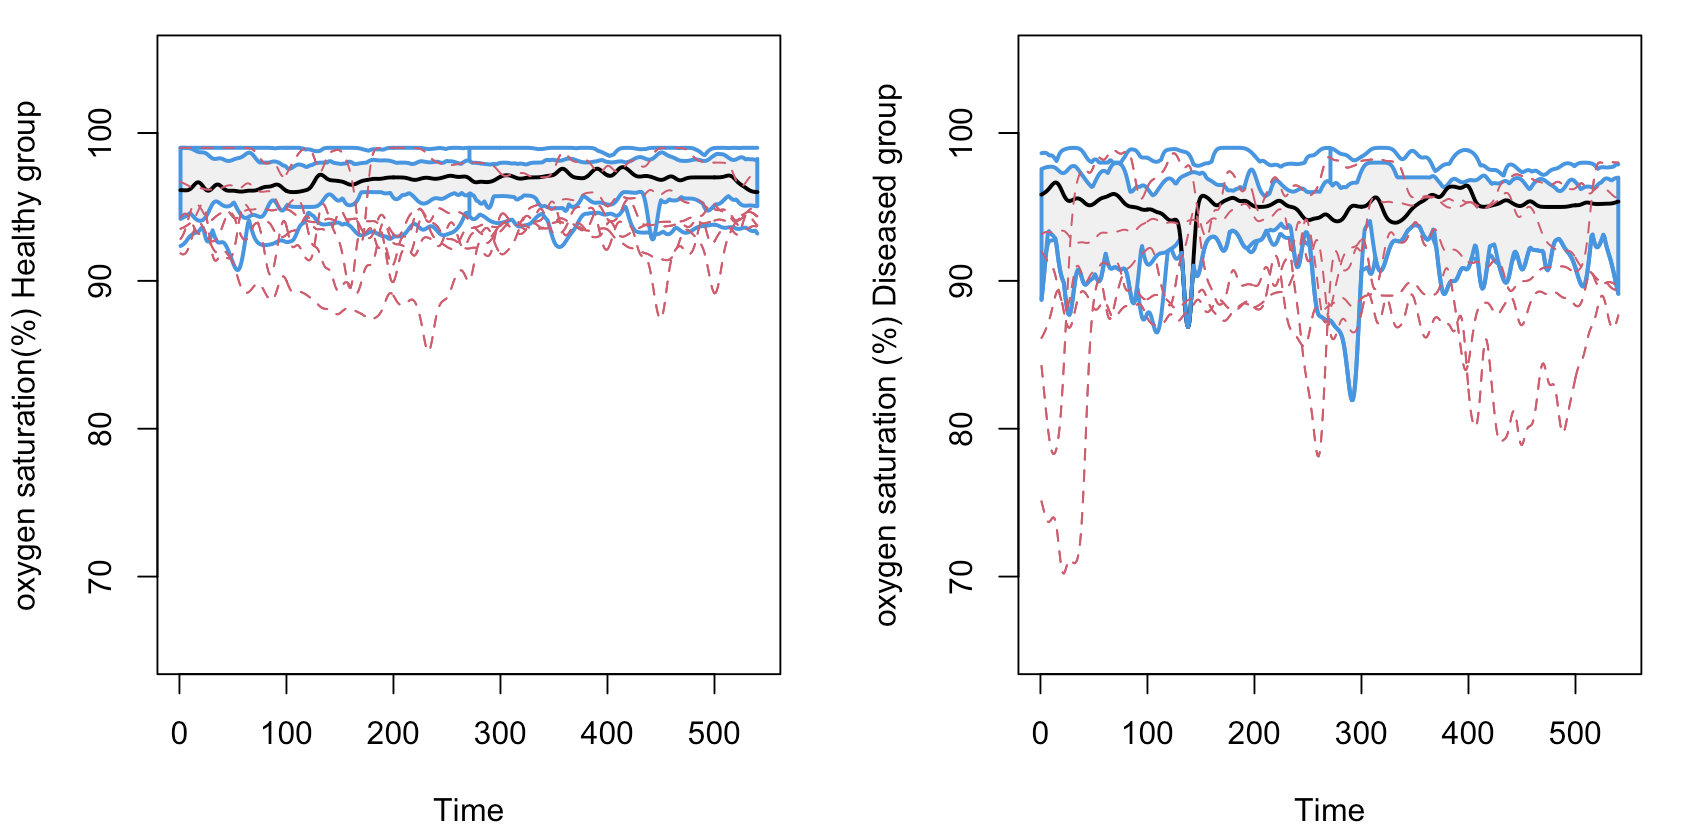
\includegraphics[width=0.8\textwidth]{image_reference/fbplot.png}
    \caption{Arterial Oxygen Saturation (\%) Curves: Women Without vs. With Metabolic Syndrome, Highlighting Outliers}
    \label{fig:fbplot}
\end{figure}

\noindent Left graph in Figure~\ref{fig:fbplot} demostrates curves of arterial oxygen saturation (\%) for 80 women without metabolic syndrome and right graph demostrates curves of arterial oxygen saturation (\%) for 35 women with metabolic syndrome. Outliers from the population are highlighted in red.

\subsection{Q–Q Boxplots}
In this section, we will introduce the Q–Q boxplot, which combines the advantages from the boxplot and the Q–Q plot. The Q–Q boxplot integrates the box plot's ability to summarise data through its quartiles and the Q–Q plot's capability to compare data distributions to a theoretical distribution.\\

\noindent 
Nevertheless, although Q–Q plots and box plots are very effiective in data visualisation, they have certain limitations. Q–Q plots are less effective than box plots in highlighting summary quantitles, and their readability also suffers when multiple samples together are represented together in one plot. Furthermore, box plots usually have unreliable tail information when $n<100$, therefor they may not suitable for research questions that need accurate estimates of extreme quantiles.\\

\subsubsection{Construction of Q–Q Boxplots}
The construction of a Q–Q boxplot involves a three-step process \cite{rodu2022q}. The first setp is to construct the box, similar to that of the standard boxplot, and which represents the interquartile range of the data. The second step is to draw the whiskers and confidence bands. Finally, the third step involves drawing the outside values. The first and third steps of the process mirror exactly those involved in the creation of classic box plots.\\

\noindent
The unique aspect of the Q–Q boxplot comes in the second step. In order to draw the whiskers \index{Quantile–Quantile boxplot!whiskers}and confidence bands, both the comparison distribution and the reference distribution must be standardised. This standardisation process involves matching the quantiles from the reference distribution to those in the comparison distribution, either by subsampling or interpolation. Once this is done, the deviations of the comparison distribution from the reference distribution are calculated relative to each data point\\

\noindent 
Alongside this, the point-wise confidence bands are also determined, which provides a visual indication of how closely the data follows the expected theoretical distribution. To integrate the relative deviations and confidence bands into the Q–Q boxplot, we include both the x and y coordinates in the plot. The y-axis coordinates correspond to the quantile values from the comparison dataset, while the x-axis coordinates represent the deviations relative to the reference distribution.\\

\noindent
To calculate the x-coordinate for a Q–Q boxplot, we set a scale for the plot and determin the maximum x-coordinate, $x_{\text{max}}=(\frac{b_w}{2})$ where $b_w$ is the box width. Let $\text{dev}_{\text{max}$ be the maximum of the absolute values of the whisker deviations and confidence band values. The value of a relative deviaition $d$ is computed by either taking the difference between the standardised values from the comparison distribution and those from the reference distribution, or by using a value from the confidence band associated with the reference distribution. We can then set:
$$x^* = \frac{d \cdot x_{\text{max}}}{\text{dev}_{\text{max}}}.$$
The $x$ coordinate is then $x_b+x*$, where $x_b$ marks the center of the boxplot.

\newpage 

\subsubsection{Case Example: Iris Dataset Using Q–Q Boxplot}

\noindent In R, the \textt{geom\_qqboxplot()} function facilitates the generation of Q-Q boxplots. The resulting Q-Q boxplots produced using this function and the iris dataset are displayed in Figure~\ref{fig:QQboxplots}. These how the distribution of sepal length values within each iris species respectively. The Q-Q boxplots make possible a comparative analysis to assess whether the distributions adhere to a normal distribution assumption. Moreover, as classic boxplots, these Q-Q boxplots also make easy the identification of outliers.\\ 

\begin{knitrout}\scriptsize
\definecolor{shadecolor}{rgb}{0.969, 0.969, 0.969}\color{fgcolor}\begin{figure}[h]

{\centering 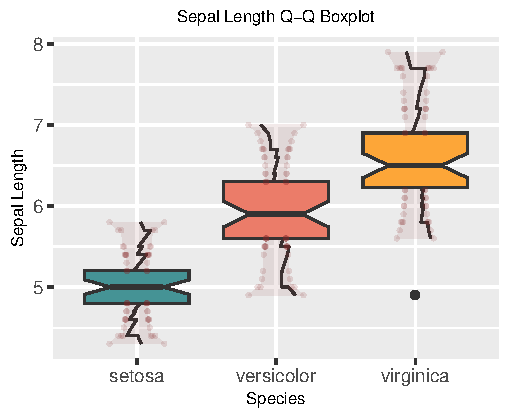
\includegraphics[width=\maxwidth]{figure/beamer-QQboxplots-1} 

}

\caption[Q–Q boxplot of iris dataset]{Q–Q boxplot of iris dataset}\label{fig:QQboxplots}
\end{figure}

\end{knitrout}


\noindent
A brief comparison between Figure~\ref{fig:QQboxplots} and the conventional boxplots depicted in Figure~\ref{fig:box-plots}, shows consistent alignment in the central tendency measures, indicating coherence between the two visualisation techniques.\\

\noindent 
Moreover, the Q-Q boxplot provides more insights into the tail behavior of the distribution, capturing detailed deviations in both right and left tails. Remarkably, all deviations are found the bands of confidence, suggesting a high degree of consistency between the observed sample distribution and the theoretical distribution under scrutiny, notably a normal distribution. 

\subsubsection*{Chapter Overview and Further Reading References}

\noindent This concluding chapter provides an overview of traditional boxplots and Q-Q plots, followed by an examination of modern data visualisation techniques such as functional boxplots and Q-Q boxplots. Despite being relatively new methods, they have garnered attention in the literature. For further understanding of functional boxplots, readers can refer to Ying Sun and Marc G. Genton's article \textit{Functional Boxplots}. Similarly, additional insights into Q-Q boxplots can be found in Jordan Rodu and Karen Kafadar's article \textit{The Q-Q Boxplot}, both of which are published in the \href{https://www.tandfonline.com/journals/ucgs20}{\textit{Journal of Computational and Graphical Statistics}}.

\newpage  


\printindex
  

\newpage

\bibliographystyle{plain} % Choose a style that suits your needs
\bibliography{reference} % The filename of your .bib file

\end{document}
